%Template criado para o PPGCC - UFOP
%Baseado no template da COPPE - UFRJ
%Modificado por Mateus Coelho Silva, M.Sc.

\documentclass[dsc,numbers]{coppe}
%mscexam: qualificação de mestrado
%msc: mestrado
%dscexam: qualificação de doutorado
%dsc: doutorado

\usepackage[utf8]{inputenc}
\usepackage{amsmath,amssymb}
\usepackage{amsthm}
\usepackage{epigraph}
\usepackage{stfloats}
\usepackage{hyperref}
\usepackage[intoc]{nomencl}
\usepackage{etoolbox}
\usepackage{subcaption}
\usepackage[final]{pdfpages}
\usepackage{listings}
\usepackage{multirow}
\usepackage{graphicx}
\usepackage{booktabs}

\captionsetup{compatibility=false}
\theoremstyle{definition}
\newtheorem{definition}{Definition}
\setlength\epigraphwidth{.8\textwidth}
\setlength\epigraphrule{0pt}


\makelosymbols
\makeloabbreviations
\makenomenclature

\begin{document}
  \title{Wearable Edge AI towards Cyber-Physical Applications}
  \foreigntitle{Wearable Edge AI towards Cyber-Physical Applications}
  \author{Mateus Coelho}{Silva}
  \advisor{Prof.}{Ricardo Augusto Rabelo}{Oliveira}{Dr.}
  \advisor{Prof.}{Servio Pontes}{Ribeiro}{Dr.}
  \advisor{Prof.}{Andrea Gomes Campos}{Bianchi}{Dr.}

%   \examiner{Prof.}{Ricardo Augusto Rabelo Oliveira}{Dr.}
%   \examiner{Prof.}{Servio Pontes Ribeiro}{Dr.}
%   \examiner{Prof.}{Andrea Gomes Campos}{Bianchi}{Dr.}
  %\examiner{Prof.}{Saul Emanuel Delabrida Silva}{Dr.}
  %\examiner{Prof.}{José Augusto Miranda Nacif}{Dr.}
  \department{DECOM}

  \keyword{Edge AI}
  \keyword{Cyber-Physical Systems}
  \keyword{Wearable Computing}
  \keyword{Computer Vision}
  \maketitle
  %\includepdf{ficha.pdf}
  %\includepdf{ata.pdf}
  
  \dedication{ ``The day we cease the exploration of the cosmos is the day we threaten the continuing of our species. In that bleak world, arms-bearing, resource-hungry people \& nations would be prone to act on their low-contracted prejudices and would have seen the last gasp of human enlightenment... until the rise of a visionary new culture that once again embraces the cosmic perspective. A perspective in which we are one, fitting neither above nor below, but within.'' \\ {Neil DeGrasse Tyson}}
%\newpage\null\thispagestyle{empty}\newpage
  \include{thanks}
  \include{resumo}
  \begin{foreignabstract}

The creation of novel technologies to support field work and research has a major impact from technologies such as the Internet of Things (IoT), Edge Computing and wearable computing. In this context, Artificial-Intelligence-based systems became more common and a trend in recent work. Environments with low connectivity and high latency in data transmission enforce the usage of Edge Computing technologies in the treatment of acquired data. Nonetheless, there is no clarity in how to transport Artificial Intelligence (AI) to Edge Computing in extreme environments, given the complexity of the requirements. This gap is more clear in the context of wearable computing, where the systems restrictions for developing systems are even harder. Thus, this work presents a protocol for developing Edge AI appliances and some case-study applications in the context of wearable devices. This study helps to evaluate the creation of Wearable Edge AI context as a novel research field.

\end{foreignabstract}
  \renewcommand{\nomname}{List of Abbreviations}
  %Nova abreviação: \nomenclature{HW}{Hardware} 
  \selectlanguage{english}
  \tableofcontents
  \listoffigures
  \listoftables
  \printlosymbols
  \printnomenclature

  \mainmatter
  \chapter{Introduction}
\label{chap:intro}

\nomenclature{CPS}{Cyber-Physical System}
\nomenclature{IoT}{Internet of Things}
\nomenclature{ZB}{Zettabytes}
\nomenclature{NLP}{Natural-Language Processing}

Cyber-Physical Systems (CPSs) are a nomenclature created to describe the applications that combine digital aspects with real-world applications. This integration happens through an integrated loop using sensors to add perception and often actuators to interact with the environment \cite{zanero2017cyber}. Some of the essential aspects that enable the development of such systems are hardware miniaturization and the increased number of devices with networking abilities \cite{alguliyev2018cyber}.

Cyber-physical systems relate to some aspects of computer science, especially within the context of embedded computing and edge computing. Among these aspects, we highlight the following related context \cite{alguliyev2018cyber, baheti2011cyber}:

\begin{itemize}
    \item Industry 4.0;
    \item Internet of Things (IoT);
    \item Big data;
    \item Cloud computing;
    \item Edge computing;
    \item Wearable devices;
    \item Mobile devices;
    \item Real-time systems;
\end{itemize}

Our understanding is that these concepts are linked through two fundamental features of cyber-physical systems. The first important concept we raise is the \textbf{context awareness}. Applications of CPSs must have means to perceive the context around them. Then, the second context is \textbf{environmental interaction}. These applications must be able to interact with the users, stakeholders, and the surrounding environment. Besides these main concepts, some of the features from CPSs are \cite{shi2011survey}:

\begin{itemize}
    \item Closely integrated systems;
    \item Resource constrained;
    \item Networked;
    \item Executes in closed loops;
    \item Reliable and secure.
\end{itemize}

Modeling CPSs is a challenge \cite{derler2011modeling}. Applications within this range must integrate system specifications, considering physical restraints, hardware and software integration, and the network interconnecting the devices. Also, software development in CPSs must consider its correctness and often timing constraints.

In this text, we will henceforth name the applications built within the CPS range as cyber-physical applications. Some examples of stakeholders from cyber-physical applications are smart cities, industries, aviation, environmental monitoring agencies and researchers, healthcare professionals and patients, and meteorologists \cite{alguliyev2018cyber, baheti2011cyber, zanero2017cyber, haque2014review}.

As stated before, wearable computing and edge computing are essential concepts within the range of CPSs. In this work, we explore how to use both these concepts together with artificial intelligence algorithms to create cyber-physical applications. In the following sections, we offer an initial individual perspective on each of these concepts before presenting the main objective of this thesis.

\section{Wearable Computing}

A relevant topic among CPSs is wearable computing, which creates several cyber-physical applications. Steve Mann and Thad Starner took some pioneer steps towards wearable computing in the late 80s and early 90s \cite{mann1997wearable, starner1996human}. Mann \cite{mann1997wearable} enforced that a critical component in the creation of these systems was hardware miniaturization. Starner \cite{starner1996human} had an early understanding of the issues of creating these applications, enforcing the difficulty in energy availability, weight, and size.

Since then, wearable computing has reached various stakeholders with various applications. Roggen et al. \cite{roggen2011wearable} pointed out several uses of wearable computing in robotics and automation, even with gesture and activity recognition. Jhajharia et al. \cite{jhajharia2014wearable} enforce the usage of such systems in healthcare and medical appliances, fitness, wellness, military, and industry.

Wearable computing shares some standard features among their applications \cite{jhajharia2014wearable}. Some of the main features of these systems are:

\begin{itemize}
    \item \textbf{Reliabiliy:} Wearable computers and systems must be consistent and reliable;
    \item \textbf{Context awareness:} Wearable computing systems must add or enhance the user's environmental perception;
    \item \textbf{Ease of use:} Wearable systems must be easy to use, often not requiring any interaction to perform their duties;
    \item \textbf{Non-obstrusive and mobile:} Wearable systems must preserve the users' ability to move freely. 
\end{itemize}

From this perspective, we notice that several of these features come from the broader field of CPSs. Therefore, within our context, we consider wearable computing systems to be examples of cyber-physical applications. 

Wearable devices are trending topics in different areas such as healthcare and activity recognition~ \cite{soh2015wearable,risling2017educating,vogenberg2018healthcare, liu2015sensor, zhang2018pea, qiu2018body, pace2018edge}, sports \cite{kaya2019wearable,camomilla2018trends}, education \cite{fu2018trends,chang2018trends}, industry \cite{kong2018industrial,rice2018evaluating}, human--computer interaction \cite{li2018hand} and other areas. The rise of new concepts like the Internet of Things (IoT) \cite{haghi2017wearable,bhatt2017internet,constant2017fog} and Industry 4.0 \cite{kong2018impact} along with hardware miniaturization allow for the development of novel devices and solutions. Furthermore, the communication aspect of wearable systems is an essential aspect of novel developed solutions \cite{kos2019challenges,li2017smartphone}.

\section{Edge Computing}

The following fundamental concept within this work is Edge Computing. This expression refers to using tools closer to the user's end and further away from the cloud. According to Varghese et al. \cite{varghese2016challenges}, the motivations for this movement include decentralized computing, low latency, sustainable energy consumption, and smart computation techniques. These authors exemplify that the distance between Berkeley and Canberra causes a latency of 175 ms, which imposes an issue for latency-sensitive algorithms. Furthermore, the added network traffic can cause uncertainty.

Cao et al. \cite{cao2020overview} enforce that the expected global traffic on the internet in 2019 was 10.4 Zettabytes (ZB). They assert that 45\% of this information would be stored, processed, and analyzed on the network's edge. By 2020, the number of connected devices was expected to surpass 50 billion. These authors also realized that cloud computing came short on some restraints, namely:

\begin{itemize}
    \item Real-time;
    \item Energy consumption;
    \item Security;
    \item Privacy;
\end{itemize}

Both authors agree on the understanding that there are some issues that are not solved within the domain of cloud computing. Even with the 5G networks, these issues still need to be solved. El-Shorbagy \cite{el20215g} enforces that although 5G networks are faster and have low latencies in the ideal functioning scenario, there are issues as any physical obstacle blocks its signal and it has a lower range.

Khan et al. \cite{khan2019edge} also enforce that fast computing and quick application response are some of the features expected from edge computing, making it more suitable for real-time applications. He presents a division of edge computing among three main areas: \textit{cloudlets}, \textit{fog computing}, and \textit{mobile edge computing}. 

\textit{Cloudlets} are infrastructures with high processing power that perform the role of cloud computing closer to the end-users. \textit{Fog computing} is the virtualization of cloud-like services using a distributed computing environment through mobile devices. \textit{Mobile edge computing} is the processing through isolated or restricted edge computing platforms providing processing power at the very edge of the network.

Khan et al. \cite{khan2019edge} also affirm that edge computing can have a dense geographical distribution, supports mobility, is closer to the end-user, enforces low latency solutions, and provides context-awareness. Finally, the authors display heterogeneity as an aspect of edge computing, given the diversity of devices involved in communication and processing.

Current technologies and environmental conditions still require storage, processing, and analyses at the network's edge. Edge computing is relevant in several cyber-physical applications, including cooperative wearable systems. In this study, this concept has a critical role in creating novel applications using wearable computing and AI techniques.

\section{Artificial Intelligence (AI)}

By the time this work was published, Artificial Intelligence had been a topic of research and development by scientists and engineers for almost 70 years. Jiang et al. \cite{jiang2022quo} presented some projections for the near future of AI, stating that its market share is projected to reach over 190 billion US dollars by 2025. They exemplify some fields of acting from AI, such as:

\begin{itemize}
	\item Speech recognition;
	\item Image processing;
	\item Natural-language processing (NLP);
	\item Smart robots;
	\item Autonomous vehicles;
	\item Healthcare;
\end{itemize}

Besides these, there are numerous fields in which AI has been applied. Jiang et al. \cite{jiang2022quo} also assess some of the facts that enabled the uprise of AI. According to them, the increased number of theoretical proposals, the increasing amount of available data, the increasing computing power, and the outperformance of humans in some tasks of interest have contributed to an increasing interest over the years, starting from the 80s.

In a Q\&A paper published in 2007, McCarthy \cite{mccarthy2007artificial} offers a simple definition of Artificial Intelligence. He states that AI is the science and engineering of making intelligent machines, especially intelligent software. This definition is a simple approach but requires a definition of intelligence. Still, according to McCarthy \cite{mccarthy2007artificial}, intelligence is the ability to achieve goals in the world.

Shinde and Shah \cite{shinde2018review} present machine learning in computer science as the process of creating so-called ``intelligent agents''. In their perception, these agents are capable of perceiving the environment and acting to maximize its opportunity for success. Although artificial intelligence concepts came from the 1950s, the hardware and software advances allowed it to reach the desired potential later on. From the general concept of AI, these advances led to the uprise of machine learning and deep learning. Figure \ref{fig:ml-hierarchy} displays the hierarchy of these concepts according to Shinde and Shah.

\begin{figure}[h!]
    \centering
    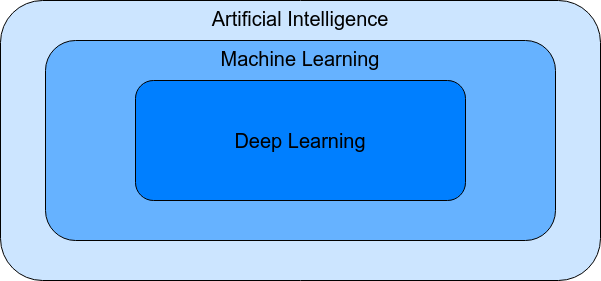
\includegraphics[width=.7\linewidth]{Figures/AI-ML-DL.png}
    \caption{Machine Learning Hierarchy (inspired from Shinde and Shah \cite{shinde2018review})}
    \label{fig:ml-hierarchy}
\end{figure}

Most AI applications follow the process described in the previous paragraph. The set of algorithms that follow this is called machine learning (ML) \cite{el2015machine}. More recently, the most extensive set of algorithms developed is called deep learning (DL) \cite{lecun2015deep,gunning2019xai}, a subset of machine learning algorithms with multiple processing layers to learn abstract data representations.

However, machine and deep learning often find limitations when integrating with edge computing. This condition happens especially when the computing power of the edge application is constrained. Liu et al. \cite{liu2020survey} assert that although many research projects try to reduce this gap, machine, and deep learning often require high computational power and energy consumption. Sze et al. \cite{sze2017hardware} also state that these applications require significant computational power, pushing applications toward the clouds.

\section{Stakeholders}

There are two main stakeholders to the technologies developed in this context. The first stakeholders are professors, students, practitioners, and ecology researchers. The technologies within this context were created aiming for canopy studies and entomology needs. These appliances are usually driven towards environmental perception. Figure \ref{fig:stakeholder-eco} displays some applications developed for these stakeholders.

\begin{figure}[h!]
    \centering
    \includegraphics[width = \linewidth]{Figures/stakeholder-eco.png}
    \caption{Examples of applications developed towards the first stakeholders. These solutions include automatic ant-counting using CNNs, leaf disease detection, and leaf shape estimation.}
    \label{fig:stakeholder-eco}
\end{figure}

The second stakeholders are researchers, physiologists, medical practitioners, patients, and people who require health monitoring appliances. These technologies aim to monitor the users' health conditions and their activities. These applications usually focus on perceiving the users' activities and conditions. Figure \ref{fig:stakeholder-health} displays some applications developed for the second group of stakeholders.

\begin{figure}[h!]
    \centering
    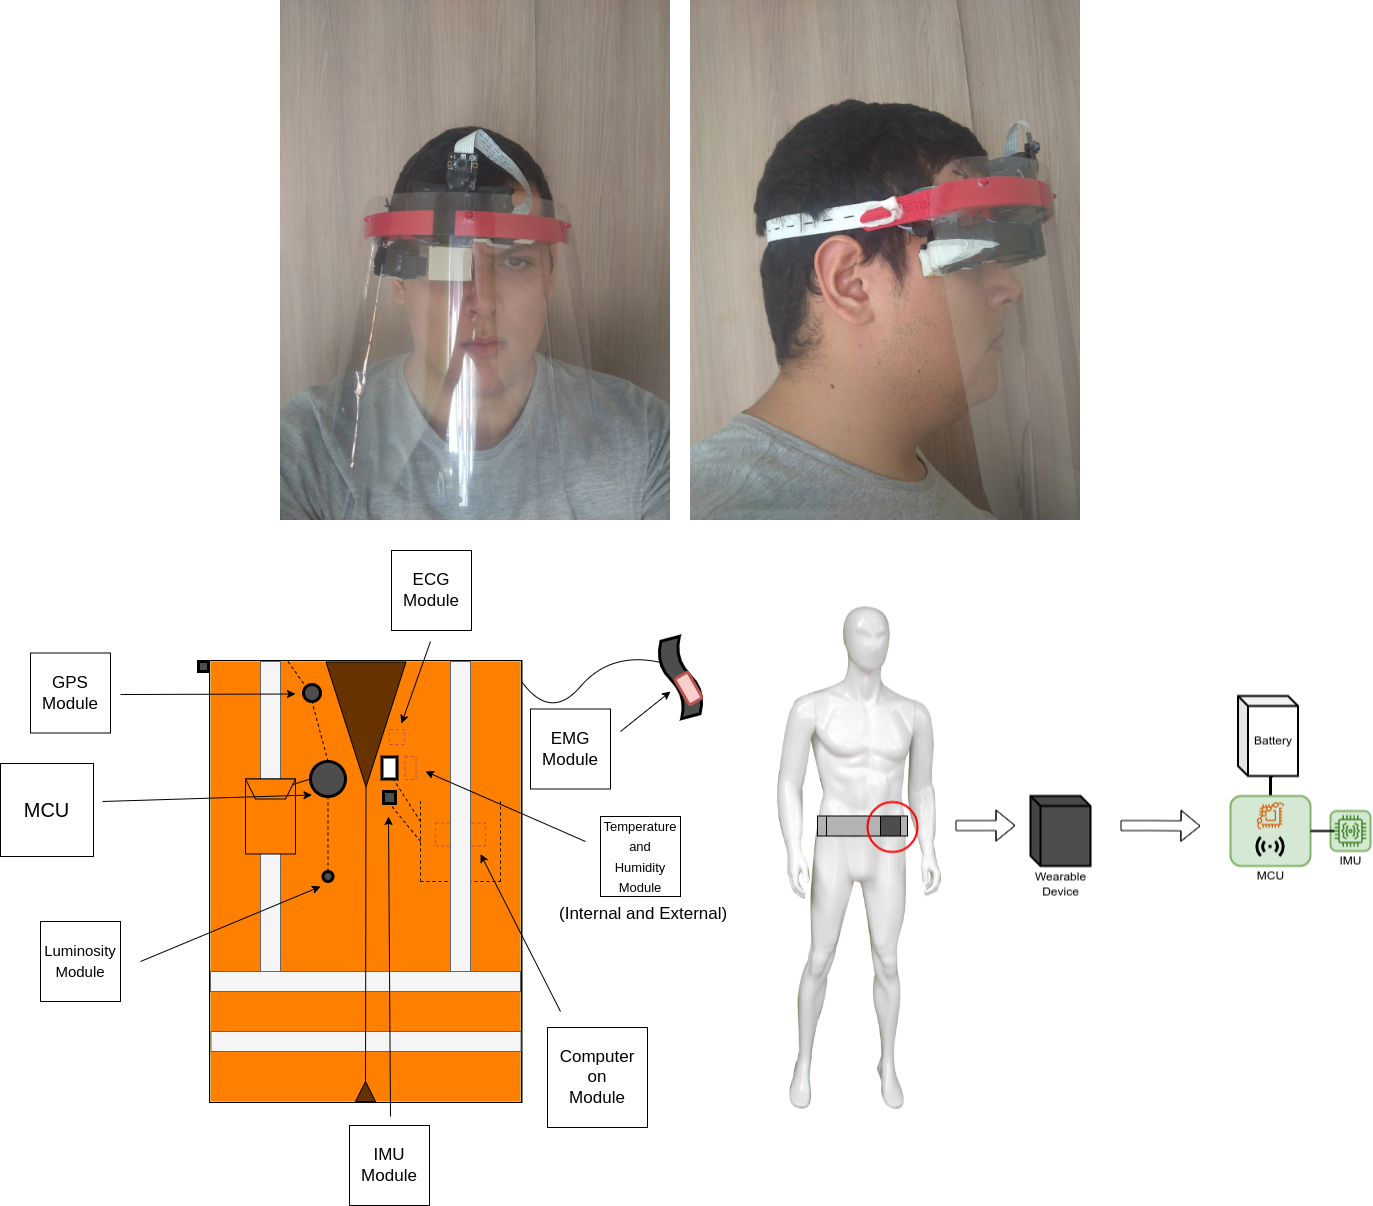
\includegraphics[width = \linewidth]{Figures/stakeholder-health.png}
    \caption{Examples of applications developed towards the second stakeholders. These solutions include health monitoring using a faceshield, a multi-sensored smart vest for industrial applications, and a human activity recognition (HAR) monitor.}
    \label{fig:stakeholder-health}
\end{figure}

\section{Objectives}

In this work, we focus on understanding how to mesh the concepts of edge computing, wearable computing, and AI to create a novel concept within Cyber-Physical Systems. A relatively novel concept named Edge AI works as a baseline for starting this establishment. Therefore, the main objective of this work is:

\begin{itemize}
    \item Establish the concept of Wearable Edge AI and its design process to create cyber-physical applications.
\end{itemize}

We also contemplate a set of specific objectives withing this context. They are:

\begin{itemize}
    \item Propose a novel taxonomy to describe the modalities of Edge AI; 
    \item Develop a set of cyber-physical applications aiming ecological studies;
    \item Develop a set of cyber-physical applications aiming healthcare and human-activity recognition; 
\end{itemize}

\section{Text Organization}

This text is organized into six chapters. In this first chapter, we introduce the subject of the study, motivation, stakeholders, objectives, and contributions. Chapter \ref{chap:establishing} reviews the Edge AI concept and establishes a taxonomy to describe it. Chapter \ref{chap:wearable-edge-ai} displays how we evolved the concept of Wearable Edge AI and defined its design patterns. Chapter \ref{chap:ecology} discusses the applications developed aiming at the ecology stakeholders. Chapter \ref{chap:healthcare} discusses the applications developed aiming at healthcare stakeholders. Finally, we discuss the learned lessons, conclusions, and final remarks in Chapter \ref{chap:conclusions}. 

\section{Contributions}

Within this work's context, we have published the following articles, with a total of 28 citations according to the Google Scholar metrics:

\begin{itemize}
    \item An Automatic Ant Counting and Distribution Estimation System Using Convolutional Neural Networks \cite{Silva2023iceis};
    \item Designing a Multiple-User Wearable Edge AI system towards Human Activity Recognition (2022 XII Brazilian Symposium on Computing Systems Engineering (SBESC)) \cite{silva2022designing};
    \item Edge Computing Smart Healthcare Cooperative Architecture for COVID-19 Medical Facilities (IEEE Latin America Transactions 2022) \cite{silva2022edge};
    \begin{itemize}
        \item 1 citation (Google Scholar);
    \end{itemize}
    \item Bringing Deep Learning to the Fields and Forests: Leaf Reconstruction and Shape Estimation (SN Computer Science, 2022) \cite{silva2022bringing}; 
    \item Wearable Edge AI applications for Ecological Environments (Sensors, 2021) \cite{silva2021wearable};
    \begin{itemize}
        \item 7 citations (Google Scholar);
    \end{itemize}
    \item An Improved Deep Learning Application for Leaf Shape Reconstruction and Damage Estimation (Proceedings of the 23rd International Conference on Enterprise Information Systems - Volume 1: ICEIS, 2021) \cite{iceis21leaf}
    \begin{itemize}
        \item 4 citations (Google Scholar);
        \item Best Student Paper Award in the Area of Artificial Intelligence and Decision Support Systems;
    \end{itemize}
    \item Faceshield HUD: Extended Usage of Wearable Computing on the COVID-19 Frontline (Proceedings of the 23rd International Conference on Enterprise Information Systems - Volume 1: ICEIS, 2021) \cite{iceis21faceshield};
    \begin{itemize}
        \item 1 citation (Google Scholar);
    \end{itemize}
    \item IDiSSC: Edge-computing-based Intelligent Diagnosis Support System for Citrus Inspection (Proceedings of the 23rd International Conference on Enterprise Information Systems - Volume 1: ICEIS, 2021) \cite{iceis21orange};
    \begin{itemize}
        \item 4 citations (Google Scholar);
    \end{itemize}
    \item Leaf shape reconstruction and damage estimation using a U-net-based conditional GAN (Proceedings of the 36th Annual ACM Symposium on Applied Computing - SAC'21, 2021) \cite{silva2021leaf};
    \item Constraints and Challenges in Designing Applications for Industry 4.0: A Functional Approach (Proceedings of the 22nd International Conference on Enterprise Information Systems - Volume 1: ICEIS, 2020) \cite{iceis20robotics};
    \begin{itemize}
        \item 1 citation (Google Scholar);
    \end{itemize}
    \item Field Research Cooperative Wearable Systems: Challenges in Requirements, Design and Validation (Sensors, 2019) \cite{silva2019field};
    \begin{itemize}
        \item 10 citations (Google Scholar);
    \end{itemize}
\end{itemize}

In this period, I have also collaborated with these works with relevant contributions to this topic's knowledge, with 20 more citations:

\begin{itemize}
    \item Towards a mobile system with a new wearable device and an AI application for walking and running activities (Anais do L Semin{\'a}rio Integrado de Software e Hardware, 2023) \cite{alvim2023towards};
    \item A Mobile Robot Based on Edge AI (Anais do L Semin{\'a}rio Integrado de Software e Hardware, 2023) \cite{santos2023mobile};
    \item Towards Autonomous Mobile Inspection Robots Using Edge {AI} (Proceedings of the 25th International Conference on Enterprise Information Systems - Volume 1: ICEIS, 2023) \cite{Santos2023};
    \item Towards a Novel Edge AI System for Particle Size Detection in Mineral Processing Plants (Proceedings of the 25th International Conference on Enterprise Information Systems - Volume 1: ICEIS, 2023) \cite{Cardoso2023};
    \item Blockchain-Based Smart Contract and Edge AI Applied in a Multirobot System: An Approach (IEEE Robotics and Automation Magazine, 2023) \cite{garrocho2023blockchain};
    \item Using Mobile Edge AI to Detect and Map Diseases in Citrus Orchards (Sensors, 2023) \cite{da2023using};
    \begin{itemize}
        \item 2 citations (Google Scholar);
    \end{itemize}
    \item Towards novel smart wearable sensors to classify subject-specific human walking activities (Anais Estendidos do XII Simp{\'o}sio Brasileiro de Engenharia de Sistemas Computacionais) \cite{da2022towards2};
    \item A novel intelligent mobile application using human-centered AR: A case study in orange inspection (Anais Estendidos do XXI Simp{\'o}sio Brasileiro de Fatores Humanos em Sistemas Computacionais) \cite{da2022novel};
    \begin{itemize}
        \item 1 citation (Google Scholar);
    \end{itemize}
    \item Enabling Digital Twins in Industry 4.0 \cite{vitor2022enabling};
    \begin{itemize}
        \item 3 citations (Google Scholar);
    \end{itemize}
    \item Edge Deep Learning Towards the Metallurgical Industry: Improving the Hybrid Pelletized Sinter (HPS) Process \cite{de2022edge};
    \begin{itemize}
        \item 1 citation (Google Scholar);
    \end{itemize}
    \item Towards a novel wearable solution for citrus inspection using Edge AI (2022 IEEE 46th Annual Computers, Software, and Applications Conference (COMPSAC)) \cite{da2022towards};
    \begin{itemize}
        \item 1 citation (Google Scholar);
    \end{itemize}
    \item Applying Edge AI towards Deep-learning-based Monocular Visual Odometry Model for Mobile Robotics (Proceedings of the 24th International Conference on Enterprise Information Systems - Volume 1: ICEIS, 2022) \cite{de2022applying};
    \begin{itemize}
        \item 2 citations (Google Scholar);
    \end{itemize}
    \item Mask R-CNN Applied to Quasi-particle Segmentation from the Hybrid Pelletized Sinter (HPS) Process (Proceedings of the 17th International Joint Conference on Computer Vision, Imaging and Computer Graphics Theory and Applications (VISIGRAPP 2022) - Volume 4: VISAPP) \cite{visapp22hps};
    \item Deep Learning Approach at the Edge to Detect Iron Ore Type (Sensors, 2022) \cite{klippel2022deep};
    \begin{itemize}
        \item 1 citation (Google Scholar);
    \end{itemize}
    \item Deep-Learning-Based Embedded ADAS System (Proceedings of the XI Brazilian Symposium on Computing Systems Engineering (SBESC)) \cite{de2021deep};
    \item Deep-Learning-Based Visual Odometry Models for Mobile Robotics (Proceedings of the XI Brazilian Symposium on Computing Systems Engineering (SBESC)) \cite{de2021deep2};
    \begin{itemize}
        \item 2 citations (Google Scholar);
    \end{itemize}
    \item Synchronous and Asynchronous Requirements for Digital Twins Applications in Industry 4.0 (Proceedings of the 23rd International Conference on Enterprise Information Systems - Volume 1: ICEIS, 2021) \cite{iceis21dt};
    \begin{itemize}
        \item 4 citations (Google Scholar);
    \end{itemize}
    \item Edge Deep Learning Applied to Granulometric Analysis on Quasi-particles from the Hybrid Pelletized Sinter (HPS) Process (Proceedings of the 23rd International Conference on Enterprise Information Systems - Volume 1: ICEIS, 2021) \cite{iceis21hps};
    \begin{itemize}
        \item 3 citations (Google Scholar);
    \end{itemize}
\end{itemize}

We have also deposited a patent request, with its text already in public domain:

\begin{itemize}
    \item ESCUDO FACIAL PARA PROTEÇÃO CONTRA O COVID-19 E DOENÇAS INFECCIOSAS COM MONITOR PORTÁTIL PARA MONITORAMENTO DA SAÚDE DO USUÁRIO E VARIÁVEIS DO AMBIENTE. 2022, Brazil. Registration number: BR1020220014477, INPI - Instituto Nacional da Propriedade Industrial, Brazil.
\end{itemize}

Our total contributions add up to 29 research papers and a deposited patent request, with 48 citations up to this date. We also have two more papers invited to become book chapters. 


\cleardoublepage
  \chapter{Edge AI}
\label{chap:establishing}

\nomenclature{AI}{Artificial Intelligence}
\nomenclature{UAV}{Unmanned Aerial Vehicles}
\nomenclature{WSN}{Wireless Sensor Networks}
\nomenclature{HPS}{Hybrid Pelletized Sinter}
\nomenclature{VANET}{Vehicular Ad Hoc Network}
\nomenclature{ASL}{American Sign Language}
\nomenclature{CNN}{Convolutional Neural Network}
\nomenclature{DNN}{Deep Neural Network}
\nomenclature{LSTM}{Long Short-Term Memory}
\nomenclature{EEG}{Electroencephalography}
\nomenclature{ECG}{Electrocardiography}
\nomenclature{PPG}{Photoplesmiography}
\nomenclature{MCG}{Magnetocardiography}
\nomenclature{FPGA}{Field-Programmable Gate Array}
\nomenclature{MEC}{Mobile Edge Computing}
\nomenclature{HW}{Hardware}
\nomenclature{SW}{Software}
\nomenclature{IDS}{Intrusion Detection System}
\nomenclature{SVM}{Support Vector Machine}

Edge computing has gained several applications in academic, industrial, and commercial media. The fundamental applications of this concept have a vast reach, standing from mobile edge applications to Cloudlets \cite{khan2019edge}. On the one hand, this broad concept creates a large set of possible novel technologies. On the other hand, this vastness requires an organization of the surrounding concepts.

Several novel knowledge areas contribute to the uprise of edge computing. Khan et al. \cite{khan2019edge} enforce that some of these areas are the Internet of Things (IoT), 5G, and augmented reality, among others. They also present a set of several application areas of edge computing, including industrial automation, traffic management, and intelligent monitoring of several environments.

Shi and Dustdar \cite{shi2016promise} suggest that the IoT success has significantly impacted the need for solutions on edge. They discuss that the data processing power of cloud computing is not the only factor to consider when discussing the availability of processing services. Creators should consider that despite the computing power provided by cloud services, some other variables impact the need for edge computing, such as bandwidth and response time.

Satyanarayanan \cite{satyanarayanan2017emergence} also initially assesses the importance of the Internet of Things in the rise of edge computing. The author proposes that the IoT pushed the computing paradigm towards decentralization. The hardware miniaturization contributes to the increased processing power on edge devices. This author reinforces the importance of physical proximity in this context, which is a crucial value when arguing in favor of edge computing appliances.

These discussions show that edge computing is essential in academic and commercial matters. Also, this area is somehow organized, displaying a set of applications in which performing computing on edge is relevant. This text explores how edge computing evolved with artificial intelligence (AI) applications. 

McCarthy \cite{mccarthy2007artificial} described artificial intelligence as the science and engineering to create intelligent machines. In the author's understanding, this intelligence is described as the ability to learn how to achieve goals in the world through an algorithm. The usage of intelligence on edge pursuits to enforce the latest techniques to edge computing scenarios. In the latest years, the most significant advances and breakthroughs are in deep learning, raising a particular interest in performing its integration among different edge computing variations \cite{deng2020edge}.

Before entering the realm of what we will define as Edge AI, it is necessary to choose an edge computing organization as a foundation. In this text, we present a classification similar to Khan et al. \cite{khan2019edge}, which divides edge computing into three main groups:

\begin{itemize}
    \item \textbf{Cloudlets}: In this paradigm, a resourceful infrastructure works similarly to the cloud but are physically near to the end-user;
    \item \textbf{Fog computing}: This paradigm represents virtualization of cloud services to distributed heterogeneous devices closer to the edge of the network;
    \item \textbf{Mobile edge computing}: This perspective considers isolated edge computing networks and services. The local resources and network should provide all the infrastructure.
\end{itemize}

From these three perspectives and concepts, we use these main groups as foundations to describe what Edge AI is and its features. For this matter, Section \ref{sec:defining} will organize and provide a definition for Edge AI, and Section \ref{sec:mapping} will provide an overview of Edge AI applications found in the literature. In Section \ref{sec:taxonomiesanalysis}, we discuss and analyze the main taxonomies for both edge computing and AI, presenting how they contribute to the definitions of Edge Computing assessed above. Finally, we present our proposed taxonomy in Section \ref{sec:taxonomy}, discussing the final aspects and conclusions in Section \ref{sec:conclusions}.

\section{Defining Edge AI}
\label{sec:defining}

In the first section of this text, we presented the relevance of integrating edge computing and AI algorithms. With such an importance, different authors discuss this integration with several names. Some of the names presented in the literature for this confluence are:

\begin{itemize}
    \item Edge Intelligence \cite{deng2020edge,zhou2019edge,liu2020toward};
    \item In-Edge AI \cite{wang2019edge};
    \item Edge AI \cite{li2019edge,lee2018techology};
    \item AI on Edge \cite{greengard2020ai};
\end{itemize}

While other authors discuss the convergence of edge computing and AI without a known name for this phenomenon. Regardless of the name, even in more general discussions, authors usually discuss these concepts within a limited scope of Intelligence algorithms or discuss an aspect of Edge AI/Edge Intelligence.

For instance, Shi et al. \cite{shi2016promise} discuss the communication aspect of Edge AI. Liu et al. \cite{liu2020toward} also discuss the networking and communication aspects. Li et al. \cite{li2019edge} discuss deep learning inference acceleration through edge computing. Zhou et al. \cite{zhou2019edge} present a survey based on deep learning applications in edge computing. Deng et al. \cite{deng2020edge} display an evaluation of the confluence of edge computing and deep learning. Wang et al. \cite{wang2019edge} discuss the convergence of edge computing and AI through federated learning. Although it is natural to overview the most trending AI technologies, the area requires a formal definition that applies to the confluence of artificial intelligence and edge computing regardless of the AI technology.

Concerning the classification of Edge AI devices, Shi et al. \cite{shi2016promise} separate the edge computing elements among two classes: edge devices and edge servers. Then, they discuss the communication-awareness of authors' proposals that developed algorithms and systems based on Edge AI. Their classification can be correlated to the one presented by Khan et al. \cite{khan2019edge}. Mobile edge computing can belong to both edge devices and edge server nodes. Fog computing and cloudlets belong only to the edge server class. Figure \ref{fig:organization} displays a Venn diagram displaying these relationships. The union of these definitions displays a more general classification regarding the works of both authors.

\begin{figure}[ht!]
    \centering
    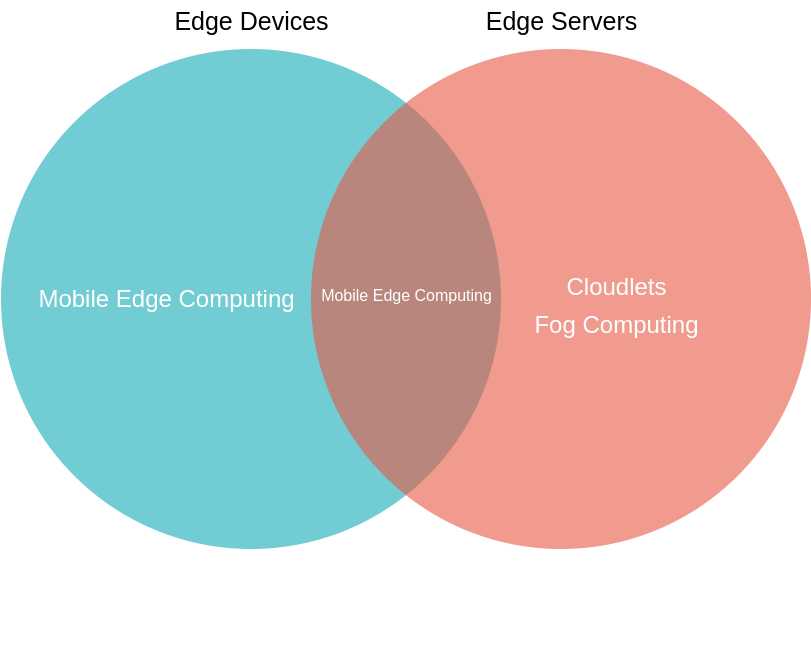
\includegraphics[width = .6\linewidth]{Figures/organization.png}
    \caption{Correspondence to the classifications of edge computing devices and systems from Khan et al. \cite{khan2019edge} and Shi et al. \cite{shi2016promise}}
    \label{fig:organization}
\end{figure}

Regarding a formal Edge AI definition, none of the authors present a formal definition of Edge AI. As much as the definition seems evident at this point, there is no formal sentence defining the concept. For this matter, we establish an entry for the concept of Edge AI.

\begin{itemize}
    \item \textbf{Edge AI Concept:} Edge AI is the set of methods that describes the design process and validation of solutions that combine edge computing and machine learning concepts in developing novel appliances, systems, and applications to solve real-world problems.
\end{itemize}

This definition bases itself on the main common aspects of all evaluated works. It is important to mention that this definition encompasses the other terminologies found in the literature, such as Edge Intelligence, and In-Edge AI, among others. From previous analyses, we also state some of the main features of Edge AI, which are:

\begin{itemize}
    \item Regarding the \textbf{devices' role} in edge computing appliances, the devices can be \textit{edge servers} or \textit{edge devices};
    \item Regarding the \textbf{applications' organization}, an application can be classified among \textit{mobile edge computing}, \textit{fog computing}, and \textit{cloudlets}.
\end{itemize}

We use Edge AI as the official terminology in this work. Nonetheless, it is essential to clarify that this concept and features also refer to works that consider Edge Intelligence or other terminologies, as this is a general terminology. Finally, these terms work regardless of the technologies applied, as long as they can be classified as edge computing and AI together.

\section{Mapping Edge AI applications}
\label{sec:mapping}

After defining the Edge AI, we also provide a mapping of the applications based on this concept. We initially assess and discuss some of the main works regarding Edge AI applications, their organization, and algorithms. Then, we provide some insights on classifying these systems according to the existing organizations and their contexts.

To perform this evaluation, we searched through the bibliography for papers describing applications based on Edge AI. For this matter, we used four different research strings to perform this search, performed on Google Scholar:

\begin{itemize}
    \item ``Edge AI'';
    \item ``Edge Intelligence'';
    \item ``Edge Computing Intelligent System'';
    \item ``Edge AI system'';
\end{itemize}

We initially curated 70 articles describing appliances based on edge computing and AI algorithms. The criteria to select papers was that they should describe one or more case studies that are direct applications of Edge AI. After reviewing this selection, we remained with 54 papers. We excluded those that described general-use frameworks or did not describe specific use cases.

For evaluation purposes, we decided to provide a set of variables to be evaluated considering the edge computing and AI classifications. As discussed in the previous sections, edge computing systems can be classified into three classes according to their organization paradigm: cloudlets, fog computing, or mobile edge computing. Also, the devices running intelligent models can be classified into two main categories: edge devices and edge servers. For the AI, we will initially provide which algorithm or paradigm was used in the appliance. We will also briefly describe the process described in the paper.

\subsection{Applications Overview}

This subsection provides an overview of the applications. Each paragraph describes briefly a single work found in the literature. For each work, we evaluate the system's organization pattern (Mobile Edge, Fog, or Cloudlets), the AI paradigm applied in the solution, and whether the intelligence algorithms run on separate edge servers or edge nodes. The selection and classification criteria are described at the beginning of this section. 

%%%%%%%%%%%%%%%%%%%%%%%%%

The text \textit{iRobot-Factory: An intelligent robot factory based on cognitive manufacturing and edge computing \cite{hu2019irobot}} describes an architecture of a multi-robot factory based on Edge AI. In this case, the edge devices are the robots and sensors involved in the production process. The intelligence algorithms are based on edge servers through direct connection or emulating cloud services. Their application targets the creation of intelligent and integrated industrial architectures.

% \begin{itemize}
%     \item \textbf{Edge computing organization:} Cloudlets;
%     \item \textbf{AI location on edge:} Edge server;
%     \item \textbf{AI paradigms:} Machine Learning, Deep Learning;
% \end{itemize}

%%%%%%%%%%%%%%%%%%%%%%%%%

The work \textit{AI-enabled emotion-aware robot: The fusion of intelligent clothing, edge clouds, and robotics \cite{yang2020ai}} provides a proposal for an application integrating a robot and smart clothing to provide an emotion-aware system to mitigate mental health issues. The involved edge devices, in this case, were wearable devices and robots. Edge server nodes run a system called an emotion-cognition engine to provide AI-based actuation.

% \begin{itemize}
%     \item \textbf{Edge computing organization:} Cloudlets;
%     \item \textbf{AI location on edge:} Edge server;
%     \item \textbf{AI paradigms:} Machine Learning, Deep Learning, Cognitive Computing;
% \end{itemize}

%%%%%%%%%%%%%%%%%%%%%%%%%

The authors of \textit{An edge AI-enabled IoT healthcare monitoring system for smart cities \cite{rathi2021edge}} assess the possibility of creating a healthcare solution based on edge computing, AI, and the IoT. The edge devices involved in this proposal are personal end-users smart devices, patient monitoring devices, and connected ambulances. Intelligent algorithms run on edge servers based in cloudlets.

% \begin{itemize}
%     \item \textbf{Edge computing organization:} Cloudlets;
%     \item \textbf{AI location on edge:} Edge server;
%     \item \textbf{AI paradigms:} Machine Learning, Deep Learning;
% \end{itemize}

%%%%%%%%%%%%%%%%%%%%%%%%%

In \textit{Energy efficient for UAV-enabled mobile edge computing networks: Intelligent task prediction and offloading \cite{wu2020energy}}, the authors provide a network-based application for unmanned aerial vehicles (UAVs) for intelligent tasks. In this work, the edge devices are UAVs, smart devices, and edge servers. The intelligent inferences occur in Edge Servers throughout a mobile edge computing organization. 

% \begin{itemize}
%     \item \textbf{Edge computing organization:} Mobile edge computing;
%     \item \textbf{AI location on edge:} Edge server;
%     \item \textbf{AI paradigms:} Long Short-Term Memory (LSTM)-based prediction, optimization;
% \end{itemize}

%%%%%%%%%%%%%%%%%%%%%%%%%

The work entitled \textit{Real-time strawberry detection using deep neural networks on embedded system (rtsd-net): An edge AI application \cite{zhang2022real}} provides a case study in which the authors apply computer vision and deep neural networks to detect strawberries in real-time. The edge devices involved in this perspective are UAVs and an edge server node. Intelligence algorithms run on the edge server node, provided by the Jetson Nano development board.

% \begin{itemize}
%     \item \textbf{Edge computing organization:} Mobile edge computing;
%     \item \textbf{AI location on edge:} Edge server;
%     \item \textbf{AI paradigms:} Deep Neural Networks (DNNs);
% \end{itemize}

%%%%%%%%%%%%%%%%%%%%%%%%%

In the work named \textit{Edge computing and artificial intelligence for real-time poultry monitoring \cite{debauche2020edge}}, the authors propose and prototype an application for real-time poultry monitoring. The intelligent algorithm runs on a mobile edge computing server based on a Jetson Nano development board. The authors used ESP32 microcontrollers as the media for sensing the environment.

% \begin{itemize}
%     \item \textbf{Edge computing organization:} Mobile edge computing;
%     \item \textbf{AI location on edge:} Edge server;
%     \item \textbf{AI paradigms:} Long Short-Term Memory (LSTM);
% \end{itemize}

%%%%%%%%%%%%%%%%%%%%%%%%%

The text named \textit{Edge AI-IoT pivot irrigation, plant diseases, and pests identification \cite{debauche2020edge-1}} describes the usage of Edge AI within an IoT perspective to detect pests and diseases in plants. They also monitor environmental variables to detect anomalies. In their case, the edge devices are weather stations, remote sensors, and image capturing devices. The edge server runs several intelligent processes to provide insights into understanding environmental health.

% \begin{itemize}
%     \item \textbf{Edge computing organization:} Mobile edge computing;
%     \item \textbf{AI location on edge:} Edge server;
%     \item \textbf{AI paradigms:} Deep Learning;
% \end{itemize}

%%%%%%%%%%%%%%%%%%%%%%%%%

The paper \textit{Edge computing and artificial intelligence for landslides monitoring \cite{elmoulat2020edge}} discusses the possibility of using Wireless Sensor Networks (WSNs), the IoT, and artificial intelligence to monitor landslides. The edge devices involved in the proposed architecture are multiple sensing nodes. The edge servers, in this case, are ODroid N2s and Jetson Nano boards, which run the intelligence algorithms.

% \begin{itemize}
%     \item \textbf{Edge computing organization:} Mobile edge computing;
%     \item \textbf{AI location on edge:} Edge server;
%     \item \textbf{AI paradigms:} Machine Learning;
% \end{itemize}

%%%%%%%%%%%%%%%%%%%%%%%%%

In the article \textit{Edge AI in smart farming IoT: CNNs at the edge and fog computing with LoRa \cite{gia2019edge}} the authors propose an appliance using edge and fog computing to provide Edge AI for smart farming. The edge devices are power-efficient IoT sensors that communicate through LPWAN networks. The intelligence applications are distributed among the fog and cloud layers. 

% \begin{itemize}
%     \item \textbf{Edge computing organization:} Fog computing;
%     \item \textbf{AI location on edge:} Edge server;
%     \item \textbf{AI paradigms:} Long Short-Term Memory (LSTM);
% \end{itemize}

%%%%%%%%%%%%%%%%%%%%%%%%%

In the paper \textit{Edge Intelligence-Assisted Smoke Detection in Foggy Surveillance Environments \cite{muhammad2019edge}}, the authors discuss the training and deployment of an Edge-AI-based system to detect smoke in foggy surveillance environments. The edge intelligence proposed models are convolutional neural networks (CNNs) that classify an image according to the presence of smoke. They search for models with lesser operations per second and size to enable the deployment of edge devices.

% \begin{itemize}
%     \item \textbf{Edge computing organization:} Mobile edge computing;
%     \item \textbf{AI location on edge:} Edge device;
%     \item \textbf{AI paradigms:} Convolutional Neural Networks (CNNs);
% \end{itemize}

%%%%%%%%%%%%%%%%%%%%%%%%%

In the work named \textit{Deep-Learning-Based Visual Odometry Models for Mobile Robotics \cite{de2021deep}}, the authors propose the usage of CNNs and data from a simultaneous localization and mapping (SLAM) data to generate visual odometry models. The edge devices were robots with different capabilities: one can perform slam, while the other relies on visual odometry. The intelligence algorithm runs directly on the edge device.

% \begin{itemize}
%     \item \textbf{Edge computing organization:} Mobile edge computing;
%     \item \textbf{AI location on edge:} Edge device;
%     \item \textbf{AI paradigms:} Convolutional Neural Networks (CNNs);
% \end{itemize}

%%%%%%%%%%%%%%%%%%%%%%%%%

The article \textit{IDiSSC: Edge-computing-based Intelligent Diagnosis Support System for Citrus Inspection \cite{iceis21orange}} presents a proposal of an algorithm to perform the inspection of citrus fruits using Edge AI. The edge devices are image-capturing gear. The authors assess the possibility of using both edge devices or edge server hardware in the disease detection process.

% \begin{itemize}
%     \item \textbf{Edge computing organization:} Mobile edge computing;
%     \item \textbf{AI location on edge:} Edge device or edge server;
%     \item \textbf{AI paradigms:} Machine Learning;
% \end{itemize}

%%%%%%%%%%%%%%%%%%%%%%%%%

In \textit{Conveyor Belt Longitudinal Rip Detection Implementation with Edge AI \cite{Klippel2021}}, the authors assess the proposal of a novel conveyor belt rip detection system using edge AI for the mining industry. The edge devices, in this case, are image-capturing apparatuses. The authors' study considers the possibility of running the intelligence algorithms on both edge devices and edge servers.

% \begin{itemize}
%     \item \textbf{Edge computing organization:} Mobile edge computing;
%     \item \textbf{AI location on edge:} Edge device or edge server;
%     \item \textbf{AI paradigms:} Convolutional Neural Networks (CNNs);
% \end{itemize}

%%%%%%%%%%%%%%%%%%%%%%%%%

The paper \textit{Edge Deep Learning Applied to Granulometric Analysis on Quasi-particles from the Hybrid Pelletized Sinter (HPS) Process \cite{iceis21hps}} discusses a novel proposal for an edge-computing- and AI-based system to detect Quasi-particles in a steel industry process. The edge device involved in this proposal is an image capturing device, which also bears processing capabilities. The intelligence algorithms are CNNs running on the edge device.

% \begin{itemize}
%     \item \textbf{Edge computing organization:} Mobile edge computing;
%     \item \textbf{AI location on edge:} Edge device;
%     \item \textbf{AI paradigms:} Convolutional Neural Networks (CNNs);
% \end{itemize}

%%%%%%%%%%%%%%%%%%%%%%%%%

In the work called \textit{Investigating the Spread of Coronavirus Disease via Edge-AI and Air Pollution Correlation \cite{gomathy2021investigating}}, the authors present an application based on information from an Edge AI system and Air Pollution data to investigate the spread of coronavirus disease. In this case, the authors evaluate the information flow from the cloud to the edge to perform predictions.

% \begin{itemize}
%     \item \textbf{Edge computing organization:} Cloudlets;
%     \item \textbf{AI location on edge:} Edge server;
%     \item \textbf{AI paradigms:} Machine Learning;
% \end{itemize}

%%%%%%%%%%%%%%%%%%%%%%%%%

The paper \textit{A Lossless Data-Hiding based IoT Data Authenticity Model in Edge-AI for Connected Living \cite{rahman2021lossless}} discusses the usage of Edge AI to verify and validate smart living IoT data before passing it through analytics. In this case, the edge devices are local IoT sensor nodes, mainly monitoring the user's health. The intelligent verification algorithm runs on an Edge AI server node.

% \begin{itemize}
%     \item \textbf{Edge computing organization:} Mobile edge computing;
%     \item \textbf{AI location on edge:} Edge server;
%     \item \textbf{AI paradigms:} Ant Colony Optimization;
% \end{itemize}

%%%%%%%%%%%%%%%%%%%%%%%%%

The article \textit{Edge Computing AI-IoT Integrated Energy-Efficient Intelligent Transportation System for Smart Cities \cite{chavhan2022edge}} displays a distributed multi-agent system based on edge computing, AI, and IoT for efficient and intelligent transportation. The intelligence systems run on cloudlets. Edge devices in this network are onboard devices gathering sensor data from transporting agents.

% \begin{itemize}
%     \item \textbf{Edge computing organization:} Cloudlets;
%     \item \textbf{AI location on edge:} Edge server;
%     \item \textbf{AI paradigms:} Stochastic Models, Radial Basis Function Neural Networks;
% \end{itemize}

%%%%%%%%%%%%%%%%%%%%%%%%%

In \textit{National Sports AI Health Management Service System Based on Edge Computing \cite{yang2021national}}, the authors propose an AI sports health management system based on edge computing. Edge devices in this context are smart sensors and intelligent health systems. Intelligence algorithms run in cloudlet layers of the application.

% \begin{itemize}
%     \item \textbf{Edge computing organization:} Cloudlets;
%     \item \textbf{AI location on edge:} Edge server;
%     \item \textbf{AI paradigms:} Query optimization algorithms;
% \end{itemize}

%%%%%%%%%%%%%%%%%%%%%%%%%

The authors of \textit{Towards AI-Based Traffic Counting System with Edge Computing \cite{dinh2021towards}} discuss implementing an AI-based traffic counting system based on the intelligent transportation system concept. The edge devices in this context are cameras capturing live traffic images attached to AI-capable hardware. The edge devices run the intelligence models and feed a server with information.

% \begin{itemize}
%     \item \textbf{Edge computing organization:} Mobile edge computing;
%     \item \textbf{AI location on edge:} Edge device;
%     \item \textbf{AI paradigms:} Convolutional neural networks (CNNs);
% \end{itemize}

%%%%%%%%%%%%%%%%%%%%%%%%%

\textit{Edge AI-Based Automated Detection and Classification of Road Anomalies in VANET Using Deep Learning \cite{bibi2021edge}} discusses the application of DNNs and edge computing to create an intelligent environment for road anomalies detection and classification. Edge devices, in this case, are image-capturing instruments distributed among the network. Edge servers integrate the Vehicular Ad Hoc Network (VANET), running intelligence algorithms.

% \begin{itemize}
%     \item \textbf{Edge computing organization:} Mobile edge computing;
%     \item \textbf{AI location on edge:} Edge server;
%     \item \textbf{AI paradigms:} Deep Neural Networks (DNNs);
% \end{itemize}

%%%%%%%%%%%%%%%%%%%%%%%%%

The work named \textit{Intelligent and Smart Irrigation System Using Edge Computing and IoT \cite{munir2021intelligent}} proposes the intelligent usage of ontology and sensor data together with a machine learning classification algorithm to create a smart irrigation system based on Edge AI. Edge devices are smart sensors capturing field data. Intelligent algorithms run on the edge server layer.

% \begin{itemize}
%     \item \textbf{Edge computing organization:} Mobile edge computing;
%     \item \textbf{AI location on edge:} Edge server;
%     \item \textbf{AI paradigms:} Machine Learning;
% \end{itemize}

%%%%%%%%%%%%%%%%%%%%%%%%%

The paper entitled \textit{AI at the Edge for Sign Language Learning Support \cite{battistoni2019ai}} suggests a novel method to recognize the American Sign Language (ASL) alphabet using CNNs and Fog Computing. Edge devices in this architecture are smart end devices responsible for capturing images. The proposed method deploys the intelligent algorithms on a fog computing layer.

% \begin{itemize}
%     \item \textbf{Edge computing organization:} Fog computing;
%     \item \textbf{AI location on edge:} Edge server;
%     \item \textbf{AI paradigms:} Convolutional Neural Networks (CNNs);
% \end{itemize}

%%%%%%%%%%%%%%%%%%%%%%%%%

In \textit{AI on edge device for laser chip defect detection \cite{hou2019ai}}, the authors propose a novel edge system to detect defects in chips based on laser images. Intelligence algorithms run on the edge device, accelerated by a neural network stick. The edge devices are computer-on-modules with an attached microscope and a neural network accelerator.

% \begin{itemize}
%     \item \textbf{Edge computing organization:} Mobile edge computing;
%     \item \textbf{AI location on edge:} Edge device;
%     \item \textbf{AI paradigms:} Convolutional Neural Networks (CNNs);
% \end{itemize}

%%%%%%%%%%%%%%%%%%%%%%%%%

The work \textit{An AI-edge Platform with Multimodal Wearable Physiological Signals Monitoring Sensors for Affective Computing Applications \cite{yang2020ai-2}} displays a proposal for a novel platform to monitor user's emotions. The edge devices are a set of wearable sensors measuring electroencephalography (EEG), electrocardiography (ECG), and photoplesmiography (PPG). Intelligence algorithms run on an AI/IoT edge server based on FPGA and a RISC-V platform.

% \begin{itemize}
%     \item \textbf{Edge computing organization:} Mobile edge computing;
%     \item \textbf{AI location on edge:} Edge server;
%     \item \textbf{AI paradigms:} Convolutional Neural Networks (CNNs);
% \end{itemize}

%%%%%%%%%%%%%%%%%%%%%%%%%

In \textit{A New Deep Learning-Based Food Recognition System for Dietary Assessment on An Edge Computing Service Infrastructure \cite{liu2017new}}, the authors propose a food recognition system based on edge computing and AI. Edge devices in this proposal are mobile image capturing devices. The intelligent processing happens in a cloudlet layer.

% \begin{itemize}
%     \item \textbf{Edge computing organization:} Cloudlets;
%     \item \textbf{AI location on edge:} Edge server;
%     \item \textbf{AI paradigms:} Convolutional Neural Networks (CNNs);
% \end{itemize}

%%%%%%%%%%%%%%%%%%%%%%%%%

The authors of \textit{Implementation of Pavement Defect Detection System on Edge Computing Platform \cite{lin2021implementation}} present a novel edge computing platform to detect defects in pavements. Edge devices are a composition of cameras and computing modules. Intelligence algorithms run on these specialized modules, which can be computer-on-modules or FPGAs.

% \begin{itemize}
%     \item \textbf{Edge computing organization:} Mobile edge computing;
%     \item \textbf{AI location on edge:} Edge device;
%     \item \textbf{AI paradigms:} Convolutional Neural Networks (CNNs);
% \end{itemize}

%%%%%%%%%%%%%%%%%%%%%%%%%

\textit{Edge-AI-Based Real-Time Automated License Plate Recognition System \cite{lin2022edge}} presents a new license plate recognition system based on Edge AI and IoT. The edge intelligence runs on the device, which has AI accelerators. The edge devices are image-capturing computer-on-modules.

% \begin{itemize}
%     \item \textbf{Edge computing organization:} Mobile edge computing;
%     \item \textbf{AI location on edge:} Edge device;
%     \item \textbf{AI paradigms:} Convolutional Neural Networks (CNNs);
% \end{itemize}

%%%%%%%%%%%%%%%%%%%%%%%%%

In \textit{A Wireless Multi-Channel Capacitive Sensor System for Efficient Glove-Based Gesture Recognition With AI at the Edge \cite{pan2020wireless}}, the authors present a wearable-based edge system for ASL gesture recognition. Their edge device is a wearable system based on capacitive sensors. The edge intelligence runs in the wearable computer-on-module.

% \begin{itemize}
%     \item \textbf{Edge computing organization:} Mobile edge computing;
%     \item \textbf{AI location on edge:} Edge device;
%     \item \textbf{AI paradigms:} Machine Learning;
% \end{itemize}

%%%%%%%%%%%%%%%%%%%%%%%%%

\textit{Blockchain-Based Trust Edge Knowledge Inference of Multi-Robot Systems for Collaborative Tasks \cite{li2021blockchain}} provides a proposal for a blockchain-based system to provide AI inferences in multi-robot systems. Edge devices are robots composing a multi-robot system. Edge servers, in this case, are local Edge AI nodes that run AI inference algorithms.

% \begin{itemize}
%     \item \textbf{Edge computing organization:} Cloudlets;
%     \item \textbf{AI location on edge:} Edge server;
%     \item \textbf{AI paradigms:} Machine Learning;
% \end{itemize}

%%%%%%%%%%%%%%%%%%%%%%%%%

The paper \textit{Deep Learning Models for Magnetic Cardiography Edge Sensors Implementing Noise Processing and Diagnostics \cite{sakib2021deep}} presents an implementation of deep learning models to process noise and aid in diagnostics using magnetic cardiography edge sensors. Edge devices, in this case, are magnetocardiography (MCG) sensors. Signals are processed in a high-performance edge machine as an edge server.

% \begin{itemize}
%     \item \textbf{Edge computing organization:} Cloudlets;
%     \item \textbf{AI location on edge:} Edge server;
%     \item \textbf{AI paradigms:} Deep Learning;
% \end{itemize}

%%%%%%%%%%%%%%%%%%%%%%%%%

In the work \textit{Deep Reinforcement Learning for Collaborative Edge Computing in Vehicular Networks \cite{li2020deep}}, the authors display a mobile edge computing system based on collaborative and decentralized intelligence in vehicular applications. Edge devices are onboard computers in vehicular networks. Edge servers are distributed edge clusters that run the intelligence algorithms.

% \begin{itemize}
%     \item \textbf{Edge computing organization:} Mobile edge computing;
%     \item \textbf{AI location on edge:} Edge server;
%     \item \textbf{AI paradigms:} Convolutional Neural Networks (CNNs);
% \end{itemize}

%%%%%%%%%%%%%%%%%%%%%%%%%

The work named \textit{Development and Validation of an EEG-Based Real-Time Emotion Recognition System Using Edge AI Computing Platform With Convolutional Neural Network System-on-Chip Design \cite{fang2019development}} displays a solution to recognize emotions using electroencephalography (EEG) data. The edge device employed in this system is a field-programmable gate array (FPGA) board. For the edge server, the application uses networking to develop high-level appliances using the inferences from the edge devices.

% \begin{itemize}
%     \item \textbf{Edge computing organization:} Mobile edge computing;
%     \item \textbf{AI location on edge:} Edge device;
%     \item \textbf{AI paradigms:} Convolutional Neural Networks (CNNs);
% \end{itemize}

%%%%%%%%%%%%%%%%%%%%%%%%%

In the article \textit{Distributed Deep Learning Model for Intelligent Video Surveillance Systems with Edge Computing \cite{chen2019distributed}}, the authors propose a novel model for video surveillance systems based on Edge AI. These are two layers of edge servers, organized as a mobile edge computing appliance and getting closer to cloud integration. In this context, the edge devices are video capturing devices.

% \begin{itemize}
%     \item \textbf{Edge computing organization:} Mobile edge computing;
%     \item \textbf{AI location on edge:} Edge device;
%     \item \textbf{AI paradigms:} Convolutional Neural Networks (CNNs) and Long Short-Term Memory (LSTM);
% \end{itemize}

%%%%%%%%%%%%%%%%%%%%%%%%%

\textit{Edge-AI in LoRa-based Health Monitoring: Fall Detection System with Fog Computing and LSTM Recurrent Neural Networks \cite{queralta2019edge}} presents the proposal of an ecosystem based on Edge AI and LPWAN connections toward remote healthcare monitoring. The edge devices are wearable IoT sensors. Edge servers provide the intelligence algorithms necessary to analyze signals and detect falls.

% \begin{itemize}
%     \item \textbf{Edge computing organization:} Fog computing;
%     \item \textbf{AI location on edge:} Edge server;
%     \item \textbf{AI paradigms:} Long Short-Term Memory (LSTM);
% \end{itemize}


%%%%%%%%%%%%%%%%%%%%%%%%%

The article \textit{Edge artificial intelligence for the industrial internet of things applications: an industrial edge intelligence solution \cite{foukalas2021edge}} presented a novel edge-computing-based model for developing intelligent industrial solutions. The edge devices present in this work are industrial end devices performing several tasks. The intelligence models are updated in the edge servers within the federated learning organization.

% \begin{itemize}
%     \item \textbf{Edge computing organization:} Cloudlets;
%     \item \textbf{AI location on edge:} Edge device;
%     \item \textbf{AI paradigms:} Federated Learning;
% \end{itemize}

%%%%%%%%%%%%%%%%%%%%%%%%%

\textit{AI-Aided Individual Emergency Detection System in Edge-Internet of Things Environments \cite{yang2021ai}} displays an innovative individual emergency detection system based on IoT and edge intelligence. The edge devices, in this case, are mobile phones, capturing their sensors' data throughout the usage time. The intelligence models run on edge servers. 

% \begin{itemize}
%     \item \textbf{Edge computing organization:} Mobile edge computing;
%     \item \textbf{AI location on edge:} Edge server;
%     \item \textbf{AI paradigms:} Multi-layer perceptron (MLP), Support vector machine (SVM), Convolutional neural networks (CNNs);
% \end{itemize}

%%%%%%%%%%%%%%%%%%%%%%%%%

In \textit{Economic data analytic AI technique on IoT edge devices for health
monitoring of agriculture machines \cite{gupta2020economic}}, the authors provide a novel integration model for agricultural machines using Edge AI. In their case, the edge devices are agriculture machines (AgMs) producing data from interconnected sensors. Edge servers run in distributed mobile devices which perform inferences using lightweight models.

% \begin{itemize}
%     \item \textbf{Edge computing organization:} Mobile edge computing;
%     \item \textbf{AI location on edge:} Edge server;
%     \item \textbf{AI paradigms:} Artificial neural networks (ANN);
% \end{itemize}

%%%%%%%%%%%%%%%%%%%%%%%%%

In the article named \textit{Intelligent Edge Computing for IoT-Based Energy Management in Smart Cities \cite{liu2019intelligent}}, the authors present a design for an Edge-AI-based energy management system. In their perspective, the edge devices are IoT sensors distributed on the network. Mid-term edge servers provide intelligent services for energy management.

% \begin{itemize}
%     \item \textbf{Edge computing organization:} Cloudlets;
%     \item \textbf{AI location on edge:} Edge server;
%     \item \textbf{AI paradigms:} Deep neural networks (DNN);
% \end{itemize}

%%%%%%%%%%%%%%%%%%%%%%%%%

\textit{Intelligent Search and Find System for Robotic Platform Based on Smart Edge Computing Service \cite{barnawi2020intelligent}} displays a novel edge service to provide intelligent task division algorithms. The edge devices in this perspective are autonomous robots. A base station contains a terminal that provides a self-design intelligence algorithm and interfaces with an operator. 

% \begin{itemize}
%     \item \textbf{Edge computing organization:} Mobile edge computing;
%     \item \textbf{AI location on edge:} Edge server;
%     \item \textbf{AI paradigms:} Traversal Algorithm;
% \end{itemize}

%%%%%%%%%%%%%%%%%%%%%%%%%

In the article named \textit{Intelligent Traffic Accident Detection System Based on Mobile Edge Computing \cite{liao2017intelligent}}, the authors display a traffic accident detection system based on Edge AI. The edge devices within this perspective are smartphones within a mobile edge computing (MEC) network. Mobile edge servers provide the intelligence algorithms as a service.

% \begin{itemize}
%     \item \textbf{Edge computing organization:} Mobile edge computing;
%     \item \textbf{AI location on edge:} Edge server;
%     \item \textbf{AI paradigms:} Deep neural networks (DNN);
% \end{itemize}

%%%%%%%%%%%%%%%%%%%%%%%%%

The authors of \textit{Low-Power HW Accelerator for AI Edge-Computing in Human Activity Recognition Systems \cite{de2020low}} propose an efficient hardware-accelerated system for human activity recognition. The edge device in this context is self-developed hardware to read inertial sensors and processes. The edge intelligence algorithms are hardware accelerated hybrid neural networks.

% \begin{itemize}
%     \item \textbf{Edge computing organization:} Mobile edge computing;
%     \item \textbf{AI location on edge:} Edge device;
%     \item \textbf{AI paradigms:} Hybrid neural networks (HNN);
% \end{itemize}

%%%%%%%%%%%%%%%%%%%%%%%%%

In the article named \textit{pAElla: Edge AI-Based Real-Time Malware Detection in Data Centers \cite{libri2020paella}}, the authors propose a lightweight and scalable solution to monitor the presence of malware in data centers. The intelligence algorithms are designed to run in the edge devices, which feed inferences to an edge server. The edge devices are IoT computer-on-modules based on ARM processors.

% \begin{itemize}
%     \item \textbf{Edge computing organization:} Mobile edge computing;
%     \item \textbf{AI location on edge:} Edge device;
%     \item \textbf{AI paradigms:} Convolutional Neural Networks (CNNs);
% \end{itemize}

%%%%%%%%%%%%%%%%%%%%%%%%%

The paper \textit{Passban IDS: An Intelligent Anomaly-Based Intrusion Detection System for IoT Edge Devices \cite{eskandari2020passban}} displays a novel IoT intrusion detection system (IDS) based on smart edge computing. The edge devices in this context are IoT gateways. Machine learning models on these gateways provide predictions of potentially hazardous packages.

% \begin{itemize}
%     \item \textbf{Edge computing organization:} Mobile edge computing;
%     \item \textbf{AI location on edge:} Edge device;
%     \item \textbf{AI paradigms:} Machine Learning;
% \end{itemize}

%%%%%%%%%%%%%%%%%%%%%%%%%

\textit{Real-Time Apple Detection System Using Embedded Systems With Hardware Accelerators: An Edge AI Application \cite{mazzia2020real}} presents a novel system to detect apples in orchards based on Edge AI devices. For edge devices, the authors propose several solutions based on embedded computers. These computers run intelligent models to detect the apples directly in frames taken from the orchard.

% \begin{itemize}
%     \item \textbf{Edge computing organization:} Mobile edge computing;
%     \item \textbf{AI location on edge:} Edge device;
%     \item \textbf{AI paradigms:} Machine Learning;
% \end{itemize}

%%%%%%%%%%%%%%%%%%%%%%%%%

The paper \textit{Towards the edge intelligence: Robot assistant for the detection and classification of human emotions \cite{sakib2021deep}} provides a novel method to detect and classify human emotions using edge computing. The edge devices, in this case, are a wearable sensor and an Edge AI camera. The intelligence models run on the edge devices, which also feed an assistant robot with information.

% \begin{itemize}
%     \item \textbf{Edge computing organization:} Mobile edge computing;
%     \item \textbf{AI location on edge:} Edge device;
%     \item \textbf{AI paradigms:} Convolutional neural networks (CNNs);
% \end{itemize}

%%%%%%%%%%%%%%%%%%%%%%%%%

With \textit{Innovative Vineyards Environmental Monitoring System Using Deep Edge AI \cite{coppola2021innovative}}, the authors present a solution to monitor vineyards using edge devices with AI capability. Edge devices are computing nodes capable of running AI models and communicating using LoRaWAN. After acquiring data and predicting, the information is gathered and sent to a central prediction system.

% \begin{itemize}
%     \item \textbf{Edge computing organization:} Mobile edge computing;
%     \item \textbf{AI location on edge:} Edge device;
%     \item \textbf{AI paradigms:} Machine Learning;
% \end{itemize}

%%%%%%%%%%%%%%%%%%%%%%%%%

The authors of \textit{AI-doscopist: a real-time deep-learning-based algorithm for localizing polyps in colonoscopy videos with edge computing devices \cite{poon2020ai}} proposed an algorithm to localize polyps in colonoscopy videos through edge devices. The edge intelligence model uses convolutional neural networks to recognize situations of interest in colonoscopy exam videos. Due to the nature of the models, we analyze that a cloudlet architecture is more suitable for this application.

% \begin{itemize}
%     \item \textbf{Edge computing organization:} Cloudlets;
%     \item \textbf{AI location on edge:} Edge server;
%     \item \textbf{AI paradigms:} Convolutional neural networks (CNNs);
% \end{itemize}

%%%%%%%%%%%%%%%%%%%%%%%%%

The researchers responsible for \textit{Wearable IoT Smart-Log Patch: An Edge Computing-Based Bayesian Deep Learning Network System for Multi-Access Physical Monitoring System \cite{manogaran2019wearable}} proposes a system to monitor physical activities based on wearable patches and Edge AI. The edge devices are IoT smart-log patches that gather data from sensing the users' physical conditions and activities. Intelligence models run on local mobile devices or computer applications.

% \begin{itemize}
%     \item \textbf{Edge computing organization:} Mobile edge computing;
%     \item \textbf{AI location on edge:} Edge server;
%     \item \textbf{AI paradigms:} Bayesian deep learning network (BDLN);
% \end{itemize}

%%%%%%%%%%%%%%%%%%%%%%%%%

The authors of \textit{Smart Video Surveillance System Based on Edge Computing \cite{cob2021smart}} provide an innovative surveillance system based on Edge AI. Edge devices are intelligent cameras capable of running AI models. Intelligence models run on specialized edge hardware that enables running AI models.

% \begin{itemize}
%     \item \textbf{Edge computing organization:} Mobile edge computing;
%     \item \textbf{AI location on edge:} Edge device;
%     \item \textbf{AI paradigms:} Convolutional neural networks (CNNs);
% \end{itemize}

%%%%%%%%%%%%%%%%%%%%%%%%%

In the research named \textit{Wearable Edge AI Applications for Ecological Environments \cite{silva2021wearable}}, the authors provided a novel method to identify diseases in plants and evaluate the spread within canopies. The edge devices, in this case, are smart helmets with IoT capabilities. The intelligence models run on edge servers from a mobile edge computing perspective.

% \begin{itemize}
%     \item \textbf{Edge computing organization:} Mobile edge computing;
%     \item \textbf{AI location on edge:} Edge server;
%     \item \textbf{AI paradigms:} Convolutional neural networks (CNNs), Evolutive Algorithm (EA);
% \end{itemize}

%%%%%%%%%%%%%%%%%%%%%%%%%

The authors of \textit{Deep Learning Approach at the Edge to Detect Iron Ore Type \cite{klippel2021deep}} display a new system based on intelligent sensors to monitor ore types in conveyor belts. The edge devices, in this case, are sensors integrated into the industrial plant with AI capabilities. The intelligence models run within the smart sensors, enabling instant actuation given the test results.

% \begin{itemize}
%     \item \textbf{Edge computing organization:} Mobile edge computing;
%     \item \textbf{AI location on edge:} Edge device;
%     \item \textbf{AI paradigms:} Convolutional neural networks (CNNs);
% \end{itemize}

%%%%%%%%%%%%%%%%%%%%%%%%%

\textit{Green Citrus Detection and Counting in Orchards Based on YOLOv5-CS and AI Edge System \cite{lyu2022green}} displays a new method to detect green citrus in orchards based on Edge AI. The edge device in this proposal is an AI-capable edge computer with a camera to capture images. The models run on the edge device, recognizing green citrus among the orchard.

% \begin{itemize}
%     \item \textbf{Edge computing organization:} Mobile edge computing;
%     \item \textbf{AI location on edge:} Edge device;
%     \item \textbf{AI paradigms:} Convolutional neural networks (CNNs);
% \end{itemize}

%%%%%%%%%%%%%%%%%%%%%%%%%

In \textit{An Edge Intelligence Empowered Recommender System Enabling Cultural Heritage Applications \cite{su2019edge}}, the authors present a new recommendation system based on user information and Edge AI. Edge intelligence allows personalized recommendations based on the users' inputs. The edge devices in this perspective are mobile phones.

% \begin{itemize}
%     \item \textbf{Edge computing organization:} Mobile edge computing;
%     \item \textbf{AI location on edge:} Edge device;
%     \item \textbf{AI paradigms:} Naive Bayes classifier, Europeana Data Model (EDM);
% \end{itemize}

%%%%%%%%%%%%%%%%%%%%%%%%%

In the work \textit{A semi-supervised learning approach for network anomaly detection in fog computing \cite{xu2019semi}}, the authors propose using a Support Vector Machine (SVM) through semi-supervised learning to detect anomalies in the network data flow. The intelligence model, in this case, is a One-Class Support Vector Machine (OCSVM). The semi-supervised learning happens in edge servers, forming a Fog Computing infrastructure.

% \begin{itemize}
%     \item \textbf{Edge computing organization:} Fog computing;
%     \item \textbf{AI location on edge:} Edge server;
%     \item \textbf{AI paradigms:} Support Vector Machine (SVM);
% \end{itemize}

\subsection{Preliminary Analyses}

\begin{figure}[h!]
    \centering
    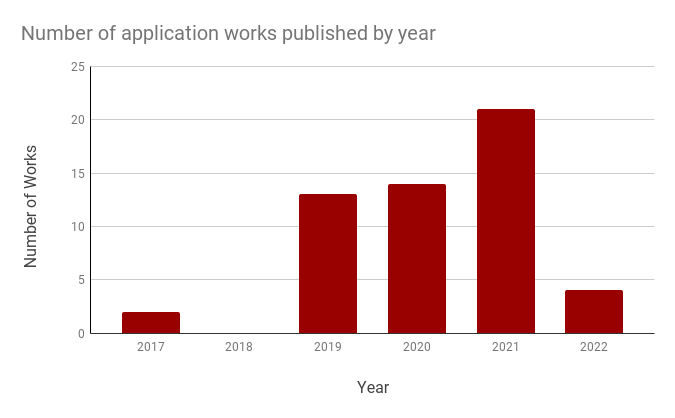
\includegraphics[width = .8\linewidth]{Figures/appl-year.png}
    \caption{Number of application papers per year. The first applications in this context were proposed in 2017, but the it was established in 2019.}
    \label{fig:appyear}
\end{figure}

After studying the works in the literature, we provide an initial overview of some information extracted from the collected data. This information aims to surround the main common aspects of the studied works. Initially, we provide an overview of how many papers were found each year. Figure \ref{fig:appyear} displays the results of this analysis.

From this result, we can initially state that the preliminary works that apply Edge AI concepts came from 2017. Nevertheless, the data indicate that the concept was actually established in 2019. After this year, the number of novel proposed applications is consistent and increased in 2021. Some Edge AI papers were already found in the first quarter of 2022.

\begin{figure}[h!]
    \centering
    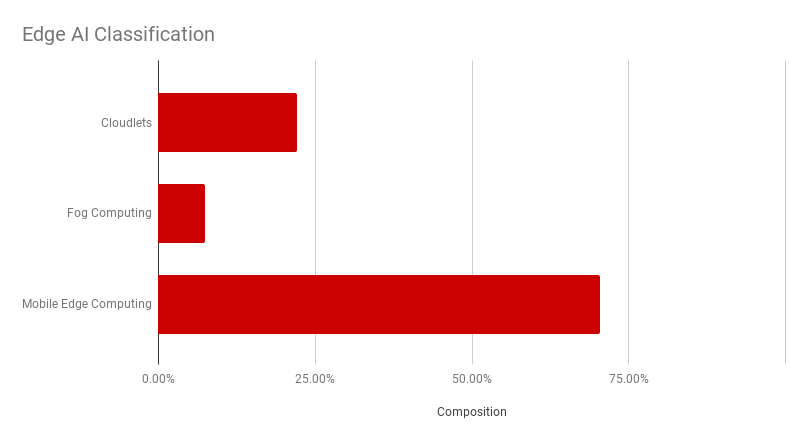
\includegraphics[width = \linewidth]{Figures/edge-classification.png}
    \caption{Contributions of each category of edge computing to the curated appliances. The majority of works apply ``Mobile edge computing''.}
    \label{fig:edgeclass}
\end{figure}

A second relevant analysis regards the edge computing classification. This section classified the works among ``Mobile edge computing'', ``Fog computing'', and ``Cloudlets''. Of the 54 curated articles, 38 applications used Mobile edge computing, 12 used Cloudlets, and four applied Fog computing. Figure \ref{fig:edgeclass} displays the classification data analysis in proportions.

\begin{figure}[h!]
    \centering
    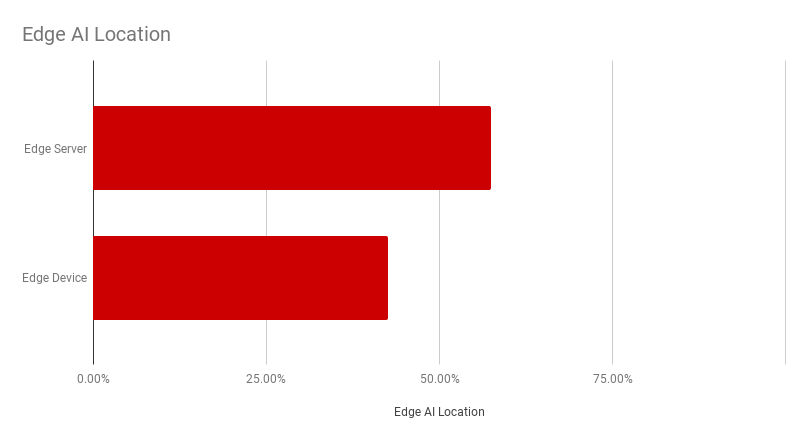
\includegraphics[width = \linewidth]{Figures/location-ai.png}
    \caption{Location of the AI algorithms. The analysis display that appliances can deploy models on edge devices or edge servers.}
    \label{fig:ailocation}
\end{figure}

Another feasible study is whether the appliances run the models in the edge devices or edge servers, according to our preliminary classification. A few more works deployed AI models on edge servers than edge devices. Nonetheless, the data is almost balanced, displaying circa 57\% of the works with AI deployed on edge servers and 43\% on edge devices. In this case, the two works that could run on both devices and servers were classified as ``Edge Device''. Figure \ref{fig:ailocation} displays these results.

\begin{figure}[h!]
    \centering
    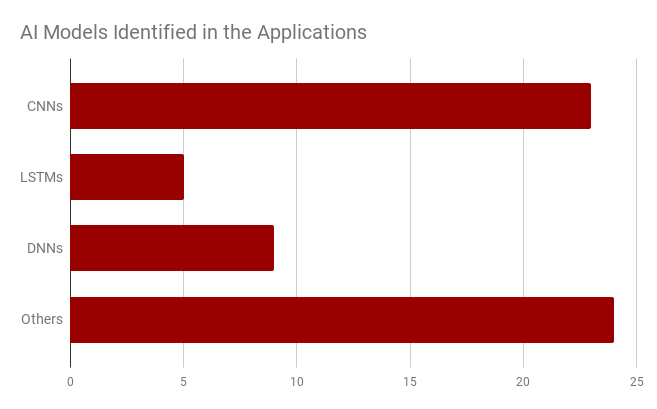
\includegraphics[width = .8\linewidth]{Figures/ai-models.png}
    \caption{AI models identified in the articles. The three individual categories that contributed the most are CNNs, LSTMs, and DNNs. Many authors identify their appliances generically as ``Machine Learning''}
    \label{fig:aimodels}
\end{figure}

Finally, we assess the models used in the studied applications. After inspecting the works initially, we decided to classify the applications among the following classes: \textbf{CNNs}, \textbf{LSTMs}, \textbf{DNNs}, and \textbf{Others/Unspecified}. The three initial classes represent the most models which were individually identified in the papers found in the literature, while the last one treats the exceptions. If a system employs more than one algorithm, all models contribute individually to the count. The results, displayed in Figure \ref{fig:aimodels}, show that CNNs are the most popular models among Edge AI applications. Also, many authors did not specify the machine learning models applied, focusing their papers on the edge computing architecture. DNNs and LSTMs had relevant individual contributions to these numbers.


%%%%%%%%%%%%%%%%%%%%%%%%%%%%%%%%%%%%%%%%%%%%%%%
\section{Edge Computing and AI taxonomies analysis}
\label{sec:taxonomiesanalysis}

After analyzing several applications, the next stage in this research is to understand how the foundation areas are organized. For this matter, we provide a study of the taxonomies in both edge computing and AI means. After this stage, we expect to extract enough information to propose an Edge AI taxonomy.

\subsection{Edge Computing Taxonomies}

Initially, we explored a few works regarding edge computing taxonomies. Finding general information in edge computing taxonomies was not easy, as most texts are focused on single areas or applications. For instance, Beck et al. \cite{beck2014mobile} focus on examining the taxonomy of mobile edge computing solutions. While his work is extensive, it refers to one single of the three main areas of Edge Computing. Thus, this work does not provide a general view of the area.

Regarding a general view of edge computing, Ahmed et al. \cite{ahmed2017bringing} display a comprehensive taxonomy of information that defines edge computing. An essential aspect of this taxonomy within the context of this work is that the authors also evaluate the same computing paradigms as presented by Khan et al. \cite{khan2019edge}, which were one of the bases of this study. The authors also generally classify the technologies among edge devices and edge servers, later using their taxonomy to evaluate the most critical enabling technologies for edge computing.

Dolui and Datta \cite{dolui2017comparison} also use the same three paradigms to classify edge computing applications. These three paradigms work as a baseline to understand the nodes' organization, nodes location, software architecture, context awareness, geographical proximity, access, and communication. This result reinforces the usage of these three paradigms as the general line to classify edge computing applications.

The analysis of these studies, combined with the previous evaluations, leads to the conclusion that a set of technologies based on edge computing should be initially evaluated according to the three computing paradigms that compose the area. The separation among cloudlets, fog computing, and mobile edge computing allows a general classification of the solutions, leading further to the AI classification.

\subsection{AI Algorithms Taxonomies}

The ways of classifying AI are broader than edge computing. For instance, Sheth et al. \cite{sheth2020taxonomy} classify AI according to the learning paradigm (supervised learning, unsupervised learning, reinforcement learning). While we understand that this will later be important to evaluate Edge AI techniques, we search for a broader classification within this work. Another example of this specificity happens in Baltru{\v{s}}aitis, Ahuja, and Morency \cite{baltruvsaitis2018multimodal}. These authors create a taxonomy of specific deep learning relevant within the Multimodal Machine Learning context.

Similarly, Talbi \cite{talbi2021machine} divides AI works according to the algorithms. They provide this classification in the context of evaluating how these algorithms can support metaheuristics. From this work, we understand that using the algorithm paradigms to classify these works is an interesting way of approaching the problem. Still, the way to perform this classification depends on the objective of the algorithms. After searching and evaluating works, we understand that the taxonomy within the AI context should consider the specificity of the desired tasks and concepts. 

\section{Edge AI Taxonomy}
\label{sec:taxonomy}

\begin{figure*}[ht!]
    \centering
    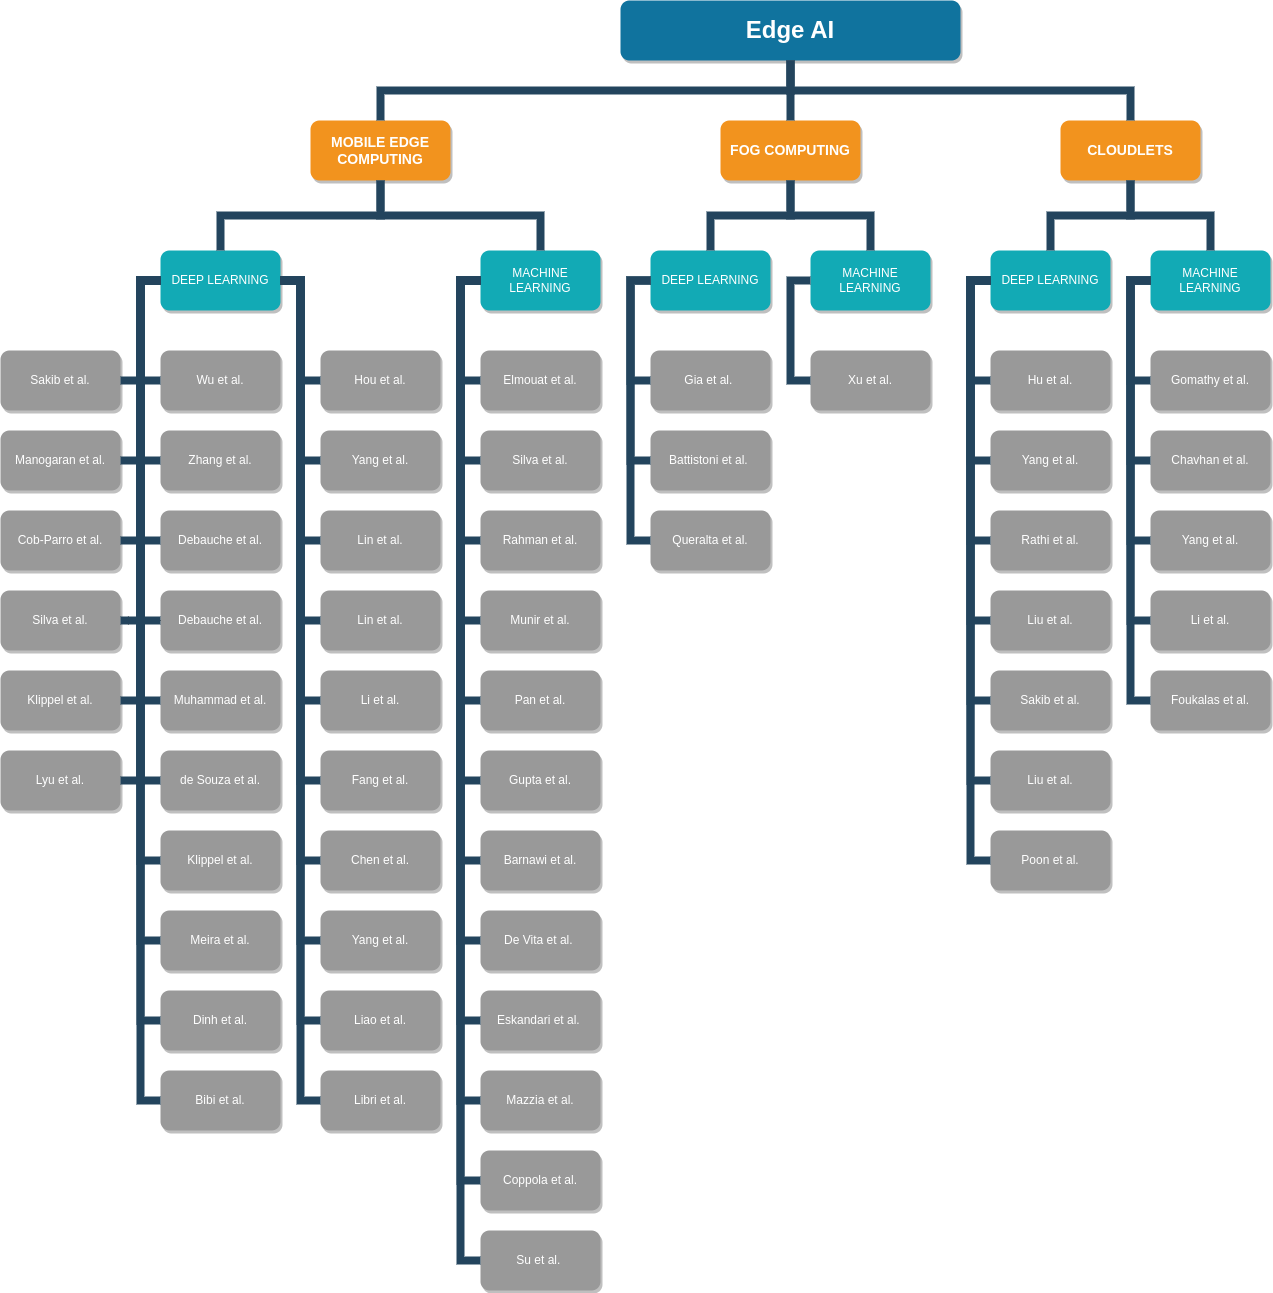
\includegraphics[width=\linewidth]{Figures/taxonomy.png}
    \caption{Classification of the works from Section \ref{sec:mapping} according to the proposed taxonomy. Each gray square is a single work evaluated in this section of the work.}
    \label{fig:taxonomy}
\end{figure*}

Given the knowledge built up to this point, we extracted enough information to propose a new taxonomy to classify Edge AI works and applications. Initially, we start with the edge computing domain, classifying the application among its classes. Then, we evaluate the application according to the AI domain.

The reviews indicate that the classification among the three main classes is adopted for the edge computing traits in both application works and taxonomies. Thus, the first layer of the Edge AI taxonomy evaluates if the works belong to \textit{mobile edge computing}, \textit{fog computing} or \textit{cloudlets} domains. This separation is efficient for dividing edge computing works while separating among edge devices or edge servers only makes sense within \textit{mobile edge computing} domain.

In the AI computing features, we initially observed several ways to separate AI algorithms. Thus, interpreting the data obtained in Section \ref{sec:mapping} was the critical aspect of defining this division. In Figure \ref{fig:aimodels}, we observe that most works use CNNs, LSTMs, or DNNs as the basis of the application. These models belong to the deep learning domain. A similar proportion of works employ other machine learning models or paradigms to employ AI on edge. Thus, we defined two classes: \textit{deep learning}, containing the applications that employ algorithms belonging to the deep learning domain, and \textit{machine learning}, encompassing the applications that employ other methods and paradigms.

In Figure \ref{fig:taxonomy}, we display the reclassification of the works presented in Section \ref{sec:mapping} according to the proposed taxonomy. We manually evaluated each work in this section according to the proposed divisions. If the works employ methods from more than one domain, including deep learning, we consider them to belong to the \textit{deep learning} classes.

What we observe in this case is that the proportions indicate by Figures \ref{fig:edgeclass}, \ref{fig:ailocation}, and \ref{fig:aimodels} were reflected in this taxonomy. Most of the works from Edge AI belong to the \textit{mobile edge computing} domain. Also, most employ algorithms belonging to the \textit{deep learning} domain. The fewest amount of applications was found regarding the \textit{fog computing} domain, while a reasonable amount was found regarding the \textit{cloudlets} domain, with a more balanced division between \textit{deep learning} and \textit{machine learning}.

Finally, we organized a taxonomic table of the displayed works for a better understanding. In Table \ref{tab:taxonomic-table}, we compiled the results displayed through Figure \ref{fig:taxonomy}. This information complements what we presented previously, working as a catalog to find works related to each area.


% Please add the following required packages to your document preamble:
% \usepackage{graphicx}
\begin{table}[h!]
\centering
\caption{Taxonomic table compiling the collected information from papers.}
\label{tab:taxonomic-table}
\resizebox{\textwidth}{!}{%
\begin{tabular}{lll}
\hline
\textbf{Paper Title} & \textbf{Edge Computing Paradigm} & \textbf{AI Paradigm} \\ \hline
Energy efficient for UAV-enabled mobile edge computing networks: Intelligent task prediction and offloading \cite{wu2020energy} & Mobile Edge Computing & Deep Learning \\
Real-time strawberry detection using deep neural networks on embedded system (rtsd-net): An edge AI application \cite{zhang2022real} & Mobile Edge Computing & Deep Learning \\
Edge computing and artificial intelligence for real-time poultry monitoring \cite{debauche2020edge} & Mobile Edge Computing & Deep Learning \\
Edge AI-IoT pivot irrigation, plant diseases, and pests identification \cite{debauche2020edge-1} & Mobile Edge Computing & Deep Learning \\
Edge Intelligence-Assisted Smoke Detection in Foggy Surveillance Environments \cite{muhammad2019edge} & Mobile Edge Computing & Deep Learning \\
Deep-Learning-Based Visual Odometry Models for Mobile Robotics \cite{de2021deep} & Mobile Edge Computing & Deep Learning \\
Conveyor Belt Longitudinal Rip Detection Implementation with Edge AI \cite{Klippel2021} & Mobile Edge Computing & Deep Learning \\
Edge Deep Learning Applied to Granulometric Analysis on Quasi-particles from the Hybrid Pelletized Sinter (HPS) Process \cite{iceis21hps} & Mobile Edge Computing & Deep Learning \\
Towards AI-Based Traffic Counting System with Edge Computing \cite{dinh2021towards} & Mobile Edge Computing & Deep Learning \\
Edge AI-Based Automated Detection and Classification of Road Anomalies in VANET Using Deep Learning \cite{bibi2021edge} & Mobile Edge Computing & Deep Learning \\
AI on edge device for laser chip defect detection \cite{hou2019ai} & Mobile Edge Computing & Deep Learning \\
An AI-edge Platform with Multimodal Wearable Physiological Signals Monitoring Sensors for Affective Computing Applications \cite{yang2020ai-2} & Mobile Edge Computing & Deep Learning \\
Implementation of Pavement Defect Detection System on Edge Computing Platform \cite{lin2021implementation} & Mobile Edge Computing & Deep Learning \\
Edge-AI-Based Real-Time Automated License Plate Recognition System \cite{lin2022edge} & Mobile Edge Computing & Deep Learning \\
Blockchain-Based Trust Edge Knowledge Inference of Multi-Robot Systems for Collaborative Tasks \cite{li2021blockchain} & Mobile Edge Computing & Deep Learning \\
\begin{tabular}[c]{@{}l@{}}Development and Validation of an EEG-Based Real-Time Emotion Recognition System Using Edge AI Computing Platform \\ With Convolutional Neural Network System-on-Chip Design \cite{fang2019development}\end{tabular} & Mobile Edge Computing & Deep Learning \\
Distributed Deep Learning Model for Intelligent Video Surveillance Systems with Edge Computing \cite{chen2019distributed} & Mobile Edge Computing & Deep Learning \\
AI-Aided Individual Emergency Detection System in Edge-Internet of Things Environments \cite{yang2021ai} & Mobile Edge Computing & Deep Learning \\
Intelligent Traffic Accident Detection System Based on Mobile Edge Computing \cite{liao2017intelligent} & Mobile Edge Computing & Deep Learning \\
pAElla: Edge AI-Based Real-Time Malware Detection in Data Centers \cite{libri2020paella} & Mobile Edge Computing & Deep Learning \\
Towards the edge intelligence: Robot assistant for the detection and  classification of human emotions \cite{sakib2021deep} & Mobile Edge Computing & Deep Learning \\
\begin{tabular}[c]{@{}l@{}}Wearable IoT Smart-Log Patch: An Edge Computing-Based Bayesian Deep Learning Network System\\ for Multi Access Physical Monitoring System \cite{manogaran2019wearable}\end{tabular} & Mobile Edge Computing & Deep Learning \\
Smart Video Surveillance System Based on Edge Computing \cite{cob2021smart} & Mobile Edge Computing & Deep Learning \\
Wearable Edge AI Applications for Ecological Environments \cite{silva2021wearable} & Mobile Edge Computing & Deep Learning \\
Deep Learning Approach at the Edge to Detect Iron Ore Type \cite{klippel2021deep} & Mobile Edge Computing & Deep Learning \\
Green Citrus Detection and Counting in Orchards Based on YOLOv5-CS and AI Edge System \cite{lyu2022green} & Mobile Edge Computing & Deep Learning \\ \hline
Edge computing and artificial intelligence for landslides monitoring \cite{elmoulat2020edge} & Mobile Edge Computing & Machine Learning \\
IDiSSC: Edge-computing-based Intelligent Diagnosis Support System for Citrus Inspection \cite{iceis21orange} & Mobile Edge Computing & Machine Learning \\
A Lossless Data-Hiding based IoT Data Authenticity Model in Edge-AI for Connected Living \cite{rahman2021lossless} & Mobile Edge Computing & Machine Learning \\
Intelligent and Smart Irrigation System Using Edge Computing and IoT \cite{munir2021intelligent} & Mobile Edge Computing & Machine Learning \\
A Wireless Multi-Channel Capacitive Sensor System for Efficient Glove-Based Gesture Recognition With AI at the Edge \cite{pan2020wireless} & Mobile Edge Computing & Machine Learning \\
Economic data analytic AI technique on IoT edge devices for health monitoring of agriculture machines \cite{gupta2020economic} & Mobile Edge Computing & Machine Learning \\
Intelligent Search and Find System for Robotic Platform Based on Smart Edge Computing Service \cite{barnawi2020intelligent} & Mobile Edge Computing & Machine Learning \\
Low-Power HW Accelerator for AI Edge-Computing in Human Activity Recognition Systems \cite{de2020low} & Mobile Edge Computing & Machine Learning \\
Passban IDS: An Intelligent Anomaly-Based Intrusion Detection System for IoT Edge Devices \cite{eskandari2020passban} & Mobile Edge Computing & Machine Learning \\
Real-Time Apple Detection System Using Embedded Systems With Hardware Accelerators: An Edge AI Application \cite{mazzia2020real} & Mobile Edge Computing & Machine Learning \\
Innovative Vineyards Environmental Monitoring System Using Deep Edge AI \cite{coppola2021innovative} & Mobile Edge Computing & Machine Learning \\
An Edge Intelligence Empowered Recommender System Enabling Cultural Heritage Applications \cite{su2019edge} & Mobile Edge Computing & Machine Learning \\ \hline
Edge AI in smart farming IoT: CNNs at the edge and fog computing with LoRa \cite{gia2019edge} & Fog Computing & Deep Learning \\
AI at the Edge for Sign Language Learning Support \cite{battistoni2019ai} & Fog Computing & Deep Learning \\
Edge-AI in LoRa-based Health Monitoring: Fall Detection System with Fog Computing and LSTM Recurrent Neural Networks \cite{queralta2019edge} & Fog Computing & Deep Learning \\ \hline
A semi-supervised learning approach for network anomaly detection in fog computing \cite{xu2019semi} & Fog Computing & Machine Learning \\ \hline
iRobot-Factory: An intelligent robot factory based on cognitive manufacturing and edge computing \cite{hu2019irobot} & Cloudlets & Deep Learning \\
AI-enabled emotion-aware robot: The fusion of smart clothing, edge clouds and robotics \cite{yang2020ai} & Cloudlets & Deep Learning \\
An edge AI-enabled IoT healthcare monitoring system for smart cities \cite{rathi2021edge} & Cloudlets & Deep Learning \\
A New Deep Learning-Based Food Recognition System for Dietary Assessment on  An Edge Computing Service Infrastructure \cite{liu2017new} & Cloudlets & Deep Learning \\
Deep Learning Models for Magnetic Cardiography Edge Sensors Implementing Noise Processing and Diagnostics \cite{sakib2021deep} & Cloudlets & Deep Learning \\
Intelligent Edge Computing for IoT-Based Energy Management in Smart Cities \cite{liu2019intelligent} & Cloudlets & Deep Learning \\
AI-doscopist: a real-time deep-learning-based algorithm for localising polyps in colonoscopy videos with edge computing devices \cite{poon2020ai} & Cloudlets & Deep Learning \\ \hline
Investigating the Spread of Coronavirus Disease via Edge-AI and Air Pollution Correlation \cite{gomathy2021investigating} & Cloudlets & Machine Learning \\
Edge Computing AI-IoT Integrated Energy Efficient Intelligent Transportation System for Smart Cities \cite{chavhan2022edge} & Cloudlets & Machine Learning \\
National Sports AI Health Management Service System Based on Edge Computing \cite{yang2021national} & Cloudlets & Machine Learning \\
Blockchain-Based Trust Edge Knowledge Inference of Multi-Robot Systems for Collaborative Tasks \cite{li2021blockchain} & Cloudlets & Machine Learning \\
Edge artificial intelligence for industrial internet of things applications: an industrial edge intelligence solution \cite{foukalas2021edge} & Cloudlets & Machine Learning \\ \hline
\end{tabular}%
}
\end{table}

% \section{Future Trends in Edge AI}
% \label{sec:futuretrends}

% After discussing the concept and classifications of Edge AI, we also provide this space with an overview of some areas that might contribute to this area's development. From our research, we understand that some critical issues connected to the future of Edge AI are 5G, 6G, Blockchain, and Federated Learning \cite{sheth2020taxonomy,fantacci2020federated,wang2019edge,nguyen2021federated,al2021survey}.

% \subsection{Edge AI, 5G, and 6G}

% 5G and 6G are the most current communication standards for broadband and wireless communications. Chowdhury et al. \cite{chowdhury2019role} state that the uprise of these technologies will enhance IoT-based solutions. Towards this aspect, Lovén et al. \cite{loven2019edgeai} envision the reduced latency of upcoming 5G and 6G networks as fundamental aspects in developing Edge AI applications. Xiao et al. \cite{xiao2020toward} present Edge AI as the missing link in the 5G communication paradigm. Furthermore, they assert that these technologies will have an essential role in implementing future 6G networks. Thus, they also recognize the importance of these technologies to future research involving these new communication paradigms. 5G and 6G present a substantial interest field to be considered when proposing novel applications involving Edge AI.

% \subsection{Edge AI in Blockchain}

% Blockchain is a composition using a set of technologies to provide secure transactions. Initially, it was developed towards cryptocurrencies, but its application raised as many processes require secure information storage and authentic transactions \cite{di2017blockchain}. This technology integrates well with some concepts within the Edge AI domain. It can be applied to improving mining and data processing in mobile edge computing, resource allocation in IoT/mobile edge computing, and content caching in vehicular networks \cite{qiu2019online,he2020blockchain,dai2020deep}, among others. Nguyen et al. \cite{nguyen2021federated} even explore its integration with the next paradigm, federated learning, within the context of mobile edge computing. These works display that integrating blockchain and Edge AI is a large field to explore in future implementations.

% \subsection{Edge AI in Federated Learning}

% Federated learning is an approach to distributing machine learning among devices within a network \cite{bonawitz2019towards}. This precedent is interesting within edge computing, where we expect to distribute computational charges among devices within a network. Some authors explore the possibility of reducing the computing offload or optimizing the training process by considering a federated learning approach \cite{wang2019adaptive,wang2019edge,ye2020edgefed,yu2021toward}. Others suggest fields of employment as vehicular networks and mobile edge computing \cite{ye2020federated,fantacci2020federated,lu2019differentially}. This perspective indicates that this area should also be explored for further implementations in future perspectives.

\section{Final Remarks}
\label{sec:conclusions}

Edge computing and artificial intelligence initially had conflicting requirements. As AI required more processing throughout time, edge computing developed mainly over hardware miniaturization and increased mobility. Nevertheless, a recent trend displayed increasing applications applying both concepts together, especially in mobile edge computing. Although other research papers survey functional aspects \cite{mendez2022edge}, applications for specific areas \cite{amin2020edge}, or even specific technologies \cite{lalapura2021recurrent}, the area lacks a general conceptualization and taxonomy.

This trend had several names up to this moment, but every one of them had similar premises of uniting edge computing with AI algorithms. Moreover, a significant number of papers describing applications in this context were published from 2019 on. To define this area, we started from the fundamental areas behind the appliances: edge computing and AI. We named this novel concept Edge AI, one of the names used to describe these appliances in the literature. 

Edge computing is divided into three main areas: cloudlets, fog computing, and mobile edge computing. Cloudlets refer to resourceful infrastructures built to provide AI closer to the end-user. Fog computing regards the distribution among heterogeneous devices and the virtualization of cloud-like services. Mobile edge computing describes more mobile and isolated infrastructure, where less powerful devices and more restricted resources are employed to provide AI.

AI can be divided in many ways. Mainly, it refers to machine learning processes where algorithms learn to solve a task from provided data. The more modern applications of machine learning are described in the literature as deep learning, having several specific algorithms in this domain. Within edge computing, AI can run in single-edge devices or as a service in edge servers. The first mode is only referred to in the mobile edge computing domain.

This information helped us create a taxonomy to classify applications described in papers from the literature. The works can belong to three edge domains: cloudlets, fog computing, and mobile edge computing. The first layer evaluates the edge computing classification. The second layer divides the AI among the deep learning domain or belonging to any other paradigm of AI. 

Finally, some of the main future trends regarding Edge AI integrate concepts like Blockchain, 5G, 6G, and Federated Learning \cite{sheth2020taxonomy,fantacci2020federated,wang2019edge,nguyen2021federated,al2021survey}. Future works can explore these aspects as the ground for further investigation. Also, as mobile edge computing contains the most developed area among these domains within Edge AI, it requires further investigations and classifications on its own, possibly as a ``Mobile Edge AI'' concept.

\cleardoublepage
  \chapter{Wearable Edge AI}
\label{chap:wearable-edge-ai}

\nomenclature{CPU}{Central Processing Unit}
\nomenclature{PCB}{Printed Circuit Board}
\nomenclature{WBAN}{Wireless Body-Area Network}

\begin{figure}[h!]
    \centering
    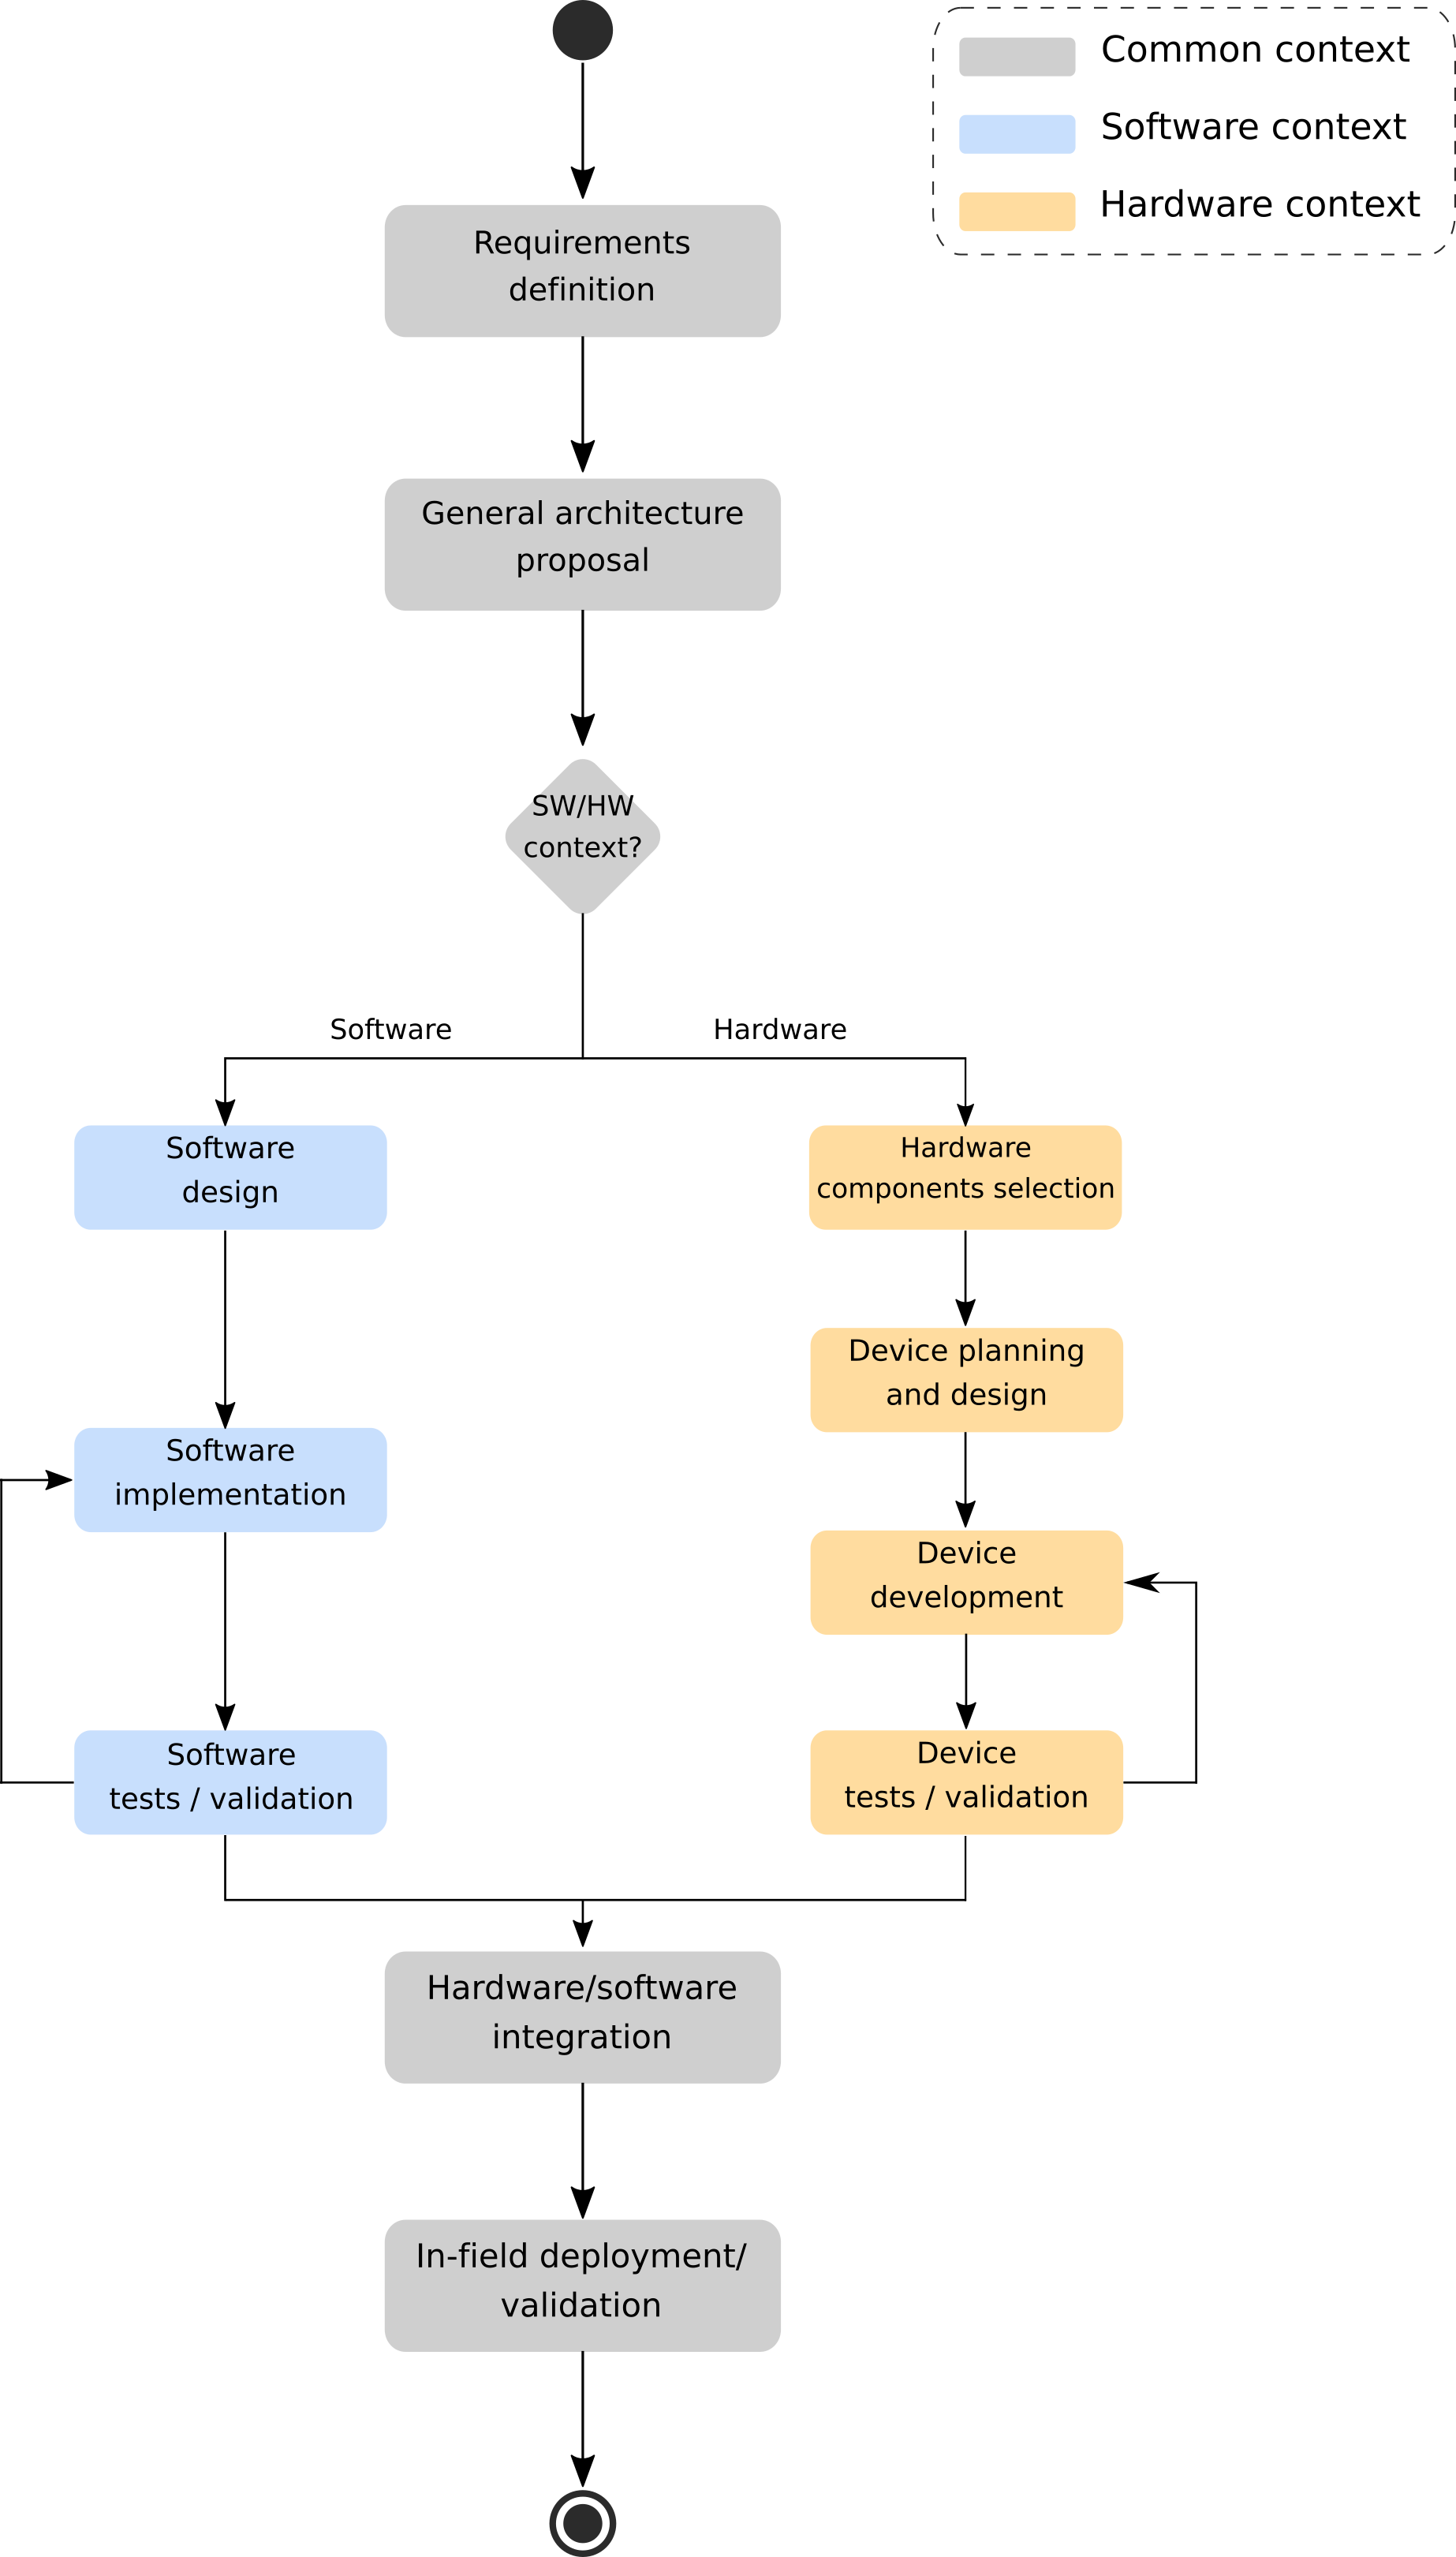
\includegraphics[width = .5\linewidth]{Figures/design_diagram.png}
    \caption{Original Hardware and Software co-design process, presented in \cite{silva2019field}}
    \label{fig:hw-sw-codesign}
\end{figure}

This chapter discusses the creation of the \textit{Wearable Edge AI} concept. Our discussion begins with an understanding of how cooperative wearable systems work. Then, we review the hardware/software co-design process. Finally, we assess the wearable edge AI concept, surrounding its constraints and its creation and validation processes.

Our concept starts from the wearable systems perspective. Thus, it is required to understand the design process behind them. As an inheritance from their embedded systems' origin, wearable devices and systems usually follow a process known as hardware and software co-design \cite{silva2019field}, exemplified in Figure \ref{fig:hw-sw-codesign}. 

As displayed, a series of steps are required to produce these solutions. Initially, there are two general steps to start projecting these appliances:

\begin{itemize}
    \item \textbf{Requirements definition:} This stage involves collecting, assessing, and examining the system requirements. This is achieved by conducting a thorough analysis of the stakeholders' needs;
    
    \item \textbf{General architecture proposal:} During this stage, professionals utilize the data collected from the previous step to create a preliminary outline of the proposal. This initial blueprint necessitates defining the limitations for both software and hardware to strategize the flow of information.
\end{itemize}

Following these preliminary stages, there are several simultaneous activities related to the software and hardware characteristics. These steps occur concurrently since their outcomes are interdependent. They are:

\begin{itemize}
    \item \textbf{Hardware:} 
    \begin{itemize}
        \item \textbf{Hardware components selection:} The initial step in the hardware phase is to list the necessary hardware components required to execute the proposed tasks and functions.
        \item \textbf{Prototype planning and design:} Hardware components act as input data for devising and developing the final prototype. During this stage, connections between components are specified, and if required, the Printed Circuit Board (PCB) layout is outlined;
        \item \textbf{Prototype development:} This phase involves the production of the wearable device. The primary Central Processing Unit (CPU) and hardware peripheral components are physically linked, potentially employing the final version of the PCBs created in the previous stage. Finally, the components can be attached to the garment;
        \item \textbf{Device tests/validation:} Multiple rounds of on-site hardware testing and validation are conducted to authenticate the connections established with each component. If any issues arise during this stage, they can be rectified or altered in a new development round.
    \end{itemize}
    \item \textbf{Software:}
    \begin{itemize}
        \item \textbf{Software design:} The previously stated requirements can also serve as a guide for devising the relevant software. This phase entails defining functionalities and how internal modules will communicate with one another;
        \item \textbf{Software implementation:} The design created earlier can now be utilized as a point of reference for precisely coding the software. Typically, specific and lightweight programming languages/frameworks can be employed during this stage, depending on the requirements of the entire solution;
        \item \textbf{Software tests/validation:} This module is responsible for testing and verifying whether the resultant software adheres to the previously stated requirements. If the solution fails to meet the necessary requirements or does not pass the validation tests, a new development round can be initiated.
    \end{itemize}
\end{itemize}

The remaining blocks are used by both contexts:

\begin{itemize}
    \item \textbf{Hardware/software integration:} This stage involves integrating the previously developed hardware and software components. This is a crucial step since both sections were separately developed until this point. Basic and complex functionalities can be assessed to determine whether they produce the desired output.
    
    \item \textbf{In-field deployment/validation:} This marks the final stage in the design of wearable systems. The wearable device, which now incorporates integrated hardware and software modules, is deployed and authenticated through field sessions. This moment is also utilized in numerous research projects to collect and retrieve empirical data. 
\end{itemize}

\section{Cooperative Wearable Systems}

The \textit{Wearable Edge AI} concept originates from the recognition that wearable systems do not function as isolated processing units. In Chapter \ref{chap:intro}, we highlighted that Wearable Computing systems can be incorporated into cyber-physical applications.

Augimeri et al. \cite{augimeri2011collaborative} and Fortino et al. \cite{fortino2015framework} present four distinct propositions for collaborative body sensors. In two of these propositions, data collected from a single user provides information to one or several stations. In the other two, data collected from multiple users is utilized to feed one or several stations. Similarly, to comprehend the methods of collaborating using wearable devices, we categorize Cooperative Wearable Systems into two scenarios:

\begin{enumerate}
    \item Single-User Cooperative Wearable Systems,
    \item Multiple-User Cooperative Wearable Systems.
\end{enumerate}

The first type happens when the same user utilizes multiple wearable devices to compose a system, feeding one or multiple applications in base stations. The second type occurs when many users wear the same equipment, with post-processed data and flexibility gained in the final appliances in individual or various consumer stations.

\subsubsection{Single-User Cooperative Wearable Systems}

Wearable compositions are crucial for monitoring both the user and the context of the environment. Mihovska and Sarkar \cite{mihovska2018cooperative} introduce a vital concept for this context: Human-Centric Sensing. According to these researchers, the Internet of Things (IoT) and connectivity of modern devices provide the necessary tools to establish cooperative systems around the user. These systems can monitor both user signals and the surrounding environment.

Zhang et al. \cite{zhang2019cooperative} proposed a cooperative environment based on a glove-shaped pressure sensor and an armband to enable gesture recognition for Human-Computer Interaction devices. They conducted a series of tests to verify the recognition accuracy of their system.

Peng and Peng \cite{peng2016cooperative} assert that Body-Area Networks have become a critical tool for creating innovative healthcare solutions using collaborative wearable devices. They proposed a cooperative communication strategy to integrate multiple devices in a Wireless Body-Area Network (WBAN) and validated their proposal through simulations.

Nguyen-Huu et al. \cite{nguyen2018smartwatch} present a combination of a wearable device and smartphone working together to monitor daily activities in an indoor environment. Their system utilizes both an armband and a smartphone to gather sensor data, process and recognize activities, and transmit this information to a web server for further analysis. They validated their system through performance evaluations on their activity recognition and lifelogging algorithms.

Most of the proposed systems and architectures employ wearable devices as IoT nodes in a Wireless Body-Area Network, and in some instances, smartphones serve as connection gateways. Finally, these works follow the same systematic process, beginning with requirement analysis, architecture proposal, implementation, and validation.

\subsubsection{Multiple-User Cooperative Wearable Systems}
\label{subsec: MUCWS}

Pimentel et al. \cite{pimentel2019wearable} developed a system that monitors the stress levels of multiple surgeons by using commercial wearable devices for vital signs monitoring, such as ECG and actigraphy signals. The data gathered from these devices is sent to an Android application that marks events, creates reports, and stores the data in a database. The authors validated their proposal by conducting statistical studies on the self-assessment tools present in the Android application.

In another study, Prakash and Ganesh \cite{prakash2016establishment} established a communication environment for cooperative health monitoring in hospitals using wearable devices. They tested their proposal using network simulator applications to verify the packet transmission performance.

Pham et al. \cite{pham2018validation} proposed a wearable-based system environment to monitor older adults and patients with Parkinson's disease. Their architecture was based on IoT wearable devices with Inertial Measurement Units (IMUs) located on the user's lower limb. To validate their proposal, they tested their environment and system with actual target users and compared the results with video recognition using statistical analysis. These studies followed a similar systematic process, including analyzing the context of use and system requirements, proposing an architecture, assembling a prototype environment, and performing validation tests.

Even in a multi-user context, the current state-of-the-art works follow a systematic process in proposing wearable systems. This includes analyzing the context of use and gathering system requirements, proposing an architecture, assembling a prototype environment to test the proposal, and performing validation tests.

\section{Wearable Edge AI}

Field research environments usually lack the infrastructure required to integrate Edge wearable devices with computer systems. Wearable Edge AI is a concept that aims to provide services to ecological researchers and practitioners by offering local services based on artificial intelligence applications. The concept enables embedded devices to perform machine learning models that assist humans in the decision-making process in real-time.

The growing interest in machine learning, deep learning, and other computational intelligence applications has led to discussions on how to bring these algorithms to the edge. According to Chen and Ran \cite{chen2019deep}, the main challenges of using machine and deep learning in this context are latency, scalability, and privacy. These technologies are typically used for Computer Vision and Natural Language Processing, and relevant features in these applications include cost, reliability, latency, and privacy, as stated by Wang et al. \cite{wang2020convergence}.
 
An increasing number of wearable computing applications use edge computing to provide insights based on machine learning. For instance, there are appliances in health monitoring \cite{manogaran2019wearable,uddin2019wearable,liu2018cooperative}, ergonomics \cite{vega2019p}, activity tracking \cite{kumari2017wearable}, and so on. Most of these applications are user-centered and focus on monitoring the users' conditions rather than the environment. Although there are many applications and common features, the authors have yet to define Wearable Edge AI as a single topic. Therefore, this work aims to formalize the constraints and design patterns for such applications.

Considering these aspects, we produced an entry for the Wearable Edge AI concept. It considers the aspects raised in this chapter and Chapter \ref{chap:establishing} as foundations. We define Wearable Edge AI as:

\begin{itemize}
	\item Wearable Edge AI is the set of methods that describes the design process and validation of solutions that combine wearable computing, edge computing, and machine learning concepts in developing novel appliances, systems, and applications to solve real-world problems.
\end{itemize}

Although this concept is very similar to the one presented in Chapter \ref{chap:establishing}, the presence of wearable computing concepts and constraints is a crucial difference. Wearable applications have constraints that are not included in edge computing by itself. These devices are especially constrained in resources and capabilities, reduced in size, but require the usage of machine and deep learning algorithms to perform inferences.

\subsection{Rethinking the hardware/software co-design for Edge AI solutions}
 
The co-design principle of hardware and software is crucial while designing new solutions for embedded and wearable systems \cite{demicheli2013hardware,de1997hardware}. This principle guides the process of designing and validating parallel hardware and software aspects, which later integrate into novel systems.
 
However, in this text, we suggest a new approach to this pattern. We believe that architectural factors must also be validated parallelly during the design process in edge computing and IoT approaches. To illustrate this, Figure \ref{fig:codesign-all} displays the traditional and new diagrams for the co-design. While Figure \ref{fig:codesign-1.0} shows the traditional approach for the Hardware/Software (HW/SW) co-design pattern, Figure \ref{fig:codesign-2.0} explores a new branch for designing and validating the architecture in parallel with hardware and software constraints.
 
\begin{figure}[ht]
\centering
\begin{subfigure}{.4\textwidth}
  \centering
  % include first image
  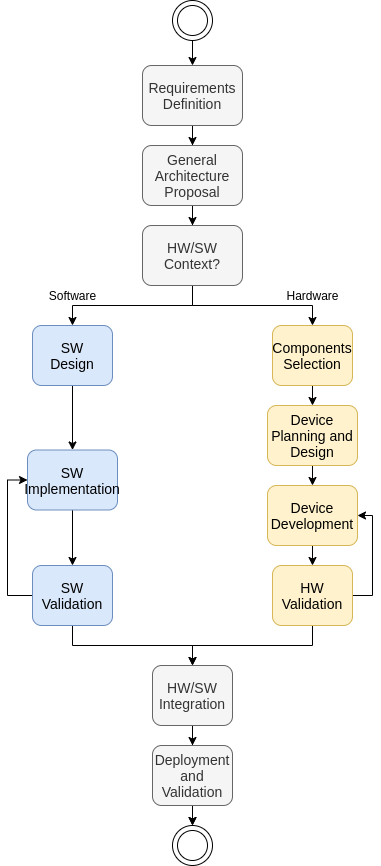
\includegraphics[width=.95\linewidth]{Figures/codesign-1.0.png}  
  \caption{Co-design considering HW/SW}
  \label{fig:codesign-1.0}
\end{subfigure}
\begin{subfigure}{.4\textwidth}
  \centering
  % include second image
  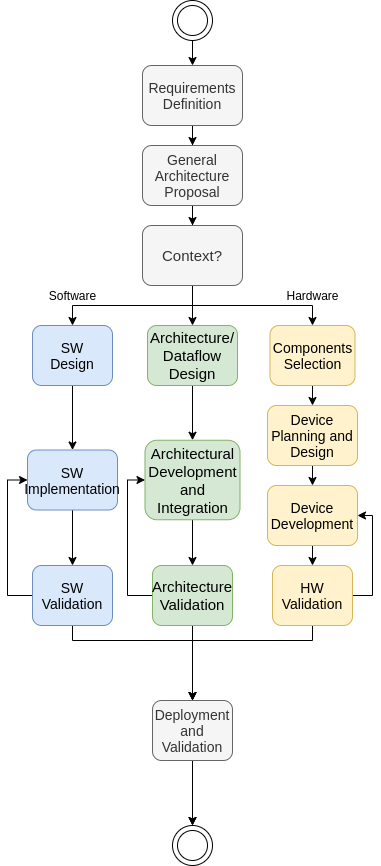
\includegraphics[width=\linewidth]{Figures/codesign-2.0.png}  
  \caption{New co-design approach}
  \label{fig:codesign-2.0}
\end{subfigure}
\caption{Co-design principle diagrams. The traditional approach does not consider architectural aspects in parallel with the HW and SW design.}
\label{fig:codesign-all}
\end{figure}

The traditional co-design approach typically begins with defining requirements and proposing a general architecture. Then, the constraints are segregated between hardware and software contexts, and the development of both aspects proceeds in parallel. After validating both components, the solution is integrated. This architecture is effective for designing single solutions for wearable and embedded systems, regardless of their abstraction levels. However, when dealing with multiple and variable architectures, this approach becomes fragile. If the validation after integration fails due to architectural traits, the solution becomes obsolete. This problem becomes even more critical when designing a Wearable Edge AI, where such factors cannot be ignored.

Thus, we suggest that architecture validation should be a new branch after context splitting. When designing new devices, identifying the essential aspects of architectural design and validating these designs during the proposal process is crucial. Finally, the integration must happen in parallel, and the last stage is deploying and validating all systems together. In the architecture branch, represented by green blocks in Figure \ref{fig:codesign-2.0}, there are three new stages:

\begin{itemize}
    \item \textit{Architecture/Dataflow Design}: In this stage, the proposal must identify how the devices communicate within the network. In the context of IoT and Edge Computing, devices communicate with each other providing services, insights, and information. Integrating devices in the same WBAN/WPAN, or even multiple devices with multiple WLAN users, requires a dataflow design.
    \item \textit{Architectural Development and Integration}: After defining the roles of each device within the network, as well as the integration protocols, the architecture must be developed in parallel with the integration of hardware components and individual software traits.
    \item \textit{Architecture Validation}: Like the other branches, the architecture must also be validated using formally-defined tests. This aspect enforces the design process and identifies flaws in the development process that must be assessed.
\end{itemize}

As displayed, these conditions help assessing the possibility of creating solutions combining the concepts of wearable computing, edge computing, and AI. We have previously studied the development of an Edge AI concept. Now, we define Wearable Edge AI as the set of methods that describes the design process and validation of solutions that combine wearable computing and Edge AI concepts in developing novel appliances, systems, and applications to solve real-world problems.

% \subsection{Hardware constraints}

% \subsection{Software constraints}

% \subsection{Architecture constraints}

\cleardoublepage
  \chapter{Case Study - Wearable Edge AI towards environmental studies}
\label{chap:ecology}

\nomenclature{VAE}{Variational Autoencoders}
\nomenclature{GAN}{Generative Adversarial Network}
\nomenclature{GRP}{Gaussian Random Process}
\nomenclature{GPE}{Gaussian Process Estimator}
\nomenclature{WLAN}{Wireless Local Area Network}
\nomenclature{MLP}{Multi-Layer Perceptron}
\nomenclature{LIDAR}{Light Detection and Ranging}
\nomenclature{IMU}{Inertial Measurement Unit}

This chapter is dedicated to the evaluation of the case-studies developed towards our first stakeholders. In the introductory section, we defined these target audience as the researchers, students, professors, and practitioners within ecology. We developed applications within three main branches: leaf damage estimation, diseases evaluation and mapping, and ants distribution and couting estimation.

\section{Leaf damage estimation}

The first application in our context is the leaf damage estimation. This information is important for the stakeholders related to the ecological field. For instance, researchers use this variable as an indicator to analyze the ecosystem interactions \cite{muiruri2019forest,benitez2018effect}, or even to analyze the impact of predators in crops \cite{saidov2018first,baudron2019understanding}.

\subsection{Requirements}

The first step in this analysis is evaluating the requirements for the proposed method. For this matter, we display a version of the co-design diagram presented in Figure \ref{fig:simplified-codesign-1}, which is a simplification of the diagram presented in Figure \ref{fig:codesign-2.0}. 

\begin{figure}[ht!]
    \centering
    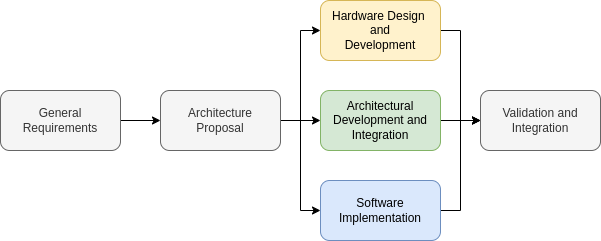
\includegraphics[width = .8\linewidth]{Figures/simplified-codesign.png}
    \caption{Simplified Co-design diagram.}
    \label{fig:simplified-codesign-1}
\end{figure}

This representation displays the need to raise the constraints for the application and classify them into the hardware, software or architectural domain. The constraints identified for this matter are:

\begin{itemize}
    \item The application must reconstruct the leaf shape using artificial intelligence [\textit{Software}].
    \item The application must have a mean to extract a single leaf image from the environment [\textit{Hardware}].
    \item The application must move the captured image into an AI accelerated hardware [\textit{Architecture}].
    \item The image from the leaf must be converted into a mask using image processing [\textit{Software}].
\end{itemize}

Given these constraints, we proposed the usage of a conditional GAN using the Tensorflow environment, allowing the integration with embedded AI accelerated hardware. We also propose the means in which a user can extract a leaf image which can input into such algorithm.

\subsection{Method overview}

\begin{figure}[ht!]
    \centering
    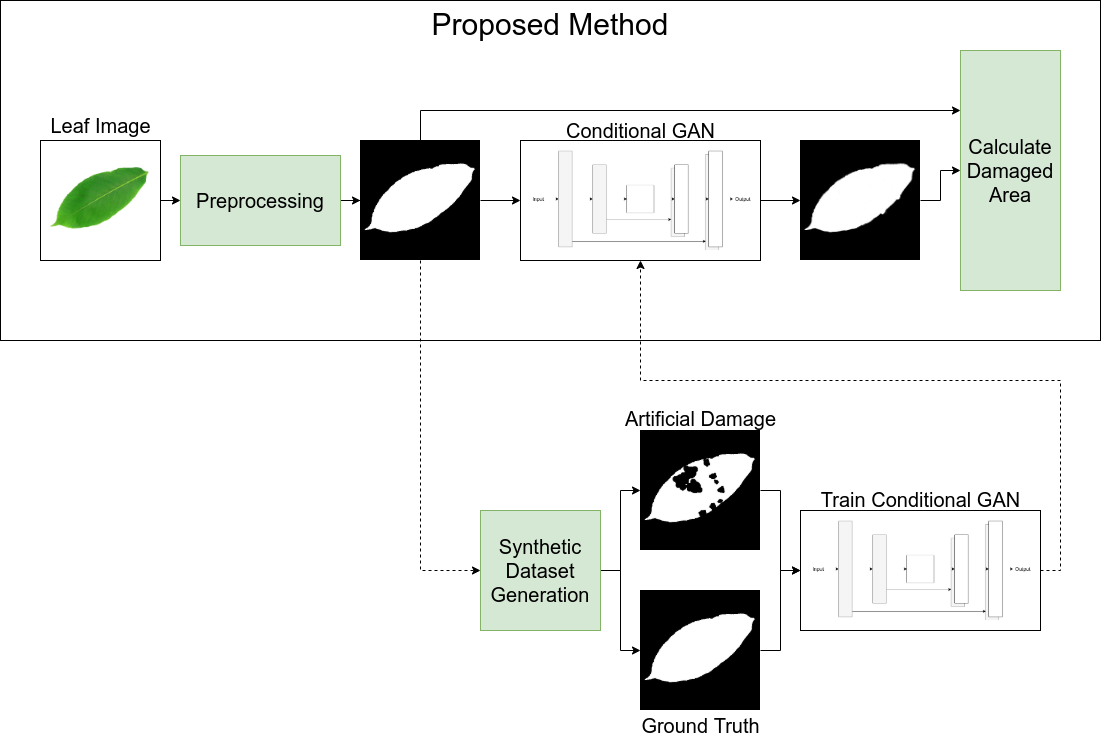
\includegraphics[width = .8\linewidth]{Figures/method-overview.png}
    \caption{Proposed Method and Work Overview}
    \label{fig:method-overview}
\end{figure}

The primary process of our proposed method begins with a preprocessing step that extracts a mask of the leaf area in the image, separating it from the background. The segmented image is then fed into a Conditional GAN model trained to produce an estimated original leaf shape. Lastly, we compare the output with the input image to determine the estimated percentage of defoliation. Figure \ref{fig:method-overview} provides a visual representation of this method.

In addition, we employed the preprocessing method to create a database of masks that includes the complete leaf shapes. These images were utilized to produce a synthetic database that includes leaf masks with artificially induced damage. The latter database was used to train the Conditional GAN method to obtain the test model, utilizing the original masks database as the ground truth. Figure \ref{fig:method-overview} also illustrates this series of stages.

%==========================================
\subsection{Datasets Description}

In this study, we worked with two distinct databases. The first one, referred to as FLAVIA henceforth, was introduced by Wu et al. \cite{wu2007leaf}. This dataset comprises 1907 colored images of leaves from 33 distinct plant species, with a resolution of 1600x1200 pixels. We utilized this dataset to create the synthetic database and for model training, validation, and testing purposes.

The second dataset we used is the Middle European Woods dataset presented by Novotny and Suk \cite{novotny2013leaf}. We will refer to this dataset as MEW 2012 in the rest of the paper. It consists of 9745 images of leaves from 153 different species, already binarized and available in various resolutions. We employed this dataset to conduct additional tests on the shape reconstruction and damage estimation process.

%==========================================
\subsection{Preprocessing}

As previously mentioned, the initial step in the data flow is preprocessing, which aims to extract the image from the background. We employed this technique to create a synthetic database that includes leaf masks with artificially induced damage. Additionally, we utilized the preprocessing method to generate a database of masks that includes the complete leaf shapes. The preprocessing stage comprises six consecutive steps:

\begin{enumerate}
    \item Convert to grayscale;
    \item Insert paddings to turn the image into a square shape;
    \item Reduce the size of the image to 400x400;
    \item Enhance the contrast using a radiometric transformation;
    \item Calculate the threshold using Otsu's method;
    \item Binarize the image;
\end{enumerate}

The initial step involves converting the image colorspace to grayscale. We then add padding to the image to shape it into a square. The padding is selected based on the highest pixel value to improve binarization performance when using thresholding algorithms. Following this, we employ a radiometric transformation to enhance the image contrast, as per Equation \ref{eq:radtransf}. In this equation, $G_i(x,y) \in [0,1],$ and $G_i(x,y) \in \mathbb{R}$ represent the normalized pixel values of the original image. It is worth noting that $G_f(x,y) \in [0,1],$ and $G_f(x,y) \in \mathbb{R}$ represent the output process parameters.

\begin{equation}
\label{eq:radtransf}
    G_f(x,y) = G_i(x,y)^{10}.
\end{equation}

Following the contrast enhancement stage, we move on to binarization. To achieve this, we utilized Otsu's method \cite{otsu1979threshold} to identify the separation threshold between the leaf and the background. This method works by minimizing the intra-class variance function, as defined in Equation \ref{eq:intraclass-variance}.

\begin{equation}
\label{eq:intraclass-variance}
    \sigma^2_b(k) = \frac{[\mu_T\omega(k)-\mu(k)]^{2}}{\omega(k)(1-\omega(k))}
\end{equation}

Where $k$ is the highest number of all the possible threshold values and:

\begin{align}
    \omega(k) = \sum_{i = 1}^{k}p(i);\\
    \mu(k) = \sum_{i = 1}^{k}i \dot p(i);\\
    \mu_T = \sum_{i = 1}^{L}i \dot p(i).
\end{align}

The values required for this method are obtained from the histogram, normalized as a probability density function represented by $p(i)$, for the $L$ candidate threshold values in the histogram. This approach provides a reliable estimation for the threshold value required to segment the image from its background. In this equation, $\omega(k)$ represents the class probability, $\mu(k)$ represents the class means, and $\mu_T$ represents the global mean. The variable $i$ represents all possible pixel values present in the histogram. Assuming every possible value of $k$ falls within the range of $[0,255]$ and is a natural number, all possible values of $i$ should be $i \in [1,255],$ $i \in \mathbb{N}$.

We also used this method to prepare the synthetic database, which was employed to train the conditional GAN method to obtain the test model using the original masks database as the ground truth. During the synthetic dataset generation, we removed internal holes to create ideal leaf images. Additionally, we developed a novel method for creating randomly artificial damaged leaf images, which we used to generate a dataset for training the conditional GAN.

%==========================================
\subsection{Synthetic Dataset Generation}

As previously mentioned, the preprocessing pipeline was utilized in the synthetic dataset generation process. We employed this method to prepare the images from the dataset for the application. In this section, we present the pipeline involved in producing images with synthetic damage and the processes included in this pipeline.

Most leaves in the dataset are undamaged, while some may show slight damage or light reflection spots. To better represent the ideal leaf shape, we selected the largest contour recognized after binarization to create a complete leaf representation. Using this technique, we generated 1907 masks corresponding to the 1907 images in the dataset. To create a supervised learning dataset in the next stage, we needed to introduce artificial measurable damage into the leaf masks.

In this stage, we discuss how we created artificial random damage on the leaves. Similar to Da Silva et al. \cite{da2019estimating}, we applied artificial damage techniques to generate a training dataset. We initially assumed that the leaf had a slightly higher probability of having damage at its borders. Therefore, we created a 2-D probability distribution, $g(x,y)$, centered on the $(x_0,y_0)$ average center position of the $x$ and $y$ coordinates of the binarized leaf mask image. Equation \ref{eq:gauss} represents this 2-dimensional Gaussian distribution centered at $(x_0,y_0)$, with a standard deviation of $\sigma$.

\begin{equation}
\label{eq:gauss}
    g(x,y) = e^{-\frac{(x-x_0)^2 + (y-y_0)^2}{2 \dot \sigma^2}}.
\end{equation}

Furthermore, we created a probability function $p(x,y)$, for the damage using $g(x,y)$ according to the following equation:

\begin{equation}
    {p}(x,y) = \frac{1-g(x,y)}{2} + P_0.
\end{equation}

In this scenario, $P_0$ represents the minimum probability offset. The probability of damage beyond the leaf's boundaries in the image must be zero. This condition is achieved by multiplying the probability function by the leaf mask. During the first stage of this study, we selected a baseline value of $P_0 = 0.3$ and $\sigma = 100$, based on practical tests conducted on the databases. In the second stage, we opted for a baseline value of $P_0 = 0.6$ and $\sigma = 10000$, to generate more damage on average. Figure \ref{fig:leaf_pdf} illustrates the probability function for one of the leaves in our dataset.

\begin{figure}[h!]
    \centering
    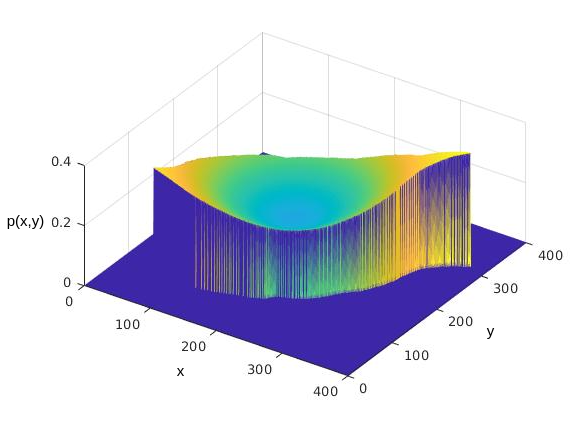
\includegraphics[width = .55\linewidth]{Figures/leaf_pdf.png}
    \caption{Example of damage probability density distribution. This function is used to generate the artificial damage.}
    \label{fig:leaf_pdf}
\end{figure}

\begin{figure}[h!]
    \centering
    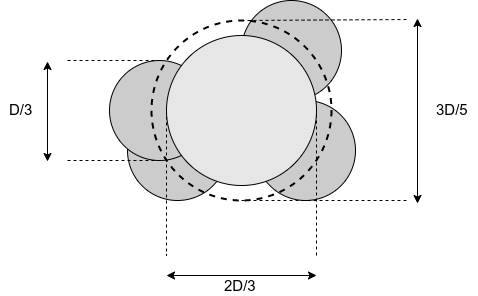
\includegraphics[width = .45\linewidth]{Figures/artificial-damage.png}
    \caption{Illustration of the punctual artificial damage generation method \cite{iceis21leaf}.}
    \label{fig:artificial-damage}
\end{figure}

The damage generated at a point follows a certain rule. Initially, we draw a circle with a diameter of $2D/3$ for a given reference size of $D$. Subsequently, we draw four circles with a diameter of $D/3$, centered at random points located over a virtual circle with a diameter of $3D/5$. Figure \ref{fig:artificial-damage} depicts the punctual artificial generation method.

The artificial damage generation algorithm selects several random coordinates and checks the function to determine whether it should insert damage at that point. If the answer is positive, it injects the loss at the spot by randomly selecting a reference size.

To create the synthetic dataset, we generated 12 versions of each leaf with random losses. We selected a pixel located at a coordinate $(x,y)$ as a candidate for receiving the artificial damage. Damage occurs only if the pixel is located within the leaf boundaries. For the first four images, we ran the method with 100 coordinates. For the fifth to eighth images, we executed the procedure with 200 coordinates. For the final four images, we performed the process with 300 coordinates. The resulting dataset consisted of 22884 shapes with varying levels of artificially generated damage.

%==========================================
\subsection{Conditional GAN Architecture}

Our implementation takes the work of Isola et al. \cite{isola2017image} as a baseline. For this matter, we applied a U-Net-based conditional GAN architecture. This network has two main modules: a generator and a discriminator. At first, the generator takes an input image and produces a predicted output. Then, the discriminator evaluates the prediction.

In this work, the main architecture is based on a U-Net. U-Nets are generative models of deep neural networks. Originally, this technique was proposed to perform segmentation in biomedical images \cite{ronneberger2015u}. They are similar to Variational Autoencoders (VAEs) \cite{hou2017deep}, and due to their generative capability, they can be used to reconstruct images pixel-by-pixel. These networks are applied for recognition and segmentation \cite{dong2017automatic,oktay2018attention} and for reconstruction \cite{hyun2018deep,antholzer2018photoacoustic}.

\subsubsection{Generator}

The generator's architecture is based on an Encoder-Decoder network. For this implementation, a U-Net was used, which has interconnected mirrored layers. The encoder consists of 8 layers (256x256, 128x128, 64x64, 32x32, 16x16, 8x8, 4x4, 2x2), with batch normalization in the intermediate layers. The output also has 8 layers (1x1, 2x2, 4x4, 8x8, 16x16, 32x32, 64x64, 128x128), with batch normalization in the intermediate layers.


\subsubsection{Discriminator}

On the other hand, the discriminator follows a PatchGAN architecture, which is similar to the encoding section of an encoder-decoder network. In this implementation, the discriminator consists of 5 layers (256x256, 128x128, 64x64, 32x32, 31x31), with batch normalization between the intermediate layers. 

\subsubsection{Training}

The network uses a two-part training method. Initially, the discriminator is trained based on the baseline answers. After that, the generator weights are updated based on the baseline truth and the discriminator guess. The training algorithm was performed for 20 epochs, with the first results being better than the ones presented in the literature. However, to avoid overfitting, the network was trained for an additional 5 epochs, which resulted in a significant improvement. As a result, the error becomes much smaller, making it state-of-the-art on the proposed problem.

%=========================================
\subsection{Damage Estimation}

In the previous section, we discussed the network architecture and its training process. In the preprocessing stage, the image is first converted to grayscale and then subjected to a binarization process. The resulting image is then used as input for the conditional GAN, which produces a mask that represents the predicted original shape. Finally, to calculate the damage percentage, we use the following formula:

\begin{equation}
	P_d = (1 - \frac{\sum_{i,j} Im_d(i,j)}{\sum_{i,j} Im(i,j)}) \times 100 (\%).
\end{equation}

Here, $P_d$ represents the damage percentage, $\sum_{i,j} Im_d(i,j)$ represents the sum of the binarized value (0 or 1) of each pixel of the damaged leaf image, and $\sum_{i,j} Im(i,j)$ represents the sum of the binarized value (0 or 1) of each pixel of the baseline image. We used the original image mask as the baseline for calculating the ground truth values of damage, while the model's outputs were used to calculate the predicted damage.

%==========================================
\subsection{Evaluation Methods}

In the previous section, we discussed the neural network used to estimate the original shape of damaged leaves, as well as the image datasets and artificial damage generation process used to create the synthetic dataset. In this section, we will focus on the methods used to evaluate the prediction quality.

We started with 22884 original images and used the first 22833 for our analysis. These images were randomly divided into three separate sets: 10\% for validation, 10\% for testing, and the remaining 80\% for training the algorithm. In the second stage, we repeated the process with modified parameters that allowed for more damage. We also used the 22884 images to create a dataset with the same proportions.

After training the model, we performed a round of predictions on the MEW 2012 dataset. To speed up the generation process, we reduced the images to 256x256 pixels and randomly applied 10 to 40 damage coordinates with a probability of $P_0 = 0.7$, resulting in a total of 38980 images. Although the generation process differed slightly, the images had to be resized to 400x400 pixels to be used with the model.

\subsubsection{Damage Estimation Evaluation}

Similar to Da Silva et al. \cite{da2019estimating}, we calculated the real defoliation percentage $d_r$ and the estimated defoliation percentage $d_e$. These values were measured on both the validation and test sets, as we generated the synthetic dataset from the ground truth. We evaluated the Root Mean Square Error (RMSE), which is calculated using the following equation:

\begin{equation}
	\label{eq:RMSE}
	RMSE = \sqrt{\frac{1}{n} \sum (d_e - d_r)^2}.
\end{equation}

Furthermore, we conducted a series of quantitative and qualitative analyses based on the prediction results.

\subsubsection{Shape Reconstruction Evaluation}

In the previous subsection, we discussed the evaluation method used for the damage estimation process. In addition to analyzing the quality of the defoliation estimation method, we also conducted a quantified evaluation of the image reconstruction process. To do this, we employed the dice coefficient, which is a widely used method for evaluating image similarity \cite{gencctav2012unsupervised,sampat2009complex,shamir2019continuous,mun2017comparison,nitsch2019automatic}. This measurement is used to compare areas and can be easily applied using binarized images. The dice coefficient ($DC$) is calculated for a pair of images ($A$ and $B$) using the following equation:

\begin{equation}
	\label{eq:dice}
	DC = \frac{2 \|(A \cap B)\|}{\|A\| +\|B\|}
\end{equation}

The resulting coefficient value is always in the range of [0, 1]. A high dice coefficient value indicates that the images are highly similar. Therefore, we used this factor to measure the success of the shape reconstruction process by calculating the dice coefficient to compare the ground truth and model output images.

%==========================================
\subsection{A Broader Evaluation on the Damage Estimation Results}

In the previous section, we discussed the method used to evaluate the leaf damage predictions, which involves estimating the original leaf shape using a Conditional GAN. In this section, we provide a broader overview of the original and predicted data to demonstrate the robustness of the proposed solution.

The first important set of results came from analyzing the RMSE values, which were defined by equation \ref{eq:RMSE}. The validation dataset had an RMSE value of 0.92 ($\pm$ 1.90), while the test dataset had a value of 0.92 ($\pm$ 1.85). As we previously mentioned, both the validation and test datasets had similar results for the RMSE value. After the second training stage, the error values were even lower. The validation dataset had an RMSE value of 0.61 ($\pm$ 0.99), and the test dataset had a value of 0.52 ($\pm$ 0.73). As previously shown, these results alone represent a significant improvement over the state-of-the-art. Table \ref{tab:RMSE} presents the results obtained.

\begin{table}[h!]
\caption{\label{tab:RMSE} RMSE Results}
\centering
\begin{tabular}{|l|l|l}
%\cline{2-3}
\hline
 & \multicolumn{1}{|c|}{Validation Set} & \multicolumn{1}{c|}{Test Set} \\ \hline
\multicolumn{1}{|c|}{Initial Round} & 0.92 ($\pm$ 1.90) \%& \multicolumn{1}{c|}{0.92 ($\pm$ 1.85) \%}\\ \hline
\multicolumn{1}{|c|}{Improved Round} & 0.61 ($\pm$ 0.99) \%& \multicolumn{1}{c|}{0.52 ($\pm$ 0.73) \%}\\ \hline
\end{tabular}
\end{table}


\begin{figure}[h!]
    \centering
    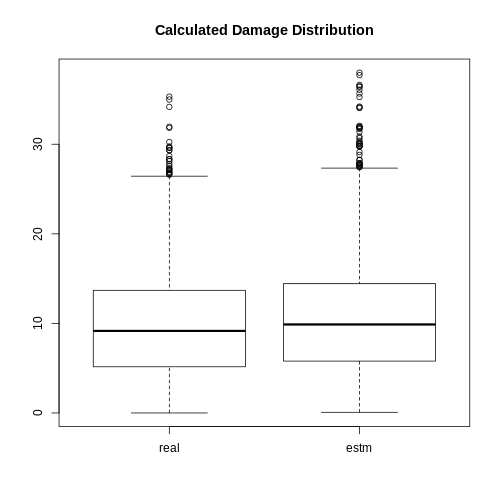
\includegraphics[width = .45\linewidth]{Figures/v1-val-dmgdst.png}
    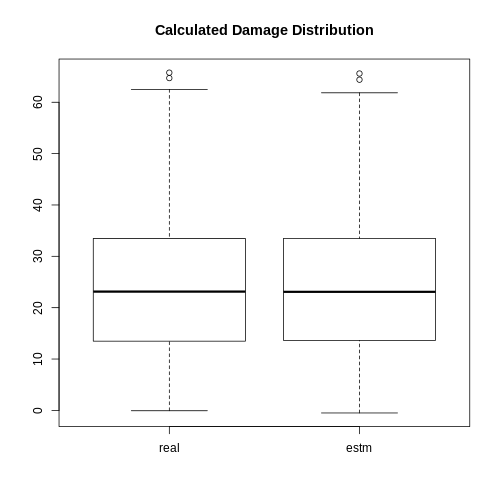
\includegraphics[width = .45\linewidth]{Figures/v2-val-dmgdst.png}
    \caption{Validation Set - Damage Distribution for the Initial and Improved Rounds. }
    \label{fig:validation_dist}
\end{figure}

For the initial stage, the validation set comprised 2283 randomly selected images from the original dataset. The estimated average damage on this set was 10.68 $\pm$ 6.34\%, with a maximum damage value of 37.99\%. The real average damage was 9.86 $\pm$ 6.03\%, with a maximum value of 35.31\%. In the second stage, the validation set contained 2288 randomly selected images from the original dataset. The estimated average damage on this set was 23.88 $\pm$ 12.97\%, with a maximum damage value of 65.59\%. The real average damage was 23.84 $\pm$ 13.06\%, with a maximum value of 65.76\%. The distribution plots for this data are shown in Figure \ref{fig:validation_dist}.

Additionally, we created a graph comparing the obtained data with the ground truth for both the initial and improved stages. Figure \ref{fig:validation_results} displays the results for the validation dataset in both rounds.

\begin{figure}[h!]
    \centering
    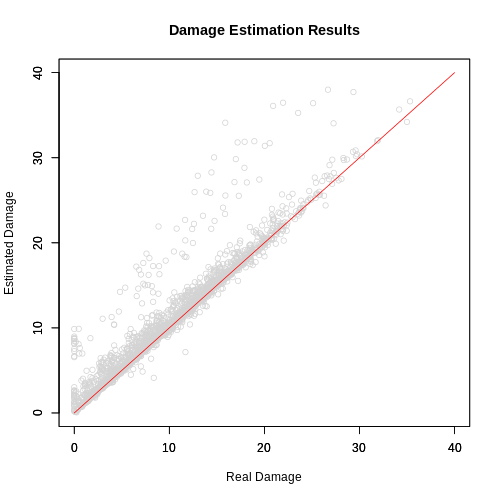
\includegraphics[width = .45\linewidth]{Figures/v1-val-estm.png}
    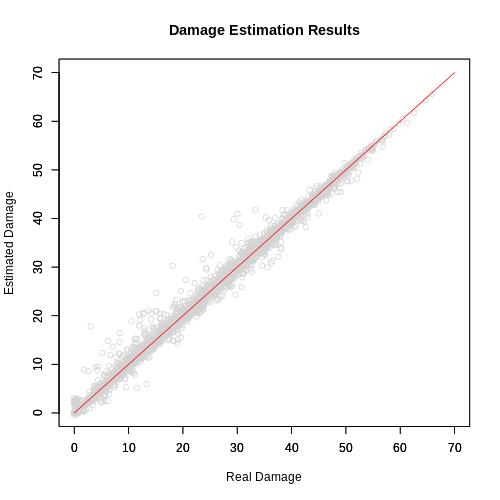
\includegraphics[width = .45\linewidth]{Figures/v2-val-estm.png}
    \caption{Validation damage estimation results for the Initial and Improved Rounds}
    \label{fig:validation_results}
\end{figure}

\begin{figure}[h!]
    \centering
    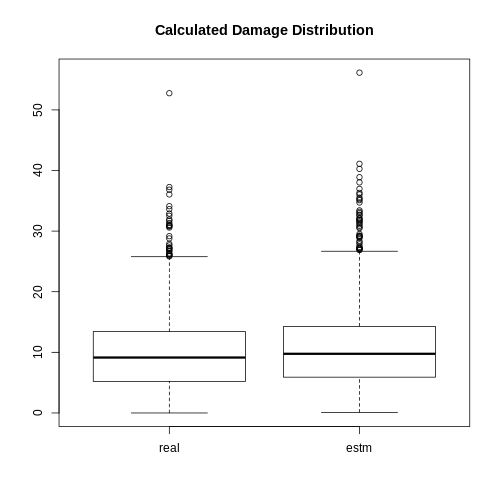
\includegraphics[width = .45\linewidth]{Figures/v1-tst-dmgdst.png}
    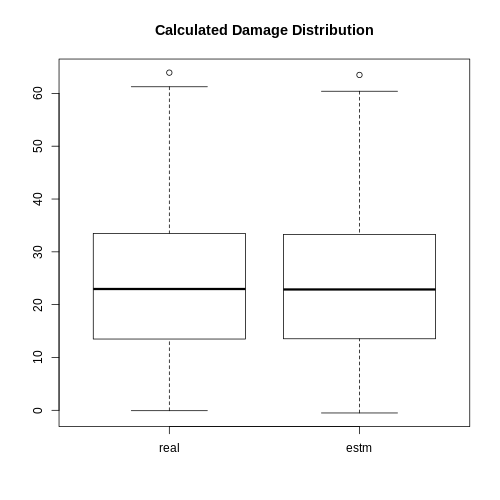
\includegraphics[width = .45\linewidth]{Figures/v2-tst-dmgdst.png}
    \caption{Test Set - Damage Distribution for the Initial Round}
    \label{fig:test_dist}
\end{figure}

Similarly, the test set comprised 2283 randomly selected images from the initial set. The average estimated damage in this set was 10.66 $\pm$ 6.44\%, with a maximum value of 56.14\%. The real damage distribution average and standard deviation were 9.84 $\pm$ 6.19\%, with a maximum damage of 52.74\%. In the second stage, the test set contained 2289 images. The average estimated damage in this set was 23.61 $\pm$ 12.99\%, with a maximum value of 63.49\%. The real damage distribution average and standard deviation were 23.68 $\pm$ 12.99\%, with a maximum damage of 63.92\%. The boxplots with the distribution of this data are shown in Figure \ref{fig:test_dist}.


\begin{figure}[h!]
    \centering
    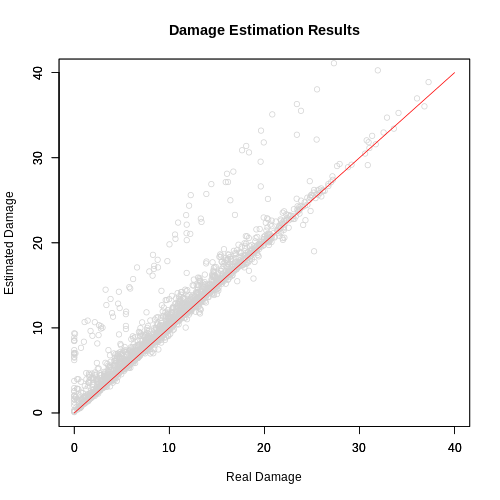
\includegraphics[width = .45\linewidth]{Figures/v1-tst-estm.png}
    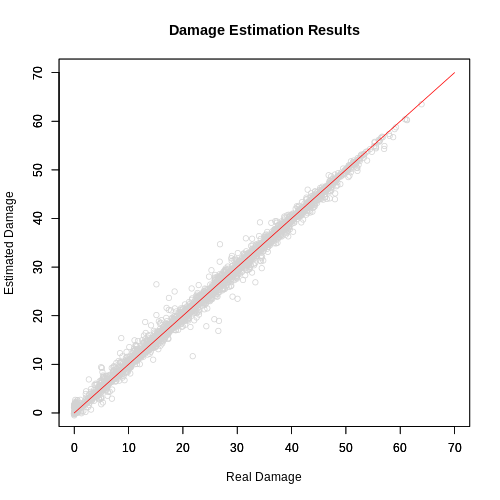
\includegraphics[width = .45\linewidth]{Figures/v2-tst-estm.png}
    \caption{Test set damage estimation results for the Initial Round}
    \label{fig:test_results}
\end{figure}

We also created a graph comparing the obtained data with the ground truth for the test dataset in both the initial and improved stages. Figure \ref{fig:test_results} displays the results. A qualitative analysis of the results indicates that the distributions of the sets are similar, which reinforces the RMSE parameter results.

\subsubsection{MEW 2012 Results}

As previously mentioned, we also conducted predictions on another database containing different species from the ones used during training. We selected MEW 2012, which comprised 9745 images, and generated 38980 images with artificial random damage for this purpose. 

\begin{figure}[h!]
    \centering
    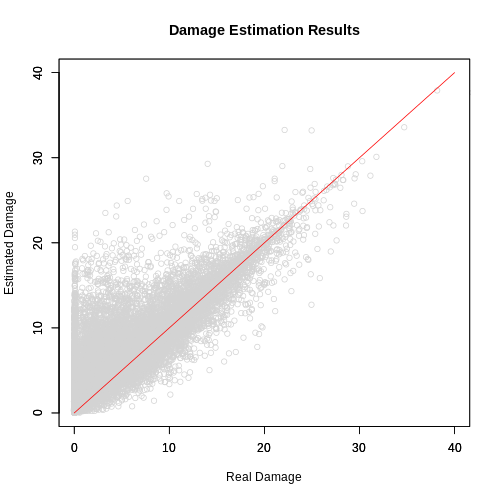
\includegraphics[width = .45\linewidth]{Figures/v1-mew2012-estm.png}
    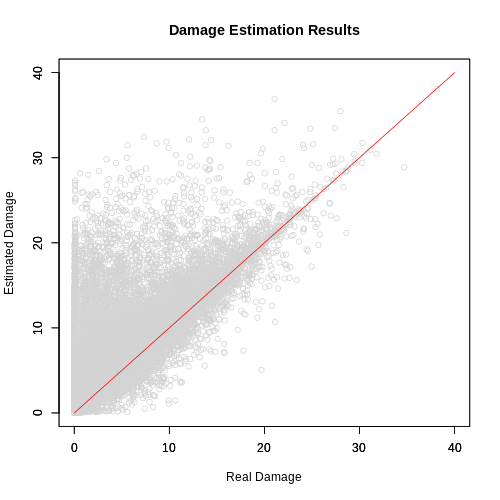
\includegraphics[width = .45\linewidth]{Figures/v2-mew2012-estm.png}
    \caption{MEW 2012 set damage estimation results for the Initial and Improved rounds}
    \label{fig:mew2012_results}
\end{figure}

The average estimated damage in MEW 2012 set is 5.05\%, with a standard deviation of 4.43\% and a maximum damage value of 37.90\%. The real damage distribution average and standard deviation were 3.93 $\pm$ 4.39\%, with a maximum value of 41.87\%. The RMSE for this prediction was 1.76 ($\pm$ 3.02).

We also presented a graph comparing the obtained data with the ground truth. Figure \ref{fig:mew2012_results} displays the results for the MEW 2012 dataset. As this dataset contained more species and samples, the distribution of predictions appeared wider during qualitative analysis. However, the RMSE result confirms that the prediction quality was similar, even with a dataset containing leaves from untrained species.


\subsubsection{Shape Reconstruction results}

To evaluate the shape reconstruction quality, we compared the network model's output with the ground truth initially generated or obtained from the datasets. We began by evaluating the distributions of the validation and test datasets and conducted a statistical analysis to determine if the predicted and original shapes represented different populations based on their dice coefficient results distribution. The population distributions are presented in Figures \ref{fig:val-dice-dist}, \ref{fig:val-dice-dist-2}, \ref{fig:tst-dice-dist}, \ref{fig:tst-dice-dist-2}, and \ref{fig:mew2012-dice-dist}.

\begin{figure}[h!]
    \centering
    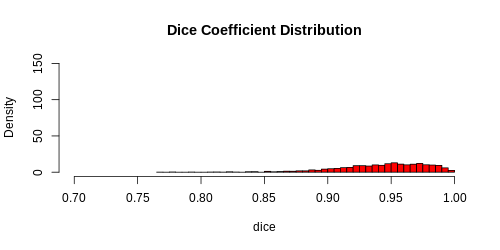
\includegraphics[width=.65\linewidth]{Figures/v1-val-dicedst-d.png}
    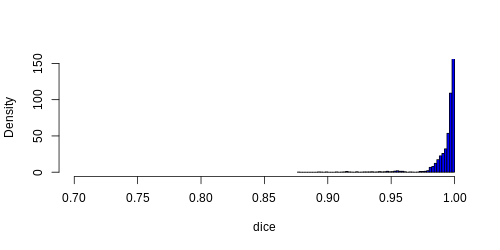
\includegraphics[width=.65\linewidth]{Figures/v1-val-dicedst-r.png}
    \caption{Dice coefficient distribution for the validation set - Initial Round}
    \label{fig:val-dice-dist}
\end{figure}

\begin{figure}[h!]
    \centering
    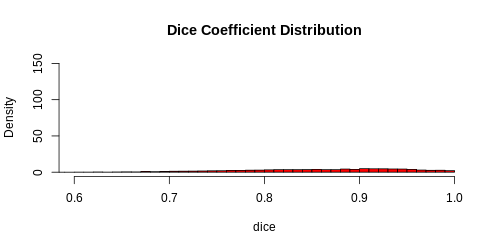
\includegraphics[width=.65\linewidth]{Figures/v2-val-dicedst-d.png}
    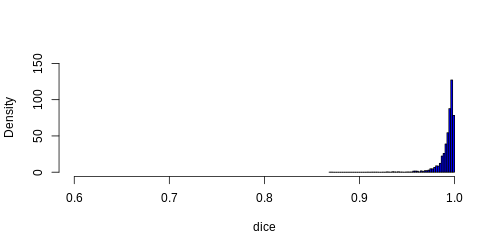
\includegraphics[width=.65\linewidth]{Figures/v2-val-dicedst-r.png}
    \caption{Dice coefficient distribution for the validation set - Improved Round}
    \label{fig:val-dice-dist-2}
\end{figure}

\begin{figure}[h!]
    \centering
    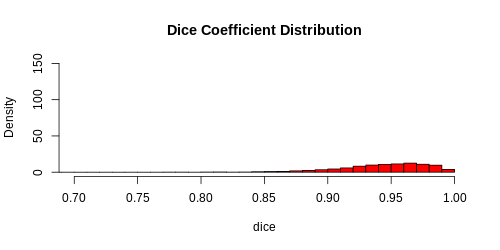
\includegraphics[width=.65\linewidth]{Figures/v1-tst-dicedst-d.png}
    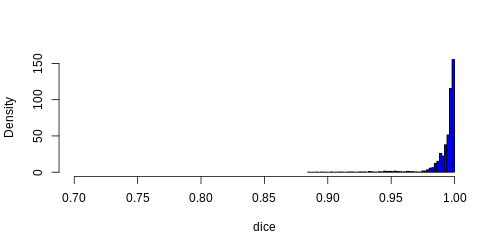
\includegraphics[width=.65\linewidth]{Figures/v1-tst-dicedst-r.png}
    \caption{Dice coefficient distribution for the test set - Initial Round}
    \label{fig:tst-dice-dist}
\end{figure}

\begin{figure}[h!]
    \centering
    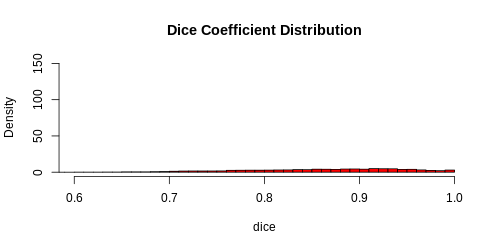
\includegraphics[width=.65\linewidth]{Figures/v2-tst-dicedst-d.png}
    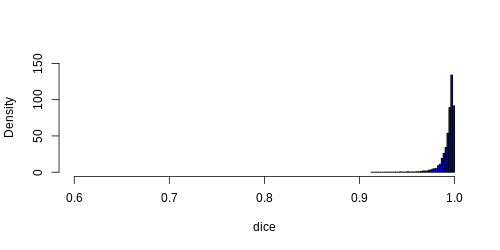
\includegraphics[width=.65\linewidth]{Figures/v2-tst-dicedst-r.png}
    \caption{Dice coefficient distribution for the test set - Improved Round}
    \label{fig:tst-dice-dist-2}
\end{figure}

\begin{figure}[h!]
    \centering
    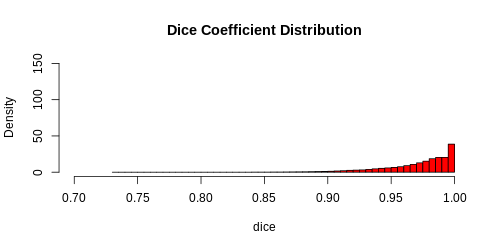
\includegraphics[width=.65\linewidth]{Figures/v2-mew2012-dicedst-d.png}
    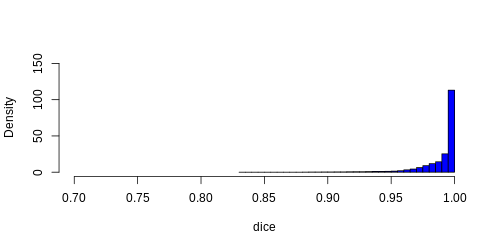
\includegraphics[width=.65\linewidth]{Figures/v2-mew2012-dicedst-r.png}
    \caption{Dice coefficient distribution for the MEW 2012 set}
    \label{fig:mew2012-dice-dist}
\end{figure}

In red, we plotted the dice coefficient comparing the damaged leaves with the original shapes, while in blue, we plotted the dice coefficient comparing the reconstructed leaves with the original shapes. The variances between the red and blue populations were different. Therefore, we chose to apply Welch's \textit{t}-test to compare the populations \cite{salkind2010encyclopedia}. For all studied cases, the \textit{p}-value was lower than $2.2 \times 10^{-16}$, indicating that the population means were not equal. In other words, the reconstruction process produced different shapes that were not caused by random events.

Regarding the reconstructed data, the average dice coefficient value for the validation set was 0.992 $\pm$ 0.008, while that for the test set was 0.993 $\pm$ 0.007. The worst-case values were 0.869 for the validation set and 0.912 for the test set. Finally, the average obtained from the MEW 2012 set was 0.988 $\pm$ 0.017.

\subsection{Technical Evaluation: How to embed this solution?}

In red, we plotted the dice coefficient comparing the damaged leaves with the original shapes, while in blue, we plotted the dice coefficient comparing the reconstructed leaves with the original shapes. The variances between the red and blue populations were different. Therefore, we chose to apply Welch's \textit{t}-test to compare the populations \cite{salkind2010encyclopedia}. For all studied cases, the \textit{p}-value was lower than $2.2 \times 10^{-16}$, indicating that the population means were not equal. In other words, the reconstruction process produced different shapes that were not caused by random events.

Regarding the reconstructed data, the average dice coefficient value for the validation set was 0.992 $\pm$ 0.008, while that for the test set was 0.993 $\pm$ 0.007. The worst-case values were 0.869 for the validation set and 0.912 for the test set. Finally, the average obtained from the MEW 2012 set was 0.988 $\pm$ 0.017.

\begin{enumerate}
    \item Interest region identification;
    \item Interest region segmentation;
    \item Image binarization.
\end{enumerate}

\begin{figure}[h!]
    \centering
    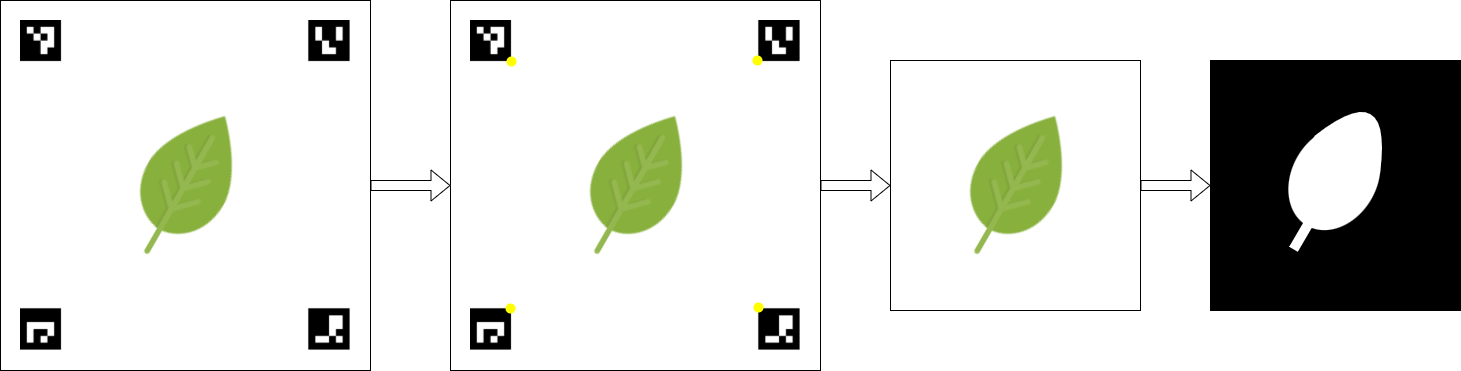
\includegraphics[width = \linewidth]{Figures/full-pipeline.png}
    \caption{Complete segmentation pipeline proposal}
    \label{fig:pipeline-proposal}
\end{figure}

The proposed pipeline is presented in Figure \ref{fig:pipeline-proposal}. The initial step in this process involves identifying the area where the user intends to place the leaf. This step is aided by the use of readily identifiable elements in the image, such as ArUco tags \cite{garrido2014automatic}. These tags are easily integrated into popular Computer Vision libraries and enable the identification of specific points. 

\begin{figure}[h!]
    \centering
    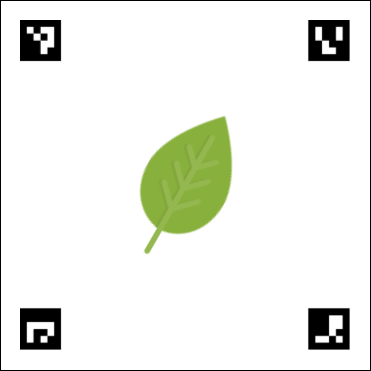
\includegraphics[width = .4\linewidth]{Figures/illustration.png}
    \caption{Illustration of the usage of ArUco tags to segment a map area.}
    \label{fig:illustration}
\end{figure}

We propose the use of four tags that delimit a square to aid in this process. The leaf should be positioned at the center of this square. This method helps to correct perspective issues that may arise due to camera tilt. An illustration of the proposed solution is presented in Figure \ref{fig:illustration}.

To segment the region, the algorithm must identify the four tags and extract the desired coordinates from each of them. Then, a perspective transformation is performed to convert the plane into a square. The expected results after this stage are displayed in Figure \ref{fig:stage-2}.

\begin{figure}[h!]
    \centering
    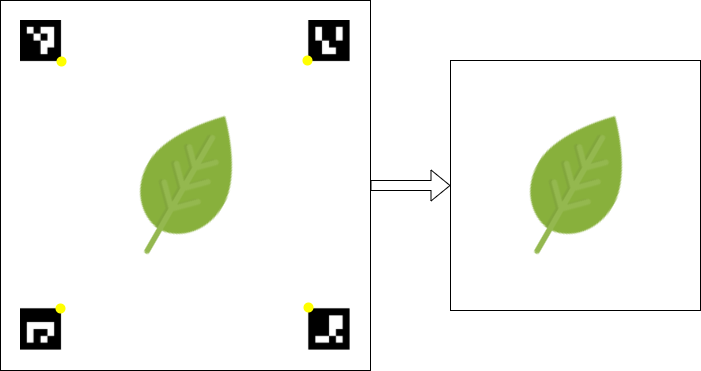
\includegraphics[width = .5\linewidth]{Figures/stage-2.png}
    \caption{Region segmentation process illustration}
    \label{fig:stage-2}
\end{figure}

After this stage, the algorithm obtains a square region with the leaf positioned above the background. At this point, we directly apply Otsu's binarization algorithm to the obtained segment. The expected result is displayed in Figure \ref{fig:stage-3}.

\begin{figure}[h!]
    \centering
    
\includegraphics[width = .5\linewidth]{Figures/stage-3.png}
    \caption{Binarization process illustration}
    \label{fig:stage-3}
\end{figure}

We tested this pipeline under two different conditions. The first condition was a bench test. We produced the background according to the planned and provided a mockup leaf to test the segmentation process. Then, we also performed a small field test, in which we tried to capture and segment a leaf in the field using a camera and submitting it to this same process. Figure \ref{fig:experiments-final} displays the results for both tests. Our experiments displayed overall satisfactory results in both the bench and the field tests. The algorithm was able to segment the leaf from the background properly.

\begin{figure}[h!]
    \centering
    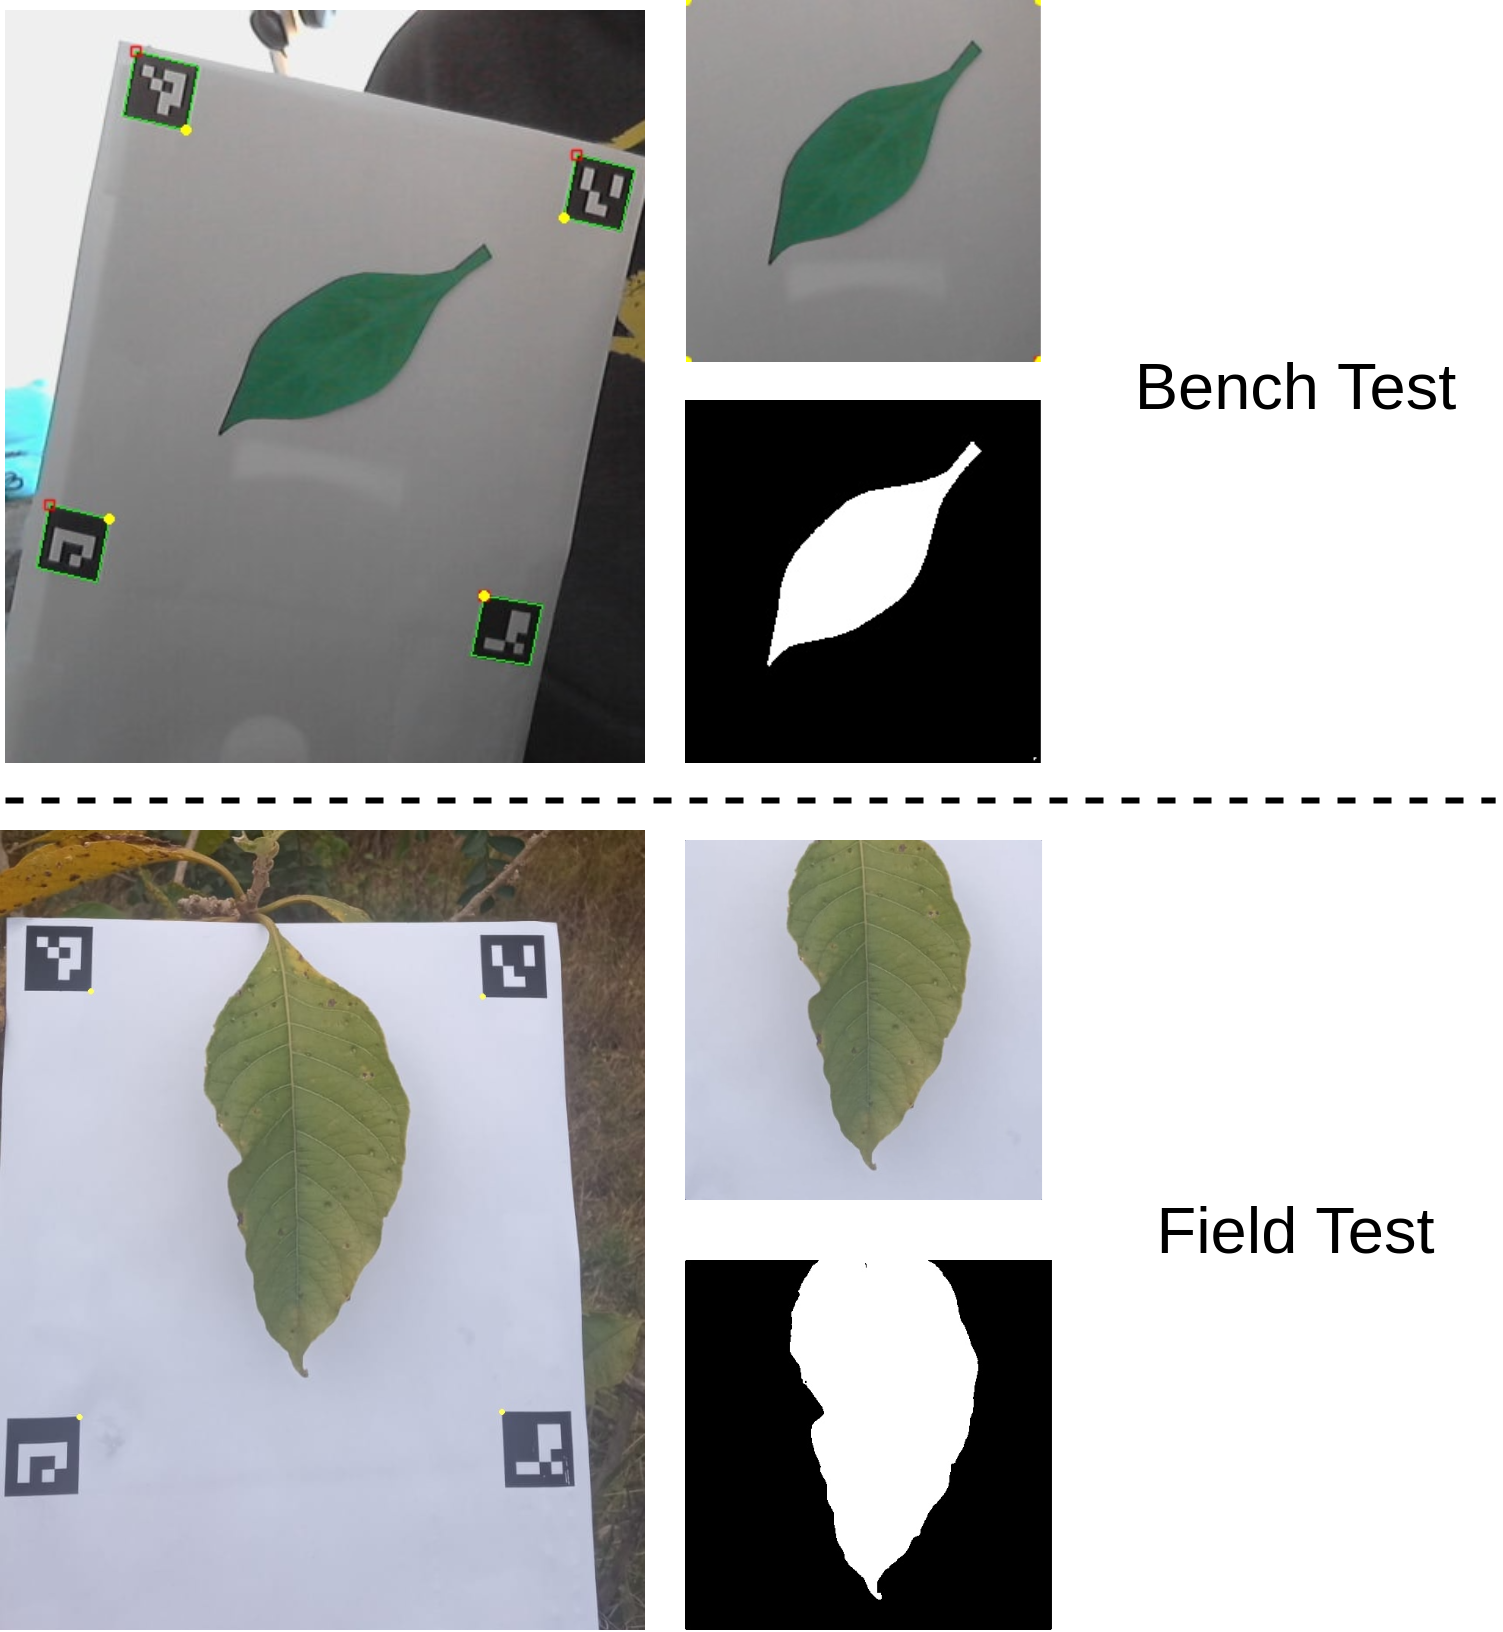
\includegraphics[width = .6\linewidth]{Figures/experiments.png}
    \caption{Experiments displaying the results of the proposed process. These experiments validate the usage of this technique to provide a mean to take this appliance onto the field.}
    \label{fig:experiments-final}
\end{figure}

%==========================================

\section{Evaluating and mapping diseases in forest canopies}

The case study involves a triangulation approach, where three individual climbers conducted a cylinder-transect investigation. This method is akin to the recommendation made by Ribeiro, Basset, and Kitching  \cite{ribeiro2014density} about density estimation. We employed this approach to develop the Edge AI system for identifying leaf diseases. The researchers initiate their approach by commencing at the highest point of the canopy and progressively descend downwards. They collect leaf samples along horizontal transects that are spaced at predetermined intervals until they reach the last stop. In this initial approach, to facilitate the division of data, we employ a backdrop template for sampling. The final destination is typically situated approximately 3 meters above ground level. The proposed methodology is depicted in Figure \ref{fig:cylinder}.

\begin{figure}[h]
    \centering
    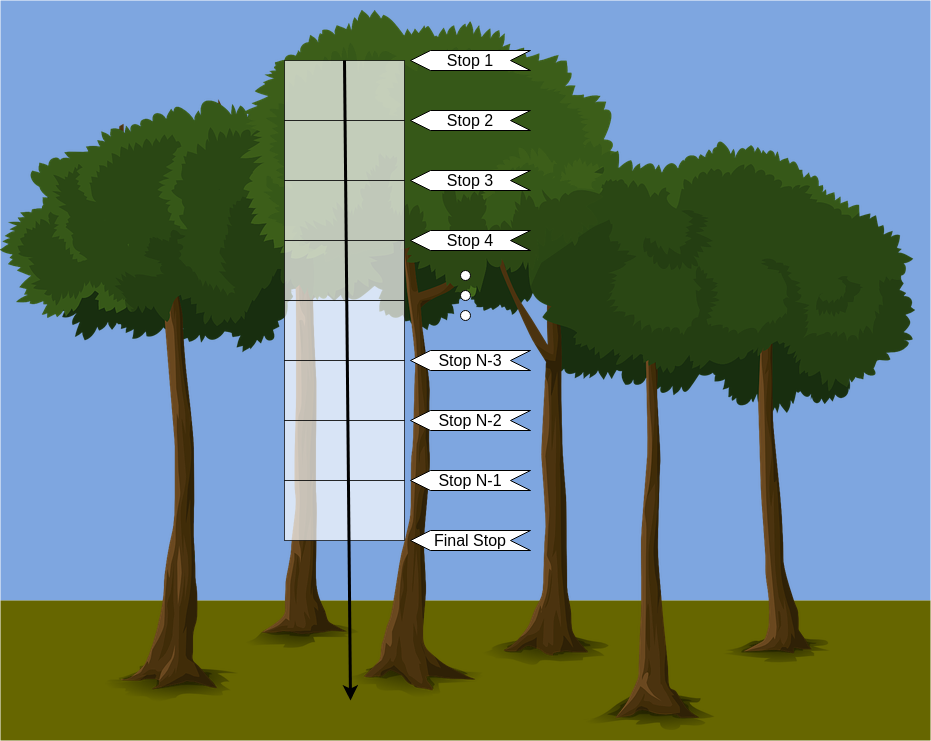
\includegraphics[width = .8\linewidth]{Figures/pin-cylinder.png}
    \caption{Illustration of the Cylinder-Transect study.}
    \label{fig:cylinder}
\end{figure}

Leaf conditions are highly significant markers of ecosystem health, as previously mentioned. García-Guzman et al. \cite{garcia2004incidence} demonstrated that in Mexican wet forests, the prevalence of diseased leaves can reach 65\% in highly infected areas, while it is only 2\% in locations with low infection rates. Given this baseline, we anticipate that the disease will be dispersed in both high and low infection locations whenever a pathogen is present in a canopy. From this viewpoint, we simulate the transmission of disease by utilizing a probability density function (PDF) that is centered on the location with the largest percentage of infected individuals. Figure \ref{fig:canopy-disease-spread} depicts a visual representation of a density gradient determined by a centered maximum.

\begin{figure}[h]
    \centering
    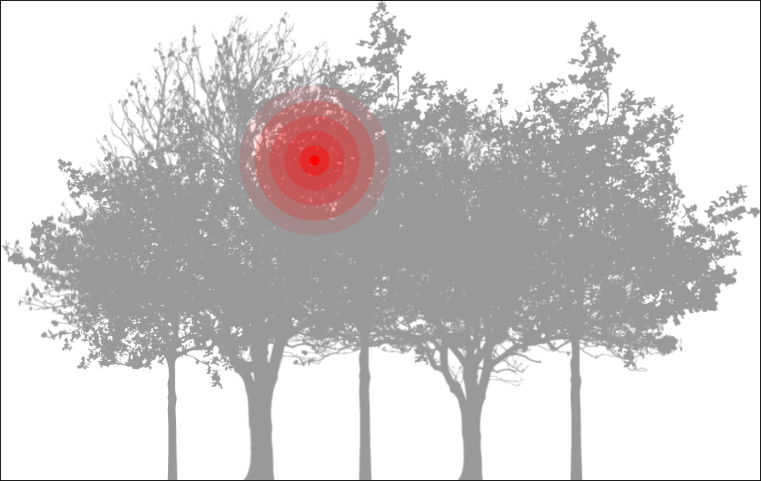
\includegraphics[width = .8\linewidth]{Figures/diseased-canopy.png}
    \caption{\color{black}Example of a possible location for a disease spread. We model this spread using a spatially-distributed probability density function (PDF).}
    \label{fig:canopy-disease-spread}
\end{figure}

We assume that the distribution is Gaussian in shape, extending across the canopy. Therefore, the distribution can be represented by a probability density function that follows a geometric function based on the Gaussian distribution. The function is expressed in Equation \ref{eq:pdf}. The function has the benefit of being able to represent the spread of the disease with only five parameters. The variable $p_0$ denotes the highest occurrence rate of the disease. The $\sigma$ parameter, as always, reflects the standard deviation. To simplify the analysis, we employed a uniform standard deviation across all three spatial dimensions. The $(x_0, y_0, z_0)$ coordinates represent the central point of the distribution. The objective of this work is not to delve into the intricacies of the modeling process, but rather to present a case-study that is straightforward and can be easily replicated.

\begin{equation}
\label{eq:pdf}
    P(x,y,z) = p_0 . e^{-\frac{(x-x_0)^2 + (y-y_0)^2 + (z-z_0)^2 }{2\sigma}}
\end{equation}

Several authors with prior experience in similar methodologies endorse the use of Gaussian-based models for disease transmission modeling. Soubeyrand, Enjalbert, and Sache \cite{soubeyrand2008accounting}  employed Gaussian-based modeling to simulate the circular diffusion of airborne plant disease. Pokharel and Deardon \cite{pokharel2016gaussian} conducted mathematical modeling of the transmission of infectious diseases using Gaussian distributions. In the midst of the COVID-19 pandemic, Ketu and Mishra \cite{ketu2021enhanced} utilized Gaussian-based models to forecast the spread of the disease.

Despite the existence of similar methods in the literature, we have selected this modeling approach over Gaussian random processes (GRPs) or Gaussian process estimators (GPEs) due to its distinct essential features, as highlighted by some of the writers. The authors Soubeyrand, Enjalbert, and Sache utilized GRPs in their suggested model, as outlined in their publication \cite{soubeyrand2008accounting}. The model involved the application of circular functions in a two-dimensional space to generate a preliminary representation. Our goal in this work is not to go into illness modeling. Therefore, we have chosen to develop a simplified model that relies on a single spatial function. Pokharel and Deardon \cite{pokharel2016gaussian} suggest employing Gaussian process approximations to construct emulators (GPEs) for a two-dimensional dynamic disease spread model. The objective differs in that the authors aim to incorporate additional variables and processes that are not the focus of this study.

Researchers employing the cylinder-transect approach in the canopy acquire the spatial arrangement of damaged and healthy leaves using established coordinates. While the depiction may appear uncomplicated, the process of doing a regression from density points in three-dimensional space to a continuous-space function is not straightforward. Therefore, we suggest employing a heuristic approach to acquire the parameters that more accurately depict the original function.

\subsection{Requirements}

To begin this study, it is necessary to assess the prerequisites for the proposed approach. To address this issue, we provide a modified version of the co-design diagram shown in Figure \ref{fig:simplified-codesign-2}, which is a simplified rendition of the diagram depicted in Figure \ref{fig:codesign-2.0}. 

\begin{figure}[ht!]
    \centering
    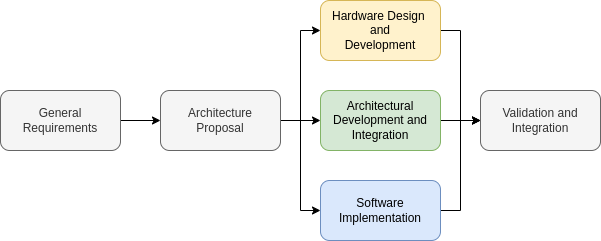
\includegraphics[width = .8\linewidth]{Figures/simplified-codesign.png}
    \caption{Simplified Co-design diagram.}
    \label{fig:simplified-codesign-2}
\end{figure}

This representation displays the need to raise the constraints for the application and classify them into the hardware, software or architectural domain. The constraints identified for this matter are:

\begin{itemize}
    \item As this system needs to be taken into the field, it needs to work for hours without a battery recharge or replacement. [\textit{Hardware}].
    \item It needs to be robust enough to take hits from branches and falling seeds or nuts. [\textit{Hardware}].
    \item As we propose a distributed system in a WBAN-Environment, both systems need to communicate with an application, working as web server nodes [\textit{Architecture}].
    \item The communication needs to be efficient to stream the data through this local network [\textit{Architecture}].
    \item The integrated architecture must present a mean to classify the leaves into diseased or healthy [\textit{Software}].
\end{itemize}

In this case, we proposed a cooperative wearable system in which several users can input gathered data into a local wireless server which provides the AI using its hardware acceleration. This system is able to run both a traditional machine learning method and a convolutional neural network, according to the available resources.

\subsection{General Architecture Proposal}

The suggested method utilizes a wearable distributed system that operates in both Wireless Body-Area Network (WBAN) and Wireless Local Area Networks (WLAN). This system is designed to enable the extraction of information using techniques such as Data Fusion, Image Processing, and Computer Vision. The provided diagram, labeled as Figure \ref{fig:architecture}, illustrates the suggested design for this system.

\begin{figure}[h!]
\centering
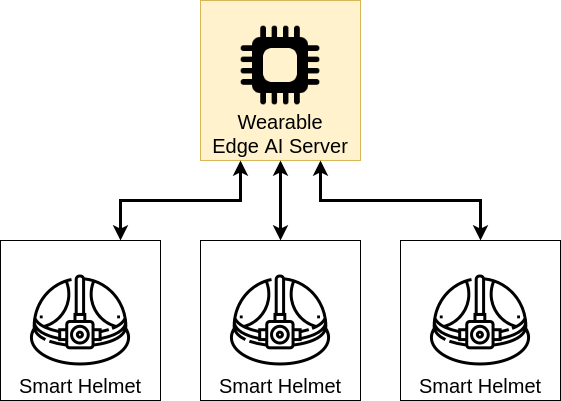
\includegraphics[width = .6\linewidth]{Figures/dataflow-2.png}
\caption{\label{fig:architecture}Proposed General Architecture. The smart helmets use the wearable Edge AI server to provide machine learning inferences.}
\end{figure}

The initial component of this system is the tangible nucleus. Since we are suggesting a wearable system, it is crucial that it is inconspicuous and does not cause any interference or disturbance \cite{bonato2003wearable}. Consequently, we constructed the system using hands-free technology for the user. The helmet is the optimal choice for meeting the wearable and research needs in terms of its physical core. The paper by Silva et al. \cite{silva2019toward} addressed the limitations imposed by certain appliances. Our main focus was to calculate the energy needs and usage for this particular system.

The subsequent component pertains to the fabrication of the sensor nodes that are based on the Internet of Things (IoT) technology. Every node is a Computer-on-Chip that has the ability to read sensor data, either single or numerous, process the data beforehand, and transmit it via either WBAN or WLAN. The selected sensors for enhancing environmental perception include a laser radar (LIDAR), a 9-Degree-of-Freedom Inertial Measurement Unit (9DoF IMU), and a conventional camera.

The Computer-on-Chip must possess the capability to access the necessary input/output ports from every sensor. Additionally, it is imperative that it possesses the capability to establish a wireless connection within the immediate vicinity of the body. Given the energy limitations of wearable systems, it is imperative that the Computer-on-Chip incorporates a processor with low power consumption. Therefore, ARM-based computer-on-chips are suitable solutions for this purpose. 

Typically, the preferred devices to serve as primary applications for this system are ARM-based Computer-on-Chips. These devices should include various I/O ports to connect the necessary sensors, as well as a network card that can transmit the data via a local wireless connection.

We choose the Wi-Fi network standard (IEEE 802.11) as the interface for our WLAN/WBAN. The decision was made considering the simplicity of developing web server solutions, the speed at which data can be transmitted, and the coverage area for WBAN/WLAN. Furthermore, it relied on the wider bandwidth capacity to ensure the quality of the connection, particularly while handling camera streaming. 

Each sensor node functions as a local webserver within this network. The application should explicitly request the sensor data from each node through the WBAN/WLAN. The application executes a data fusion technique. augments reality.

\subsubsection{Hardware Specification}

From the proposal, there are two main hardware element decisions: the \textit{Smart Helmet Hardware} and the \textit{Edge AI Node Hardware}.  In order to develop the intelligent helmet, we required a flexible and verified solution that includes a built-in camera. Conversely, the stage of selecting Edge AI Node Hardware must effectively balance performance and portability.

\paragraph{Smart Helmet Hardware}

This project is a progressive development of a wearable gadget designed for the purpose of studying and monitoring the ecological environment. Additional publications were authored by members of the research group, featuring findings that were previously examined. The articles \cite{silva2019toward, silva2019desenvolvimento} provide a detailed description of the hardware specification and its evaluation. The reproduction of the previously described evaluation is not the topic of this effort. Our objective is to include the suggested hardware into the Edge-AI architecture within this context.

This section offers a concise overview of the constructed wearable device and presents the necessary details and principles for the suggested integration. The hardware that has been created is a helmet consisting of sensors and a data processing unit. This tool was specifically designed for researchers and professionals who utilize the climb tree approach to gather data on natural habitats. 

\begin{figure}[ht]
\centering
\begin{subfigure}{.45\textwidth}
  \centering
  % include first image
  \includegraphics[width=\linewidth]{Figures/helmet2.JPG}  
  \caption{Assembled Wearable Device}
  \label{fig:proto}
\end{subfigure}
\begin{subfigure}{.45\textwidth}
  \centering
  % include second image
  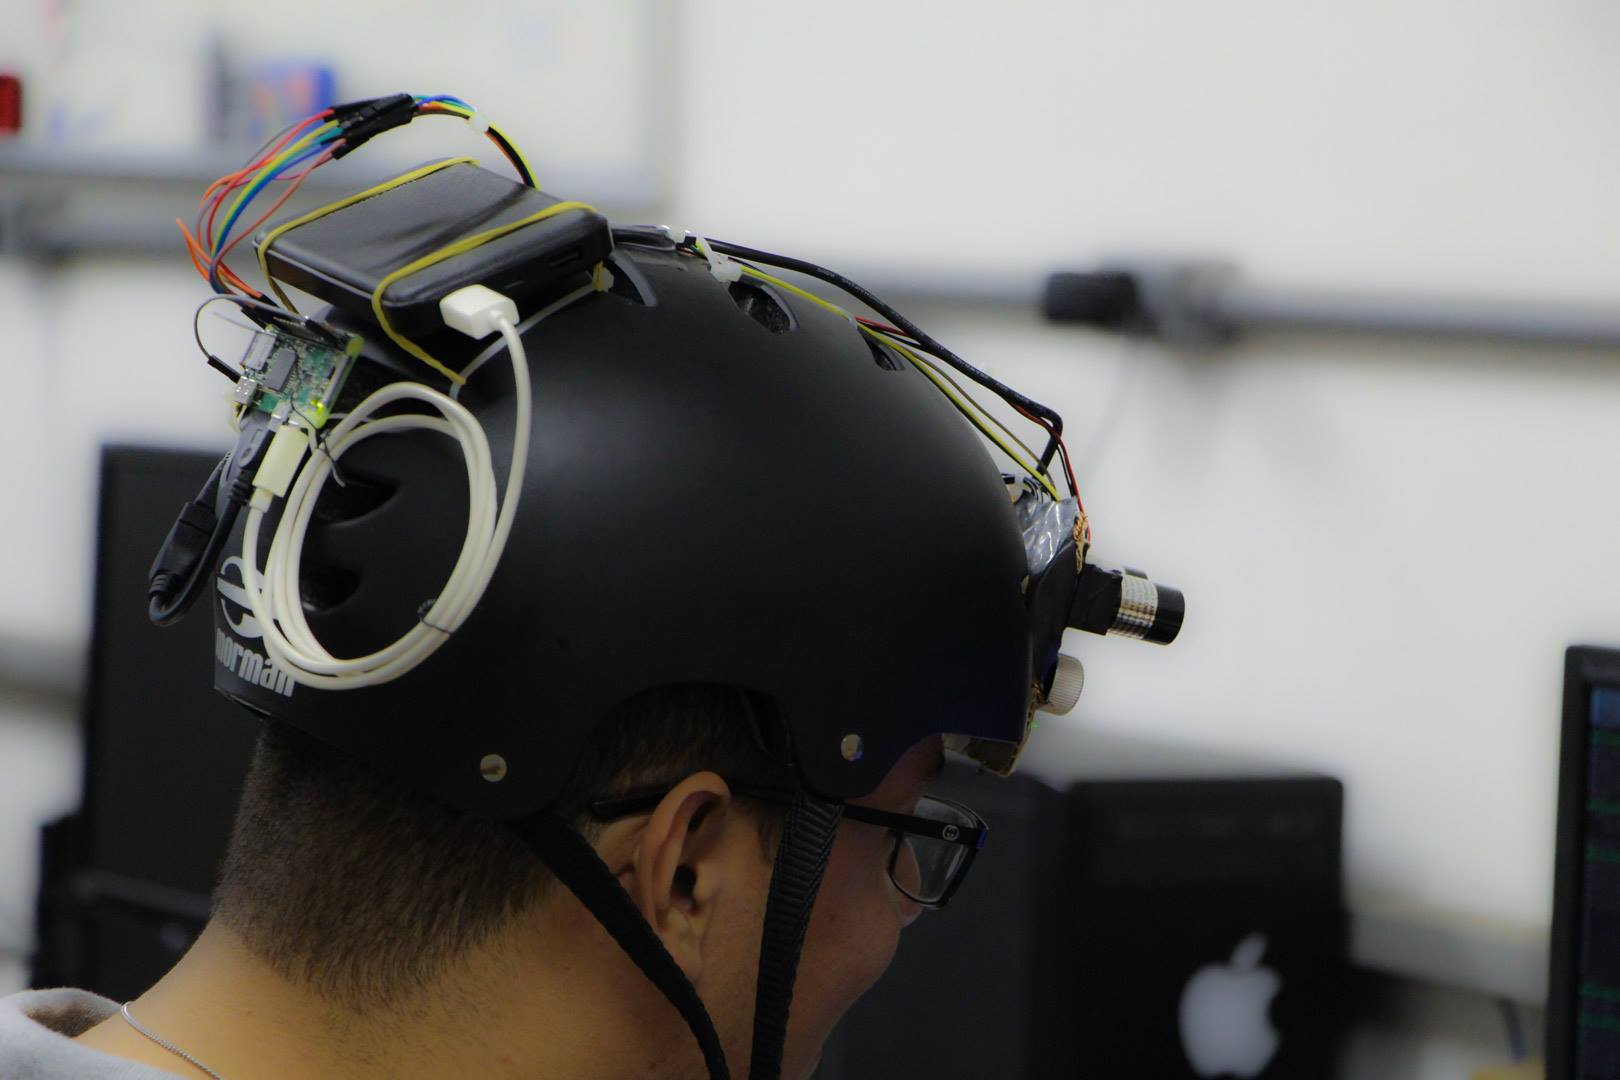
\includegraphics[width=\linewidth]{Figures/prototype2.jpg}  
  \caption{User wearing the device}
  \label{fig:wearing}
\end{subfigure}
\caption{Prototype Assembled}
\label{fig:Prototype}
\end{figure}

The wearable prototype is depicted in Figure~\ref{fig:Prototype}. Figure~\ref{fig:proto} displays a three-dimensional representation of the device, showing both the front and side views. Figure~\ref{fig:wearing} depicts a user wearing the device as seen from the rear. The hardware is equipped with a LIDAR sensor that is attached to a processing unit for accurately measuring the distance and estimating the 3D geometry of the objects being sensed. A Raspberry Pi Zero W was selected as the device for processing unit data, with power supplied by a 5V battery. During the development process, we took into account both the specifications for the wearable device and the needs for its use.

We utilized this prototype to do specific operations within this domain. Having already verified the sensing features of this system, our primary focus in this study was to conduct tests specifically evaluating its computational capability. Subsequent experiments have demonstrated that this prototype is capable of doing certain intended tasks, but its capabilities are restricted when confronted with more demanding processing requirements. Therefore, this viewpoint provides a rational basis for supporting the proposed Edge-based design. In the subsequent part, we will elaborate on the procedure of selecting the hardware for Edge Computing.

\paragraph{Edge AI server Node - Hardware selection and integration}

In addition to the smart helmet, another crucial component of the overall system is the Edge AI server node. Therefore, the hardware selection must take into account portable embedded systems that can facilitate machine-to-machine communication for this particular stage. Our case study focuses on implementing machine learning techniques within the setting of WBAN/WLAN to develop a viewpoint on Wearable Edge AI. This paper presents a comparison of the performance of four hardware components that have the capability to provide this utility.

\begin{figure}[h!]
    \centering
    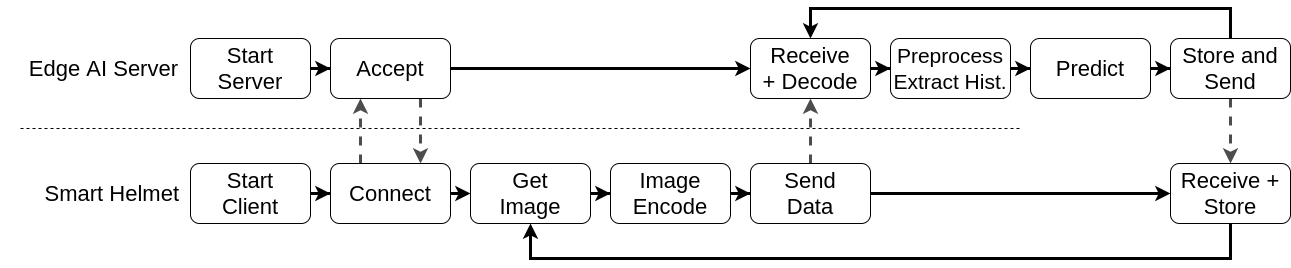
\includegraphics[width=\linewidth]{Figures/pipeline-Edge-AI.png}
    \caption{Edge AI service pipeline. In the proposed architecture, clients perform part of the processing, while the AI pipeline is provided by the Edge AI server node.}
    \label{fig:pipeline-edge-ai}
\end{figure}

Initially, we established a pipeline that separates the components which are processed locally from those processed within the Edge AI server node. At first, the local systems obtain and convert the image, transmitting the converted data to the edge server. Within this server, the application initializes a trained machine learning model and continuously receives encoded frames. It then proceeds to decode, preprocess, and extract the pseudospectrum from these frames, thereafter evaluating it. The assessment outcome is thereafter stored by the Edge AI server and returned to the device for duplication. The diagram in Figure \ref{fig:pipeline-edge-ai} illustrates the suggested pipeline for the Edge AI server, which is designed to accommodate a solitary client.

We evaluated multiple devices for developing the solution. In the context of this Wearable Edge AI solution, we evaluated the Raspberry Pi Zero W, Raspberry Pi 3B, Raspberry Pi 3B+, and Jetson Nano platforms as potential options for delivering Edge AI functionality. These solutions are all commercially available ARM-based computer-on-modules.

\subsubsection{Edge AI Software}

As stated in the introduction, the condition of leaves serves as crucial indicators of the overall health of the ecosystem. Therefore, we opted to assess the limitations of an Edge AI component that conducts leaf classifications into two categories: "normal" and "diseased." This section delves into the implementation of Edge AI software as demonstrated in the case study.

\begin{figure}[h!]
    \centering
    \includegraphics[width = .9\linewidth]{Figures/leaves.png}
    \caption{Sample of healthy and diseased leaf images obtained from the dataset.}
    \label{fig:healthy-and-diseased-leaves}
\end{figure}

\begin{figure}[h!]
    \centering
    \includegraphics[width=.9\linewidth]{Figures/pipeline.png}
    \caption{Data processing pipeline and associated substages. For the image extraction, the associated stages are the color space conversion and histogram extraction.}
    \label{fig:pipeline}
\end{figure}

To begin, it is essential to locate a dataset that contains comparable information to the required dataset. After conducting thorough research, we have chosen to utilize the dataset provided by Chouhan, Kaul, and Singh in their publication on leaf diseases \cite{leaf-disease-dataset}. The authors provide a dataset consisting of 4,503 photos depicting leaves exhibiting both healthy and diseased conditions. Out of this collection, there are 2,278 photographs depicting healthy leaves, whereas 2,225 images show damaged leaves. There are 12 distinct species represented by the leaves. Figure \ref{fig:healthy-and-diseased-leaves} showcases photos of both healthy and diseased leaves extracted from the original dataset. 

The designers of this database ensure a clear distinction between infected and healthy leaves. Any variation in hue and texture is solely attributable to illness in all instances. The photos had a pixel resolution of 6,000x4,000. In order to enhance the test's speed and align the resolution with that of commonly used cameras in embedded systems, we reduced the resolution to 900x600 pixels. The improved resolution is equivalent to 15\% of the original size.
	
The data extraction and classification method adheres to a traditional pipeline. Initially, we obtain the image and then proceed to extract a feature vector. Next, we employ a machine learning model to categorize the image based on its attributes, resulting in a binary classification outcome. The pipeline is depicted in Figure \ref{fig:pipeline}, illustrating the substages linked to each primary stage.

\begin{figure}[h]
    \centering
    \includegraphics[width=.9\linewidth]{Figures/pseudospectrum-distribution.png}
    \caption{Pseudospectrum extraction samples}
    \label{fig:pseudospectrum}
\end{figure}

Within this particular framework, our method to addressing this issue involves the development of a pseudospectral analytic system \cite{iceis21orange}. In this process, the feature vector is a \textit{pseudospectrum}, which is obtained by extracting the histogram from the Hue channel in the HSV color space. Ultimately, the histogram is divided by its total sum, resulting in a probability density function (PDF) that represents the distribution of colors. This PDF is then referred to as the pseudospectrum. Figure \ref{fig:pseudospectrum} illustrates several instances of the extraction of pseudospectra.

\begin{figure}[h!]
    \centering
    \includegraphics[width = .7\linewidth]{Figures/neuralnetwork-1.png}
    \caption{\color{black}Neural network representation. The chosen model was a Multi-Layer Perceptron (MLP). All layers are fully connected. The number beneath the blocks represents the number of neurons in each layer.}
    \label{fig:neural-network}
\end{figure}

Subsequently, a neural network is employed to categorize the leaf. In this instance, we employed a conventional Multi-Layer Perceptron (MLP) model to carry out the computations. Despite the model's lack of novelty, we selected it due to its simplicity, which results in improved performance on low-power devices in Edge Computing. Despite its simplicity, the model has demonstrated intriguing outcomes in the classification of citrus fruits \cite{iceis21orange}. Within this particular framework, we employed a network that received 256 inputs derived from the pseudospectrum. The network's hidden layers consisted of 128, 64, 32, 16, and 8 neurons, respectively. The result yielded a binary categorization of either healthy or diseased. Figure \ref{fig:neural-network} presents a concise representation of the network's structure.

\begin{figure}[h!]
    \centering
    \includegraphics[width = .7\linewidth]{Figures/loss_function.png}
    \caption{Loss function during the training process}
    \label{fig:loss_function}
\end{figure}

The \textit{scikit-learn} framework was employed to construct our model \cite{pedregosa2011scikit}. The training was conducted using a backpropagation technique, employing a cross-entropy loss function. For the purpose of training, we partitioned the original dataset of photos into two distinct subsets. During the initial phase, we employed a random selection process to choose 10\% of the photos depicting both damaged and healthy leaves from each species. These selected images were then used to create a test dataset. The remaining 90\% constituted a training set. Our system was trained using 90\% of the photos from the training set, while the remaining 10\% were used for validation. The behavior of the cross-entropy loss during the training is depicted in Figure \ref{fig:loss_function}. This training concludes when the cross-entropy loss value does not improve by more than $10^{-5}$ for ten consecutive epochs, as determined by an arbitrary convergence criteria.

In addition to this model, we also evaluated the feasibility of utilizing a convolutional neural network (CNN) model for making predictions on the embedded hardware. This method is more contemporary, although necessitates a greater amount of computer capacity. Therefore, we put forward a test that assessed two aspects:


\begin{itemize}
    \item How much improvement can a CNN obtain over an Computer Vision and MLP.
    \item How much performance the embedded system loses using this method over a traditional approach.
\end{itemize}

We created a simple CNN model that approaches this process. Figure \ref{fig:CNN-model} displays an illustration of this model.

This model utilizes five 2D-convolutional layers in the feature extraction stage. The layers have 16, 32, 64, 64, and 64 filters of size 3x3, respectively. Following each convolutional layer, there is a further max pooling layer with a 2x2 size. Following these phases, the output is compressed and sent through a dense layer consisting of 1024 neurons. So far, the convolutional and dense layers have employed a rectified linear unit (ReLU) activation function. Ultimately, the result is a solitary neuron that utilizes a sigmoid activation function. The loss function employed was the cross-entropy. The function was trained for a total of 12 epochs, a value determined empirically as the maximum number of epochs to prevent overfitting indications. In addition, we conducted tests on this model based on the hardware and software performance indicators in order to address the problems that were highlighted.

\begin{figure}[h!]
    \centering
    \includegraphics[width = \linewidth]{Figures/CNN_Sensors.png}
    \caption{Proposed CNN model. The convolutional layers have 3x3 filters, with 2x2 pooling. The output is a single value obtained from a sigmoid activation function.}
    \label{fig:CNN-model}
\end{figure}

\begin{figure}[h!]
    \centering
    \includegraphics[width=\linewidth]{Figures/cnn_train_validation.png}
    \caption{Values for accuracy and loss functions in the CNN training process.}
    \label{fig:cnn-train}
\end{figure}

\subsection{Validation Tests}

Once we have put forth the hardware, software, and architectural components, it is essential to set metrics to verify the effectiveness of each stage. Within this area, we present the modeling and metrics utilized to assess each individual component. We assessed the performance of the Edge AI server across different platforms, focusing on the hardware components. We analyzed the metrics of the machine learning software predictions for the suggested application in order to evaluate its software features. Regarding the design, we analyzed the timing limitations for numerous clients linked to the Edge AI server, taking into account a Real-Time Quality of Service (QoS) assessment.

\subsubsection{Hardware Validation Tests}

This appliance consists of two primary hardware components: a Smart-Helmet and an Edge AI server node. The helmet was originally designed to provide versatile applications in this field. Hence, the validation stage deems it imperative to validate the newly introduced component: the Edge AI node. 

In Figure \ref{fig:pipeline-edge-ai}, we delineated the specific functions carried out by both the intelligent helmet and the Edge AI node. Initially, we must assess the hardware components for each of the recommended solutions based on the distributor websites associated with them. The available options include of the Raspberry Pi Zero W, Raspberry Pi 3B, Raspberry Pi 3B+, and Jetson Nano. Table \ref{tab:hardware-specs} presents the most relevant aspects about each solution.

\begin{table}[h!]
\centering
\caption{Hardware Specifications for the Edge AI server node candidates.}
\label{tab:hardware-specs}
\resizebox{\linewidth}{!}{%
\begin{tabular}{lllll}
\multicolumn{1}{l|}{} & \textbf{Raspberry Pi Zero W} & \textbf{Raspberry Pi 3B} & \textbf{Raspberry Pi 3B+} & \textbf{Nvidia Jetson Nano} \\ \hline \hline
\multicolumn{1}{l|}{\textbf{CPU}} & \begin{tabular}[c]{@{}l@{}}1x ARM11 \\ @ 1GHz\end{tabular} & \begin{tabular}[c]{@{}l@{}}4× ARM Cortex-A53 \\ @ 1.2GHz\end{tabular} & \begin{tabular}[c]{@{}l@{}}4× ARM Cortex-A53 \\ @ 1.4GHz\end{tabular} & \begin{tabular}[c]{@{}l@{}}4x ARM Cortex-A57\\ @ 1.43 GHz\end{tabular} \\ \hline
\multicolumn{1}{l|}{\textbf{RAM}} & 512 MB & 1GB & 1GB & 4GB \\ \hline
\multicolumn{1}{l|}{\textbf{Storage}} & MicroSD card & MicroSD card & MicroSD card & MicroSD card \\ \hline
\multicolumn{1}{l|}{\textbf{\begin{tabular}[c]{@{}l@{}}Nominal\\ Power\end{tabular}}} & \begin{tabular}[c]{@{}l@{}}5V over microUSB\\ (max. 6W)\end{tabular} & \begin{tabular}[c]{@{}l@{}}5V over microUSB\\ (max. 12.5W)\end{tabular} & \begin{tabular}[c]{@{}l@{}}5V over microUSB\\ (max. 12.5W)\end{tabular} & \begin{tabular}[c]{@{}l@{}}5V over P4 Jack Barrell\\ (max. 5W/20W modes)\end{tabular} \\ \hline
\multicolumn{1}{l|}{\textbf{\begin{tabular}[c]{@{}l@{}}Network\\ Platform\end{tabular}}} & 2.4GHz 802.11n & 2.4GHz 802.11n & \begin{tabular}[c]{@{}l@{}}2.4GHz/5GHz \\ 802.11b/g/n/ac\end{tabular} & \begin{tabular}[c]{@{}l@{}}2.4GHz \\ 802.11n \\ (over USB)\end{tabular}
\end{tabular}%
}
\end{table}

To conduct this test, we execute the tasks outlined in the pipeline depicted in Figure \ref{fig:pipeline-edge-ai} for every candidate. We assess the time delay required to complete all internal phases for each solution, executing identical code to receive input from a client, make predictions about the outcome (whether it is healthy or unhealthy), return the predictions, and store them in a text file. During the hardware evaluation, we just focus on the latency of the steps that are executed locally. The components of the system that rely on networking will be executed at a later time, taking into account the characteristics of the architecture. Additionally, we conducted a comparison of the two software techniques by testing the ratio of average predictions per second. This addresses one of the inquiries posed in the software proposal, namely evaluating the efficacy of the model on the embedded hardware.

\subsubsection{Software Validation Tests}

The unique software being presented is a machine learning-based prediction system that operates on an Edge AI server node. To address this issue, we utilized a Multilayer Perceptron (MLP) neural network model to accurately forecast whether leaf images exhibit signs of disease or are in a healthy state. Furthermore, we conducted an evaluation of the same measures for the CNN model in order to validate the enhancement in this characteristic by employing a more contemporary approach.

In order to successfully validate the program, it is imperative that we thoroughly comprehend the performance of this machine learning model in relation to the specific data at hand. Therefore, we employ conventional machine learning metrics to examine the data. We evaluate the confusion matrix, as well as the \textit{Precision}, \textit{Recall}, and \textit{F1-Score} metrics. The subsequent equations illustrate the formulas for various measures. The above equations define the variables as follows: $TP$ represents the count of true positives, $FP$ represents the count of false positives, $TN$ represents the count of true negatives, and $FN$ represents the count of false negatives.

\begin{equation} \label{eq1}
\begin{split}
Precision =  \frac{TP}{TP + FP} \\
\end{split}
\end{equation}

 \begin{equation} \label{eq2}
\begin{split}
Recall =  \frac{TP }{TP +FN} \\
\end{split}
\end{equation}

\begin{equation} \label{eq3}
\begin{split}
F1\text{-}Score = 2 \times \frac{Precision \times Recall}{Precision + Recall} \\
\end{split}
\end{equation}

\subsubsection{Architecture Validation Tests}

It is necessary to take into account characteristics that assess the individual and overall performance of the proposed scenario for the validation tests of the architecture. Therefore, we devised an experiment that was specifically designed as a Real-Time Quality of Service (QoS) test, drawing inspiration from previous research on IoT and Wireless Sensor Networks \cite{silva2019analyzing,iceis21dt}, with the aim of assessing the real-time constraint. This assessment assesses the proficiency in completing a series of tasks, taking into account both individual and network-related circumstances. 

At first, we consider duration as discrete intervals, as the set $D = d_i,  i \in \mathbb{N}$, where $d_{i+1} - d_i = \theta$, and $\theta$ is a constant sampling time. The soft real-time deadline will be represented by $\phi$, where $\phi = k \times \theta, k \in \mathbb{N}^*$. Thereby, we establish the following definitions:

\begin{definition} 
    Let $D = d_i$ be the finite set of nodes performing IoT-dependant tasks, where $i \in \mathbb{N}$;
\end{definition}

\begin{definition}
    Let $E = e_i$ be the finite set of events that each node performs, where $i \in \mathbb{N}$;
\end{definition}

\begin{definition}
    Let $L = l_{g,e}$ be the length of time interval that the node $g$ takes to perform an event $e$ during the execution, where $g \in G$ and $e \in E$;
\end{definition}

\begin{definition}
    Let $P = p_{i}$ be the set of patterns of events to be observed in the devices, where $p_i = E_i$, $E_i \subset E$ and $i \in \mathbb{N}$. In this case, all client devices will perform the same events in the same pattern;
\end{definition}

\begin{definition}
    Let $O = o_{i}$ be the finite set of observations of a certain pattern $p_i \in P$ on each device;
\end{definition}

The equation that represents the elapsed time $\lambda$ to observe a particular pattern $p_i \in P$ is:

\begin{equation}
    \lambda_{o_i} = \sum l_{g,e_k} | \forall e_k \in o_i, o_i = O_{p_i}
\end{equation}

All client devices in the network composition will have the same $\phi$ soft real-time deadline. Given this equation, let $\hat{O}$ be a subset of $O$, where $\lambda_{o_i} \leq \phi$, $\forall o_i \in \hat{O}$. Finally, given the sets $O$ and $\hat{O}$:

\begin{definition}
    Let $N$ be the number of elements on the set $O$;
\end{definition}

\begin{definition}
    Let $N_h$ be the number of elements on the subset $\hat{O}$;
\end{definition}

The quality factor $Q_f$ will be represented by the following equation:

\begin{equation}
    Q_f = \frac{N_h}{N} (\times 100 \%)
\end{equation}

This result represents how often the nodes execute a pattern of events without violating the soft real-time constraints. The clients represent the smart-helmets and will send data to the Edge AI server node in parallel on each test. 

\subsubsection{Case Study Validation for Deployment}

In order to verify the system in the case study, we employed a test that relied on the probability distribution function outlined in Equation \ref{eq:pdf}. The equation represents the likelihood of encountering damaged leaves during a sample procedure near the tree, as determined by the spatial coordinates. The function's maximum value is determined by the $P_0$ value, and the spatial location of the disease's epicenter is given by the $(x_0, y_0, z_0)$ coordinate. The situation is depicted in Figure \ref{fig:canopy-disease-spread}.

\begin{figure}[h!]
    \centering
    \includegraphics[width = .8\linewidth]{Figures/pin-cylinder-test.png}
    \caption{Sampling process illustration}
    \label{fig:pin-cylinder-test}
\end{figure}

For this validation test, we examine a group of three climbers who collect leaf samples at different heights inside certain areas of the canopy called transects. The whereabouts of the three climbers are arbitrary but known. Additionally, the locations of the stops along the transect are known, enabling the mapping of their positions as three-dimensional points during the procedure. The researchers should be positioned within a random radius from the center of the tree trunk in the canopy to achieve a more optimal spatial dispersion.  The organization for a 5-meter-radius and 9 stops is depicted in Figure \ref{fig:pin-cylinder-test}.

We examined a procedure that allows for an arbitrary number of stops during the ascent, in accordance with the requirements of the transect method. During each stop, the researcher would collect samples of leaf images. The system autonomously categorizes the sampled leaves as either healthy or unhealthy based on the acquired methodology. Consequently, for every $(x,y,z)$ coordinate at which a researcher employs the helmet and a backdrop template to sample the leaves, the system is capable of computing the proportion of unhealthy entities. 

For climbers to take tiny goods to the canopy, we suggest using a background template. This template is a sturdy object with identification tags placed along its edges. This suggestion enables the algorithm to circumvent any influence from the background during the sampling procedure. We created a preliminary examination to showcase this problem utilizing the wearable camera. The prototype captures the image, detects specific tags within the backdrop template, applies a four-point transformation to isolate the region of interest, and utilizes Otsu's binarization technique to segment the image. The pipeline utilized in this investigation is depicted in Figure \ref{fig:segmentation}.

\begin{figure}[h!]
    \centering
    \includegraphics[width = .9\linewidth]{Figures/segmentation.png}
    \caption{Demonstration of the segmentation process. The prototype used a USB camera to capture the data, which can be processed by the prototype itself or in the Edge AI server node.}
    \label{fig:segmentation}
\end{figure}

Using this data, the system does a regression analysis to fit the probability density function (PDF) outlined in Equation \ref{eq:pdf}. To address this issue, it is necessary to acquire the parameters contained in the tuple $T = (p_0, \sigma, x_0, y_0, z_0)$. We opted to employ an Evolutionary Algorithm for the execution of this task, whereby the tuple candidates are regarded as the genotype and the mean squared error serves as the fitness function. {The decision was made considering three primary factors:}  

\begin{itemize}
    \item \textit{Ease of use:} it is easier to perform regression for a smooth parametric arbitrary three-dimensional distribution function with an evolutionary algorithm than designing an interpolation based in various parameters and kernel functions;
    \item \textit{Flexibility:} the same process can be used to obtain a regression to any parametric model by just changing the input parameters on the same algorithm;
    \item \textit{Robustness:} The regression algorithm displayed robust results, even with a change on its parameters.
\end{itemize}

In this case, the climbers would make nine stops, collecting 200 leaves at each stop. The system autonomously categorizes every leaf, transmitting data regarding each position and the compressed image of the leaf. To simulate the sampling process, we randomly selected 100 photos from the original dataset. Our selection approach utilizes a random number and evaluates its compatibility with the probability density function (PDF) defined by Equation \ref{eq:pdf} using arbitrary parameters. The value of $p_0$ was selected as $0.65$, taking into account the highest occurrence of sick leaves observed in the study conducted by García-Guzman et al. \cite{garcia2004incidence}. Furthermore, we established the coordinates of the tree stem and ground as the origin $(0,0,0)$ and deliberately chose $(2,-2,8)$ as the epicenter of the sickness. Ultimately, the value of our standard deviation ($\sigma$) was $5$. Therefore, the ultimate random PDF for this exam is:

\begin{equation}
\label{eq:arb-pdf}
    P(x,y,z) = 0.65 . e^{-\frac{(x-2)^2 + (y+2)^2 + (z-8)^2}{10}}
\end{equation}

Ultimately, the system categorizes and archives the data relative to the image. Our intention is to utilize the saved data to conduct an analysis that will yield the original PDF values through the implementation of an evolutionary algorithm. The Edge AI node is capable of conducting this analysis to offer on-site insights derived from the collected data. The goal is to approximate the original values of Equation \ref{eq:arb-pdf} as accurately as possible. Figure \ref{fig:arb_pdf} illustrates the spatial distribution of the disease in the given arbitrary function. The likelihood of encountering diseased leaves at this position increases as the red circle becomes larger and more vibrant in color. The brown stick denotes the location of the primary tree trunk.

\begin{figure}[h!]
    \centering
    \includegraphics[width = .7\linewidth]{Figures/arb-pdf.png}
    \caption{Arbitrary PDF display. The larger and more colorful red dots have a bigger probability density. {\color{black}The brown cylinder represents the main tree trunk.}}
    \label{fig:arb_pdf}
\end{figure}

%%%%%%%%%%%%%%%%%%%%%%%%%%%%%%%%%%%%%%%%%%
\subsection{Results}

The preceding part provided a comprehensive overview of the hardware, software, and architecture components utilized in the proposed case study. In addition, we presented the assessment criteria employed to validate each branch of the co-design reviewed pattern. Ultimately, we deliberated on the verifications required for an application in the given case study. This section presents the results received from experiments conducted on the proposed elements.

\subsubsection{Hardware Validation Tests}

We present the hardware specifications for the Edge AI server node. All candidates are COTS computer-on-modules. To validate the hardware candidate, we assessed the candidates' performance in executing the internal Edge AI tasks. The pipeline for the proposed test is illustrated in Figure \ref{fig:hwtest-pipeline}. The internal duties for the Edge AI server are categorized into three stages: (i) preprocessing and extracting the feature vector, (ii) predicting the leaf condition, and (iii) storing the prediction data. 

\begin{figure}[h!]
    \centering
    \includegraphics[width = .7\linewidth]{Figures/hw-test-pipeline.png}
    \caption{Pipeline for the hardware validation test.}
    \label{fig:hwtest-pipeline}
\end{figure}

We conducted the tests on all the candidates listed in Table \ref{tab:hardware-specs}. We conducted tests on the Jetson Nano in both the 5W and 20W power modes. We executed the subsequent pipeline on all 437 photos from the test set. The hardware candidates and configurations will be referred to as follows: \textit{Zero W} (Raspberry Pi Zero W), \textit{3B} (Raspberry Pi 3B), \textit{3B+} (Raspberry Pi 3B+), \textit{Jetson 5W} (Jetson Nano operating in 5W mode), and \textit{Jetson 20W} (Jetson Nano operating in 20W mode).

The Zero W was evaluated as it serves as the computer in the helmet prototype. The \textit{3B} and \textit{3B+} models were evaluated due to their lower pricing compared to the Jetson Nano, although having similar processor configurations. Using the \textit{Jetson 5W}, our goal is to compare the candidate with the highest cost but with limited hardware capabilities. In this economic operation mode, the operating system disables half of the CPU cores to conserve power. Ultimately, our objective was to confirm the disparity in performance between the priciest gear in the most powerful operational state and the performance of the other contenders.

\begin{figure}[h]
    \centering
    \includegraphics[width = .8\linewidth]{Figures/HW-stage1.png}
    \caption{Latency results for the first stage.}
    \label{fig:hw-stage1}
\end{figure}

Initially, we assessed the outcomes for Stage 1. During this stage, the hardware does preprocessing on the image by converting its color space from RGB to HSV. Next, it retrieves the pseudospectrum from the Hue channel. The latency evaluation findings from the first stage are presented in Figure \ref{fig:hw-stage1}. The \textit{Zero W} device completed the first stage in $107.61 \pm 2.53$ ms. The \textit{3B} device took $15.34 \pm 0.28$ ms to perform this task. The \textit{3B+} device took $29.69 \pm 0.13$ ms to complete this stage. The \textit{Jetson 5W} device took $11.47 \pm 0.87$ ms to perform this part, while the \textit{Jetson 20W} device took $9.32 \pm 0.81$ ms.

\begin{figure}[h]
    \centering
    \includegraphics[width = .8\linewidth]{Figures/HW-stage2.png}
    \caption{Latency results for the second stage.}
    \label{fig:hw-stage2}
\end{figure}

Then, we assessed the results for the Stage 2. This stage corresponds to the prediction of the leaf condition using the model. Figure \ref{fig:hw-stage2} presents the results obtained from the evaluation of the latency from the second stage. \textit{Zero W} took $15.62 \pm 0.98$ ms to perform the first stage, \textit{3B} took $3.01 \pm 0.07$ ms to perform this task, \textit{3B+} took $5.66 \pm 0.10$ ms to perform this stage, \textit{Jetson 5W} took $2.52 \pm 0.14$ ms to perform this part, and \textit{Jetson 20W} took $1.71 \pm 0.09$ ms.

\begin{figure}[h]
    \centering
    \includegraphics[width = .8\linewidth]{Figures/HW-stage3.png}
    \caption{Latency results for the third stage.}
    \label{fig:hw-stage3}
\end{figure}

At last, we analyzed the outcomes pertaining to Stage 3. This stage pertains to the retention of the information acquired from the preceding stages. The latency evaluation results from the second stage are depicted in Figure \ref{fig:hw-stage3}. The \textit{Zero W} required 0.07 ± 0.05 milliseconds to complete the initial stage. The \textit{3B} took 0.02 ± 0.04 milliseconds to accomplish this task. The \textit{3B+} required 0.03 ± 0.05 milliseconds to perform this stage. The \textit{Jetson 5W} took 0.02 ± 0.04 milliseconds to complete this part, whereas the \textit{Jetson 20W} took 0.01 ± 0.03 milliseconds. The observed discrepancies in this instance arose due to the time interval of this particular stage being shorter than the minimum recorded value, resulting in numerous measurements being conducted within an infinitesimally little timeframe.

All of the suggested gear is capable of executing the intended task. Therefore, the decision is made by assessing the performance, which may be subsequently compared to the project cost. Based on the test findings, it is evident that the Jetson Nano outperformed the Raspberry Pi 3B and 3B+ even when operating in power saving mode. The Raspberry Pi Zero W has the least amount of computational capacity, resulting in the poorest overall performance. Despite the similarities in hardware specs, the Raspberry Pi 3B outperformed the Raspberry Pi 3B+ and exhibited a performance level similar to the Jetson Nano operating in the 5W mode. The graph labeled as Figure \ref{fig:predpersec} illustrates the mean anticipated rate of predictions per second for each platform.

\begin{figure}[h]
    \centering
    \includegraphics[width = .8\linewidth]{Figures/predpersec.png}
    \caption{Average expected predictions per second ratio on each platform. The number in blue displays the expected ratio.}
    \label{fig:predpersec}
\end{figure}

As anticipated, the performance of the \textit{Zero W} was exceedingly poor. This supports the initial architectural idea to include an additional hardware component to handle the more demanding processing activities. Another anticipated outcome was the attainment of the highest level of performance using Jetson 20W. A notable finding is that, despite having a potentially superior processor, \textit{3B} exhibited significantly better performance than \textit{3B+}. Another significant finding is that despite disabling two out of the four cores, the \textit{Jetson 5W} exhibited higher performance compared to the \textit{3B} and \textit{3B+} models operating with all four cores and consuming over twice the amount of power. Given its ability to execute at a high level while operating under a power constraint, the \textit{Jetson 5W} is an excellent choice for field processing. Based on these findings, we conclude that \textit{3B} and \textit{Jetson 5W} are the primary contenders for fulfilling this application, as they exhibit the most favorable balance between performance and power consumption.

Ultimately, we assessed the ratio of average predictions per second by executing the CNN and MLP pipelines. The sole distinction in the CNN pipeline, as depicted in Figure \ref{fig:hwtest-pipeline}, is the absence of a feature extraction procedure, which is not necessary for the CNN. Therefore, this stage alone encompasses the alteration of input data to be provided to the model. The tests were conducted on the primary hardware options, namely Jetson 5W, Jetson 20W, and pi3B. The findings achieved for the predictions per second in the proposed setups were as follows:

\begin{itemize}
    \item The average predictions per second ratio in pi3B was $54 \pm 1$ for the MLP pipeline and $5 \pm 0$ for the CNN pipeline; \item The average predictions per second ratio in Jetson 5W was $71 \pm 5$ for the MLP pipeline and $10 \pm 0$ for the CNN pipeline;
    \item The average predictions per second ratio in Jetson 20W was $91 \pm 7$ for the MLP pipeline and $15 \pm 0$ for the CNN pipeline;
\end{itemize}

Figure \ref{fig:cnn-mlp-comp} also displays these results in the respective cited order. This data indicates that even in case of improvements on the software results, the CNN model is not adequate for time-restrictive tasks in the proposed configurations. This model is suitable to perform a later review of in-field captured results, but not to be integrated into a distributed constrained environment within the context of these tests.

\begin{figure}[h!]
    \centering
    \includegraphics[width = .32\linewidth]{Figures/pps-pi3B.png}
    \includegraphics[width = .32\linewidth]{Figures/pps-j5.png}
    \includegraphics[width = .32\linewidth]{Figures/pps-j20.png}
    \caption{MLP and CNN performance comparison test results.}
    \label{fig:cnn-mlp-comp}
\end{figure}

\subsubsection{Software Validation Tests}

The software validation tests in the previous section incorporate conventional ML metrics. Within this particular framework, we assessed the metrics of \textit{Precision}, \textit{Recall}, and \textit{F1-Score}. 

To ensure simplicity, the validation set is randomly selected from the training data only once. It contains 10\% of the total photos from the training data. The findings for the validation set are shown in Table \ref{tab:res-training}. The findings indicate that the system successfully detected the sick leaves in 90\% of the instances. Additionally, the Precision and Recall exhibit equilibrium, leading to a well-balanced F1-Score. This outcome suggests that the number of incorrect positive and negative results is almost equal. The confusion matrix obtained from this stage is displayed in Table \ref{tab:cfmat-valid}.

\begin{table}[h!]
\centering
\caption{Metric results for the validation dataset. This set was obtained separating 10\% of the training data for validation.}
\label{tab:res-training}
\resizebox{.6\linewidth}{!} \\ \hline
 & Precision & Recall & F1-Score & Support \\ \hline
healthy & 0.89 & 0.90 & 0.90 & 198 \\
diseased & 0.90 & 0.90 & 0.90 & 209 \\ \hline
\end{tabular}%
}
\end{table}

\begin{table}[h!]
\centering
\caption{Confusion Matrix for the validation data}
\label{tab:cfmat-valid}
\resizebox{.4\linewidth}{!}{%
\begin{tabular}{l|l|l|}
\cline{2-3}
 & \textbf{Healthy} & \textbf{Diseased} \\ \hline
\multicolumn{1}{|l|}{\textbf{Healthy}} & 178 & 20 \\ \hline
\multicolumn{1}{|l|}{\textbf{Diseased}} & 21 & 188 \\ \hline
\end{tabular}%
}
\end{table}

Additionally, we computed the global mean and the conventional metrics for the test dataset. Previously, the test set was partitioned by extracting 10\% of the photos from the original dataset. The acquired results for the validation set are shown in Table \ref{tab:res-test}, while the confusion matrix for this stage is displayed in Table \ref{tab:cfmat-test}. Once again, the results indicate that the system was able to accurately detect the sick leaves in approximately 90\% of the cases. Despite a slight disparity, the Precision and Recall exhibit equilibrium, leading to a harmonized F1-Score. This outcome validates the practicality of the suggested method within the specified framework.

\begin{table}[h!]
\centering
\caption{Metric results for the test dataset. This set previously separated, taking 10\% of all images.}
\label{tab:res-test}
\resizebox{.6\linewidth}{!} \\ \hline
 & Precision & Recall & F1-Score & Support \\ \hline
healthy & 0.93 & 0.88 & 0.91 & 217 \\
diseased & 0.89 & 0.93 & 0.91 & 220 \\ \hline
\end{tabular}%
}
\end{table}

\begin{table}[h!]
\centering
\caption{Confusion Matrix for the test data}
\label{tab:cfmat-test}
\resizebox{.4\linewidth}{!}{%
\begin{tabular}{l|l|l|}
\cline{2-3}
 & \textbf{Healthy} & \textbf{Diseased} \\ \hline
\multicolumn{1}{|l|}{\textbf{Healthy}} & 192 & 25 \\ \hline
\multicolumn{1}{|l|}{\textbf{Diseased}} & 15 & 205 \\ \hline
\end{tabular}%
}
\end{table}

Based on these stages, we can infer that the method is valid for the intended purpose. It accurately distinguishes between diseased and healthy leaves with an approximate accuracy of 90\%, and the outcomes are well-balanced. The following tests must verify the architectural characteristics of this solution. In addition, we conducted identical predictions taking into account the CNN. In this case, we utilized the identical test set to acquire the prediction outcomes.

\begin{table}[h!]
\centering
\caption{Metric results for the test dataset - CNN results. This set is the same previously separated for the MLP.}
\label{tab:res-test-cnn}
\resizebox{.6\linewidth}{!} \\ \hline
 & Precision & Recall & F1-Score & Support \\ \hline
healthy & 0.96 & 0.95 & 0.96 & 217 \\
diseased & 0.95 & 0.96 & 0.96 & 220 \\ \hline
\end{tabular}%
}
\end{table}

\begin{table}[h!]
\centering
\caption{Confusion Matrix for the test data - CNN results}
\label{tab:cfmat-test-cnn}
\resizebox{.4\linewidth}{!}{%
\begin{tabular}{l|l|l|}
\cline{2-3}
 & \textbf{Healthy} & \textbf{Diseased} \\ \hline
\multicolumn{1}{|l|}{\textbf{Healthy}} & 207 & 10 \\ \hline
\multicolumn{1}{|l|}{\textbf{Diseased}} & 9 & 211 \\ \hline
\end{tabular}%
}
\end{table}

As expected, the CNN performed better than the MLP. The results exhibit a 5\% enhancement in precision compared to the previous results. This outcome reinforces the necessity of utilizing this approach in future investigations instead of the MLP model. From the standpoint of leveraging greater processing capacity for data analysis, the Convolutional Neural Network (CNN) is a more favorable model compared to the Multilayer Perceptron (MLP).

\subsubsection{Architecture Validation Tests}

The architecture validation test assesses the capacity to execute a task while adhering to a soft real-time limitation. It refers to a performance assessment that offers a comprehensive perspective of the scalability of the suggested architecture. In this case, we employed the Jetson Nano as an Edge AI server to execute the pipeline illustrated in Figure \ref{fig:pipeline-edge-ai}. We designed a version of this system for the client that gives latency statistics for the steps marked in Figure \ref{fig:archtest-dataflow}.

\begin{figure}[h!]
    \centering
    \includegraphics[width = .9\linewidth]{Figures/archtest-dataflow.png}
    \caption{Stages considered in the architectural validation test.}
    \label{fig:archtest-dataflow}
\end{figure}

All clients have access to a uniform set of events. The number of nodes executing the tasks is equivalent to the number of devices carrying out the IoT-dependent operations. This experiment involves augmenting the client count and assessing its impact on the soft real-time restriction.

Thus, it is necessary to initially assess the real-time criteria in relation to the pipeline depicted in Figure \ref{fig:archtest-dataflow}. Therefore, we conducted the test taking into account the latency of the procedures for a solitary customer. Additionally, the test takes into account a series of finite discrete time intervals. Within this framework, we have designated the smallest time interval as 1 millisecond. The delay for each step in a single-client test is shown in Figure \ref{fig:arch-steps-latency}. In order to establish the soft real-time constraint ($\phi$), we assessed the minimum quantity of blocks required to deliver the service to a single client with a 100\% level of quality ($Qf = 1.0$), along with an extra 10\% allowance for loosening the criterion. We established the value of $\phi$ as 90 milliseconds using this approach.

\begin{figure}[h!]
    \centering
    \includegraphics[width = .8\linewidth]{Figures/arch-steps-latency.png}
    \caption{Latency for each of the steps presented in Figure \ref{fig:archtest-dataflow}}
    \label{fig:arch-steps-latency}
\end{figure}

Once $\phi$ was defined, we conducted multiple iterations of the test with 2 to 9 clients, all of whom were assigned the same assignment. The simulations were conducted on a computer machine that was linked to the WLAN network, serving as the Edge Server. During each test, every instance executed the identical test described in Figure \ref{fig:archtest-dataflow}, measuring the duration of each desired occurrence. Ultimately, we calculated the average and standard deviation of the quality factor, taking into account all the nodes that were part of the analysis. The test result is shown in Figure \ref{fig:qf-result}. This outcome demonstrates that the performance of the Edge-AI service deteriorates as the number of customers increases, while adhering to a specific real-time limitation. However, the system maintains a high level of quality despite having a small number of connected clients.

\begin{figure}[h!]
    \centering
    \includegraphics[width = .8\linewidth]{Figures/qf-test.png}
    \caption{Quality Factor test result}
    \label{fig:qf-result}
\end{figure}

Ultimately, we must ascertain whether the degradation in quality was a result of server overload or if other factors had an impact on the simulation program. In this regard, we quantified the mean latency of each stage while progressively increasing the number of nodes. Although steps one and two are contingent on the specific device being used, step three is vulnerable to potential network congestion, and the success of step four hinges on the efficiency of the Edge AI node. The findings for this analysis are displayed in Figures \ref{fig:latency-result-1}, \ref{fig:latency-result-2}, \ref{fig:latency-result-3}, and \ref{fig:latency-result-4}.

As anticipated, the latency in the initial two stages remained unaffected by the growing number of customers. These steps rely solely on the client carrying out its tasks. The third step introduces the initial action that relies on the network. The growing clientele may pose a challenge in the communication process. The findings indicate that this excessive load leads to an increase in delay for this particular stage, albeit the effect on the ultimate outcome is negligible (about 2 milliseconds). Ultimately, stage 4 reveals that the excessive burden on the Edge AI node is the primary element contributing to a decline in quality as the number of clients increases. This level is associated with both networking and the process of machine learning inference.

\begin{figure}[h!]
    \centering
    \includegraphics[width = .8\linewidth]{Figures/latency-st1.png}
    \caption{Latency test results for step 1}
    \label{fig:latency-result-1}
\end{figure}

\begin{figure}[h!]
    \centering
    \includegraphics[width = .8\linewidth]{Figures/latency-st2.png}
    \caption{Latency test results for step 2}
    \label{fig:latency-result-2}
\end{figure}

\begin{figure}[h!]
    \centering
    \includegraphics[width = .8\linewidth]{Figures/latency-st3.png}
    \caption{Latency test results for step 3}
    \label{fig:latency-result-3}
\end{figure}

\begin{figure}[h!]
    \centering
    \includegraphics[width = .8\linewidth]{Figures/latency-st4.png}
    \caption{Latency test results for step 4}
    \label{fig:latency-result-4}
\end{figure}


\subsubsection{Case Study Validation for Deployment}

We additionally conducted a validation phase for the entire solution. To address this issue, we created a simulation based on a case study appliance to test the proposed approach. Within this application, a trio of researchers employ the cylinder approach to sample 200 leaves at various predetermined heights. The Edge AI server node use predictive algorithms to determine the status of each leaf and subsequently records this information alongside the corresponding researcher coordinates. The researchers are positioned within a circular area with a diameter of 5 meters around the tree trunk in this device. Figure \ref{fig:solution-organization} illustrates the arrangement of various devices in relation to the tree trunk.

\begin{figure}[h!]
    \centering
    \includegraphics[width = .7\linewidth]{Figures/case-study-geometry.png}
    \caption{Upper view of the case study organization}
    \label{fig:solution-organization}
\end{figure}

We utilized Equation \ref{eq:arb-pdf} as the reference point for randomly choosing leaves from the sets of infected and healthy samples. Initially, the probability baseline was determined by computing the $(x,y,z)$ coordinate of each researcher at the given position. Subsequently, the computer creates a random number within the interval of $[0,1)$ for each of the 200 samples. If the value is below the baseline probability, the algorithm will choose a diseased leaf. Alternatively, it chooses a nutritious one.

\begin{figure}[h!]
    \centering
    \includegraphics[width = .6\linewidth]{Figures/sampled-disease.png}
    \caption{Case Study sampling distribution. {\color{black}The larger and more colorful red dots have a bigger percentage of diseased leaves. The brown cylinder represents the main tree trunk.}}
    \label{fig:sampling-result}
\end{figure}

After this process, we performed a test with the trained model. The test program uses each sample to estimate the leaf conditions for every device and location. Using this dataset, the application computes the proportion of infected leaves, resulting in a distribution sample. The outcomes of the sampling procedure are depicted in Figure \ref{fig:sampling-result}, taking into account the organization shown in Figure \ref{fig:organization}. As depicted in Figure \ref{fig:arb_pdf}, there is a positive correlation between the size and color intensity of the red dots and the prevalence of diseased leaves.

\begin{figure}[h!]
    \centering
    \includegraphics[width = .6\linewidth]{Figures/regression-pdf.png}
    \caption{Estimated PDF display. The larger and more colorful red dots have a bigger probability density. {\color{black}The brown cylinder represents the main tree trunk.}}
    \label{fig:comparison-pdf}
\end{figure}

Finally, we used an evolutionary algorithm to perform a regression to the parametric PDF presented in Equation \ref{eq:pdf} using the sampled data. Some features of this algorithm are:

\begin{itemize}
    \item Each individual genotype is a $T = (p_0, \sigma, x_0, y_0, z_0)$ tuple;
    \item The population has 100 individuals;
    \item Each round generates 70 offspring (30\% elitism);
    \item Each round has a complementary local search in half the population;
    \item The algorithm stops with a convergence criteria and RMSE lower than 0.05 (5\%);
\end{itemize}

To understand how good would a prediction be, we ran the model 20 times, and evaluated the average value for each paramenter of the $T = (p_0, \sigma, x_0, y_0, z_0)$ obtained from the best individual of the population. The average responses obtained from this experiment are:

\begin{itemize}
    \item $p_0 = 0.65 \pm 0.03$. The original value was $0.65$.
    \item $\sigma = 12 \pm 0.86$. The original value was $5$.
    \item $x_0 = 1.96 \pm 0.21$. The original value was $2$.
    \item $y_0 = -1.52 \pm 0.35$. The original value was $-2$.
    \item $z_0 = 8.1 \pm 0.16$. The original value was $8$.
\end{itemize}

The estimated spatial distribution of the disease based on these factors is shown in Figure \ref{fig:comparison-pdf}. The obtained values closely align with the anticipated outcomes. The distance between the predicted epicenter of the disease and the original PDF is 0.48 meters. The greatest predicted percentage closely approximates the original value. The variability of the predicted model is greater than that of the original module. The variation in results can be attributed to the inherent uncertainty of the leaf categorization model, which is approximately 10\%. Despite the prevailing ambiguity, the model yielded a reliable estimation for the parameters of disease propagation, based on the collected data. We conducted experiments by manipulating the algorithm's parameters to determine if the resulting outcomes would be altered. The findings of our study indicate that variations in population size, number of offspring, and maximum epochs had a negligible effect on the outcomes. This outcome demonstrates the high level of resilience in the process of acquiring the model parameters.

\section{Ant distribution and counting estimation}

Comprehending the actions of groups of ants is a crucial obstacle in the field of ecology. Helanterä et al. \cite{helantera2009unicolonial} assert that unicolonial ant populations are the largest cooperative units in nature. According to them, these species are able to construct extensive, interconnected nests. Furthermore, the authors assert that researchers in this domain can generate valuable data by understanding the dynamics of these colonies.

McGlynn \cite{mcglynn2012ecology} states that insect colonies are mobile entities, moving nests through their lifetime. The authors assert that understanding the factors that influence the mobility of the researched species requires knowledge of several aspects, such as its genetics, life-history evolution, and the effect of competition. Specifically, the authors assert that ant migration patterns are often unclear.

Regarding the methods of understanding the migration patterns of ant colonies, Hakkala et al. \cite{hakala2019evolution} state that reliable data capture of the colony motion is needed. Furthermore, they assert that by integrating this data with environmental information, it is feasible to understand how the setting influenced their migration. Technology solutions serve as a method to improve data collection and develop creative solutions for this issue.

Majer and Heterick \cite{majer2018planning} also evaluate the subject of devising experiments to achieve this objective. According to the authors, prolonged observation is crucial for doing research on invertebrates. This element also ensures that the development of innovative technology instruments aimed at this objective has a favorable impact on researchers in this field.

This study investigates the development of an innovative instrument that enables researchers to assess the dynamics within ant colonies. Our anticipation is to utilize the developed technology to derive data pertaining to quantities and distribution. Our objective was to develop an automated system capable of quantifying the number of ants in the solution. The solution also enables an assessment of the approximate distribution of the ants inside the scene.

\subsection{Requirements}

The first step in this analysis is evaluating the requirements for the proposed method. For this matter, we display a version of the co-design diagram presented in Figure \ref{fig:simplified-codesign-3}, which is a simplification of the diagram presented in Figure \ref{fig:codesign-2.0}. 

\begin{figure}[ht!]
    \centering
    \includegraphics[width = .8\linewidth]{Figures/simplified-codesign.png}
    \caption{Simplified Co-design diagram.}
    \label{fig:simplified-codesign-3}
\end{figure}

This picture illustrates the necessity of increasing the limitations for the application and categorizing them into the domains of hardware, software, or architecture. The limits identified for this matter are as follows:

\begin{itemize}
    \item This system must use lower-processing CNNs to match embedded edge server devices [\textit{Hardware}].
    \item This system must be able to approach how many ants are present in a scene and estimate a spatial distribution. [\textit{Software}].
    \item The application must use similar validated tools to allow its integration into a cooperative schema [\textit{Architecture}].
\end{itemize}

In order to address this issue, we decided to conduct experiments using various Convolutional Neural Networks (CNNs) that have limited memory and processing requirements. The purpose of these experiments is to take a partially quantitative approach to assessing the significance and dispersion of ants. A crucial element of this concept is the attainment of the hardware restriction through a software design.

\subsection{{Methods overview}}

In the preceding sections, we evaluated the significance and originality of the proposed solution. There is no previous example in the literature of a similar solution being produced. Within this part, we delve into the intricacies of the suggested resolution. We thoroughly examine the offered solution in the beginning. Next, we will examine the dataset generation tool. In addition, we evaluate the training process of the backbone, providing specific information about the method used for training. Ultimately, we present the assessment criteria for each phase.

\subsubsection{General solution}

The proposed solution tries to estimate the number of ants present in each area of the image. For this matter, the employed algorithm has four main steps to estimate the number of ants from a picture. The steps involved in this algorithm are:

\begin{enumerate}
    \item Transform the image size to 1024x1024;
    \item Divide the image into a grid of squares of size 128x128;
    \item Evaluate semi-quantitatively how many ants are present in each square;
    \item Submit the results to an approximation formula for estimation;
\end{enumerate}

Initially, it is necessary to resize the image dimensions to 1024x1024 pixels. This stage facilitates the assessment of diverse images, given that our dataset comprises photos with varying resolutions. By taking this action, we standardize the quantity of assessed areas for every image, which then leads to the next phase. During this stage, the image is partitioned into areas measuring 128x128 pixels each. This first processing facilitates the generation of 64 assessment zones on each image. The deep learning model evaluates each region separately and classifies it into one of ten classes that represent quantity bands ranging from 0 to 45 ants per region. Following this evaluation, we utilize the model's output for each segment to reconstruct the image, taking into account the density of each area, and subsequently carry out the counting process. The diagram labeled as Figure \ref{fig:solution-overview} provides a comprehensive representation of the entirety of the suggested solution.

\begin{figure}[h!]
    \centering
    \includegraphics[width = .5\linewidth]{Figures/overview.png}
    \caption{Proposed system overview}
    \label{fig:solution-overview}
\end{figure}

This study is a novel and inventive approach to this task, as previously mentioned. Hence, several steps are necessary to accomplish this activity. We require an initial dataset generated by scholars in the field of ecology. The organization and structuring of this dataset necessitate the use of a computational tool. Subsequently, some necessary measures must be taken to train the AI, which encompass the selection of a backbone model for the CNN. Ultimately, it is necessary to set certain criteria to assess the proposed job.

\subsubsection{Dot map generation}

As previously said, this is an unresolved issue without an accessible dataset. Consequently, we developed a tool with the purpose of producing a well-organized dataset. Similarly to the dataset used by Wan et al. \cite{wan2020kernel}, we chose to create a dot map representing the presence of individual ants on each part of the image. We developed a Guided User Interface (GUI) to do the task. Figure \ref{fig:ant-counter-diag} depicts a diagram illustrating the workflow of a software.

\begin{figure}[h!]
    \centering
    \includegraphics[width = .5\linewidth]{Figures/ant-counter.png}
    \caption{Dataset generation software diagram}
    \label{fig:ant-counter-diag}
\end{figure}

The program consists of three primary screens. The first screen is the primary interface where the user sets up the input and output directories. Within this display, there exist two inputs for selecting a path. The initial parameter accepts the directory path where the user want to locate the photos for counting. The second parameter specifies the desired file path for the structured CSV file that will contain the output of the markings' information. The dataset is stored in a file called "result.csv" in the output directory. The initial screen arrangement is depicted in Figure \ref{fig:init-screen}. Upon completing the software configuration, the user is required to initiate the program by pressing the "start" button.

\begin{figure}[h!]
    \centering
    \includegraphics[width = .6\linewidth]{Figures/screen-1.png}
    \caption{Initial Screen}
    \label{fig:init-screen}
\end{figure}

The second window is the counting screen, where users place a dot on each unit they wish to mark. This display features multiple commands. Users are required to select the desired location on the screen to place their dot. The software will record the coordinates and display a red dot at each marked location. To remove the most recent marking, users should click the "Undo" option. Once the marks on the image are completed, users may simply click the "Next" button. This action will prompt the program to save the markings onto the disk and load the subsequent image. The screen is depicted in Figure \ref{fig:count-screen}.

\begin{figure}[h!]
    \centering
    \includegraphics[width = .6\linewidth]{Figures/screen-2.png}
    \caption{Counting Screen}
    \label{fig:count-screen}
\end{figure}

The end screen, in which the program warns the user they have marked all images and finishes the execution. It only gives the option to end the execution. Figure \ref{fig:end-screen} shows how this screen is configured.

\begin{figure}[h!]
    \centering
    \includegraphics[width = .6\linewidth]{Figures/screen-3.png}
    \caption{Ending Screen}
    \label{fig:end-screen}
\end{figure}

A total of 134 photos were tagged by the laboratory members using this tool, resulting in the creation of dot maps for both sparse and dense scenes of ant colonies. The image with the minimum number of ants has only one, while the image with the maximum number of ants contains a total of 460. The boxplot in Figure \ref{fig:dataset-boxplot} illustrates the distribution of the number of ants per image, ranging from sparse to dense scenes.

\begin{figure}[h!]
    \centering
    \includegraphics[width = .4\linewidth]{Figures/dataset-boxplot.png}
    \caption{Number of Ants per Image Distribution}
    \label{fig:dataset-boxplot}
\end{figure}

By utilizing structured annotations, we transformed every image into the 1024x1024 format, accurately mapping the markings to their respective coordinates. As a result of this phase, each image was able to produce 64 zones that included different quantities of ants. In order to generate a semi-quantitative representation that is appropriate for the purpose, we categorized them into 10 distinct classes. The initial class is designated for areas devoid of ants. Each class corresponds to a group of ants ranging from 1 to 5, 6 to 10, 11 to 15, and so on. The final class reflects the highest number of ants per region, which is 45. Any zone with more than 45 ants would be limited to this maximum number. The semi-quantitative classification convolutional neural network was trained using 8576 frames generated from 134 annotated photos.

\subsubsection{Data augmentation}

Following our preliminary findings, we conducted an investigation into implementing a data augmentation process to validate the capabilities of the model. In this case, we implemented a rotational rule during the process of creating the dataset. This rule was applied after dividing the original image, as explained in the following manner:

\begin{enumerate}
    \item Store original segment;
    \item Perform first rotation (+90º);
    \item Store rotated segment;
    \item Perform second rotation (+90º);
    \item Store rotated segment;
    \item Perform third rotation (+90º);
    \item Store rotated segment;
\end{enumerate}

Following this procedure, we get a dataset that has four times the quantity of photos. By allowing ants to move unrestricted within the space, this action also generates a dataset that is more comprehensive, considering the constraints of the initial data. Figure \ref{fig:data-aug} illustrates an instance of this procedure.

\begin{figure}
    \centering
    \includegraphics[width = .45\linewidth]{Figures/data_aug.png}
    \caption{Data Augmentation Process Example}
    \label{fig:data-aug}
\end{figure}

\subsubsection{AI model training and counting system}

As previously said, we initiated this phase with a total of 8576 photos of locations that needed to be categorized into ten distinct classes. The challenge was executed using a convolutional neural network (CNN) as the computational framework. For testing reasons, we examined two high-performance convolutional neural networks (CNNs) as the main frameworks for this strategy. Two models are mentioned: the MobileNet \cite{howard2017mobilenets} and the EfficientNet V2-B0 \cite{tan2021efficientnetv2}. Both models are lightweight convolutional neural networks (CNNs), which are well-suited for executing computationally intensive tasks and can be easily integrated into embedded systems. The training gear is equipped with an i5-9600K central processing unit (CPU) and has a total of 32 gigabytes (GB) of random access memory (RAM). Additionally, it is equipped with an NVidia GeForce RTX 2060 Super graphics card, which provides GPU acceleration specifically for machine learning tasks.

The model consists of an input layer, a backbone without the final classification layer, a dense layer with 32 neurons and linear activation function, and a final dense classification layer with 10 neurons and "softmax" activation function. Both dense layers employ L1 kernel regularization with a $\lambda$ factor of 0.01.

Out of the initial 8576 photos, we allocated 80\% for training, 10\% for validation, and 10\% for testing. Due to the imbalanced nature of the dataset, we employed class weights as a means to improve the classification accuracy for the underrepresented classes. To prevent the weights from becoming excessively high or low, we utilized the square root of the initial balanced class weights. We utilized the Adam loss function during the training process.


\begin{figure}[h!]
    \centering
    \includegraphics[width = .6\linewidth]{Figures/T-MNV1.png}
    \caption{MobileNet Training Graph}
    \label{fig:MNT}
\end{figure}

\begin{figure}[h!]
    \centering
    \includegraphics[width = .6\linewidth]{Figures/T-ENV2B0.png}
    \caption{EfficientNet Training Graph}
    \label{fig:ENT}
\end{figure}

The training commenced with an initial learning rate of $1 \times 10^{-4}$, which was then decreased to 10\% of its original value upon identifying plateaus lasting 5 epochs. Ultimately, the algorithm will terminate prematurely upon encountering a period of 15 consecutive epochs where the validation loss remains constant. The graph in Figure \ref{fig:MNT} illustrates the loss functions and accuracy achieved during the training of MobileNet. The functionalities for the EfficientNet V2-B0 are depicted in Figure \ref{fig:ENT}. Both figures demonstrate that the architectural design and training measures effectively prevented overfitting. The accuracy achieved in the validation set was verified when evaluating the data using the test set.

Once the CNNs have been trained, the counting system evaluates the output of these networks for each region in the image in order to carry out the counting process. The classification model produces a number ranging from 0 to 9 as its output, determined by the \textit{argmax} function, which identifies the class with the highest probability of classification. Denoting $C_i$ as the classification integer derived from the $i$-th region of an image in the dataset, the quantity of ants $N_i$ in that region is:

\begin{itemize}
    \item $N_i = 0$, if $C_i = 0$;
    \item $N_i = 1$, if $C_i = 1$;
    \item $N_i = 4 \times C_i$, if $2 \leq C_i \leq 6$;
    \item $N_i = 5 \times C_i$, if $C_i > 6$.
\end{itemize}

The number of ants per image $A$, considering each $i$ region on the image, is given by the equation:

\begin{equation}
    A = \sum^i N_i
\end{equation}

\subsubsection{Evaluation Metrics}

Once the techniques for forecasting the quantity of ants in each segment of the dataset have been determined, it is necessary to develop assessment criteria for each phase of the process. Our primary emphasis is on two crucial components of the algorithm: region categorization and counting. The task of area classification involves categorizing regions based on their characteristics. Counting is classified as a regression problem.

As stated, the first stage is a classification problem. For this matter, we used the traditional machine-learning metrics towards classification: \textit{Precision}, \textit{Recall}, and \textit{F1-Score}. They are defined by the True Positive ($TP$), False Positive ($FP$), and False Negative ($FN$) samples from each class. The equations which define each metric are:

\begin{equation} \label{eq3}
\begin{split}
Precision =  \frac{TP}{TP + FP} \\
\end{split}
\end{equation}

 \begin{equation} \label{eq4}
\begin{split}
Recall =  \frac{TP }{TP + FN} \\
\end{split}
\end{equation}

\begin{equation} \label{eq5}
\begin{split}
F1\text{-}Score = 2 \times \frac{Precision \times Recall}{Precision + Recall} \\
\end{split}
\end{equation}

In addition to these metrics, we also assessed the global average and the confusion matrix as quantitative and qualitative measures of the model's performance. 

In addition to defining the measurements for the classification problem, it is necessary to specify the metrics for the regression. Usually, the coefficient of determination $R^2$ serves as a measure of the accuracy of regressions. The coefficient is derived using the residual sum of squares ($SS_r$) and the total sum of squares ($SS_t$). Optimally, the count would approximate the function $f(x) = x$, where $f(x)$ represents the number of ants detected by the AI, and $x$ represents the true value.

The residual sum of squares can be defined as the sum of the squared differences between the ground truth $x_n$ and the model output $\hat{f}_n(x_n)$ for the $n$-th image. The equation that represents the residual sum of squares ($SS_r$) is:

\begin{equation}
    SS_r = \sum^n (\hat{f}_n(x_n) - x_n) 
\end{equation}

Similarly, the total sum of squares can be calculated from the mean output value $\overline{\hat{f}}$ and all $\hat{f}_n(x_n)$ values obtained as the model outputs. The equation which represents the $SS_t$ is:

\begin{equation}
    SS_t = \sum^n (\hat{f}_n(x_n) - \overline{\hat{f}}) 
\end{equation}

The equation gives the coefficient of determination $R^2$:

\begin{equation}
    R^2 = 1 - \frac{SS_r}{SS_t}
\end{equation}

We conducted 10 iterations for each backbone to assess the coefficient of determination and see whether there are any statistically significant variations between the models. We conducted a comparison between the average error, the standard deviation of the error, and the median of the error for both backbones. Ultimately, we conducted a comparison of the duration required for each prediction on the entire dataset utilizing both Convolutional Neural Networks (CNNs). We conducted a statistical analysis utilizing the paired t-Test to assess the differences.

\subsection{{Experimental Results}}

\begin{figure}[htb!]
    \centering
    \includegraphics[width = .8\linewidth]{Figures/example.JPG}
    \caption{Application output example}
    \label{fig:example}
\end{figure}

Once the metrics for evaluating the system were established, we proceeded to train and test it using the proposed algorithm. The preliminary assessment is derived from the underlying convolutional neural networks (CNNs). Figure \ref{fig:example} displays the output of a program. As mentioned earlier, we assess it both quantitatively, using standard metrics of classification algorithms, and qualitatively, by utilizing the confusion matrix as a reference point.

\begin{table}[h!]
\centering
\caption{MobileNet classification metrics}
\label{tab:mn-metrics}
\resizebox{.55\linewidth}{!}{%
\begin{tabular}{lllll}
\hline
 & \textbf{Precision} & \textbf{Recall} & \textbf{F1-score} & Support \\ \hline
0 & 0.92 & 0.96 & 0.94 & 584 \\
1 & 0.81 & 0.70 & 0.75 & 202 \\
2 & 0.56 & 0.67 & 0.61 & 36 \\
3 & 0.58 & 0.50 & 0.54 & 14 \\
4 & 0.40 & 0.67 & 0.50 & 3 \\
5 & 0.50 & 0.29 & 0.36 & 7 \\
6 & 0.17 & 0.25 & 0.20 & 4 \\
7 & 0.25 & 0.25 & 0.25 & 4 \\
8 & 0.60 & 0.43 & 0.50 & 7 \\
9 & 0.50 & 0.67 & 0.57 & 3 \\ \hline
Accuracy & 86\% &  &  &  \\ \hline
Macro avg. & 0.53 & 0.54 & 0.52 & 864 \\
Weighted avg. & 0.86 & 0.86 & 0.86 & 864 \\ \hline
\end{tabular}%
}
\end{table}

\begin{figure}[h!]
    \centering
    \includegraphics[width = .7\linewidth]{Figures/cm-mn.png}
    \caption{Confusion Matrix for the MobileNet}
    \label{fig:cm-mn}
\end{figure}

The initial assessment is based on quantitative measures. The categorization metrics for the experiments testing the MobileNet as the backbone are summarized in Table \ref{tab:mn-metrics}. The overall accuracy was approximately 86\%. The measurements indicate a decline in the model's accuracy while predicting classes with increased density. The presence of samples of this size is lower, which accounts for these results.

Given that the issue arises from a somewhat quantitative approach, it is imperative to assess the impact of any inaccuracies by employing a more qualitative method. In this context, we assess the confusion matrix as a valuable source of information. The confusion matrix obtained utilizing the MobileNet as the backbone is depicted in Figure \ref{fig:cm-mn}. As indicated by the graphic, the majority of errors occur either above or below a single category, leading to errors that are confined within a range of five units.

These first findings indicate that the proposed method is capable of achieving a satisfactory estimation for completing the primary counting tasks. Furthermore, it implies the ability to accurately determine the density of ants in any specific region.

\begin{table}[h!]
\centering
\caption{EfficientNet V2-B0 classification metrics}
\label{tab:en-metrics}
\resizebox{.55\linewidth}{!}{%
\begin{tabular}{lllll}
\hline
 & \textbf{Precision} & \textbf{Recall} & \textbf{F1-score} & support \\ \hline
0 & 0.94 & 0.96 & 0.95 & 584 \\
1 & 0.84 & 0.78 & 0.81 & 202 \\
2 & 0.72 & 0.72 & 0.72 & 36 \\
3 & 0.64 & 0.50 & 0.56 & 14 \\
4 & 0.14 & 0.33 & 0.20 & 3 \\
5 & 0.12 & 0.14 & 0.13 & 7 \\
6 & 0.12 & 0.25 & 0.17 & 4 \\
7 & 0.00 & 0.00 & 0.00 & 4 \\
8 & 0.50 & 0.43 & 0.46 & 7 \\
9 & 0.50 & 0.33 & 0.40 & 3 \\ \hline
Accuracy & 88\% &  &  &  \\ \hline
Macro avg. & 0.45 & 0.45 & 0.44 & 864 \\
Weighted avg. & 0.88 & 0.88 & 0.88 & 864 \\ \hline
\end{tabular}%
}
\end{table}

\begin{figure}[h!]
    \centering
    \includegraphics[width = .7\linewidth]{Figures/cm-en.png}
    \caption{Confusion Matrix for the EfficientNet V2-B0}
    \label{fig:cm-en}
\end{figure}

Subsequently, the EfficientNet V2-B0 will be assessed using identical measures. The overall accuracy in this instance was 88\%. The findings achieved from training this network are displayed in Table \ref{tab:en-metrics}. Despite having a higher global average, it first exhibits certain problems with certain classes. Similar to the previous situation, the majority of problems are connected to the classes that have the lowest representation.

Furthermore, the similarities and variances underscore the necessity for an additional qualitative assessment utilizing the confusion matrix. The confusion matrix evaluating the test set is shown in Figure \ref{fig:cm-en}. Once again, it is observed that the majority of errors occur in classes that are similar to the right classification, suggesting that this tool can be effectively utilized in the counting process. The subsequent procedures aim to assess the performance of these techniques in the specific setting of the counting application. 

As indicated in the previous section, the counting task has resemblance to a regression problem. However, we are aware of the desired function that we wanted the data to conform to. Thus, we formulated our metrics, as presented in the previous section, taking into account the coefficient of determination for this optimal fitting function.

We conducted ten iterations of training and testing using the identical dataset, with each backbone being employed for separation. The objective of this experiment is to assess the functionality of both systems during a counting stage and determine if there are any statistically significant disparities between the use of each backbone model. 

At first, we assessed the metrics by utilizing MobileNet as the underlying framework. The results obtained from these tests are shown in Table \ref{tab:mn-metrics-reg}. The results demonstrate consistency, as indicated by an average error of approximately ten ants. The median error is approximately eight ants. The mean coefficient of determination was 0.9783, which remained constant over all ten iterations, with a standard deviation of roughly $10^{-3}$. This outcome demonstrates the tool's capability to accurately count objects in situations that range from having few to many objects. The scatter plot from the most recent run is shown in Figure \ref{fig:mn-plot}. The majority of points converge towards the optimal count, as denoted by the red indicator.


\begin{table}[h!]
\centering
\caption{Counting metrics for the MobileNet}
\label{tab:mn-metrics-reg}
\resizebox{.6\linewidth}{!}{%
\begin{tabular}{lrrrr}
\hline
 & \multicolumn{1}{l}{\textbf{Median error}} & \multicolumn{1}{l}{\textbf{Mean error}} & \multicolumn{1}{l}{\textbf{SD error}} & \multicolumn{1}{l}{\textbf{$R^2$}} \\ \hline
 & 8 & 10.34 & 10.36 & 0.9774 \\
 & 8 & 10.61 & 10.61 & 0.9773 \\
 & 7.5 & 9.91 & 9.91 & 0.9797 \\
 & 7.5 & 10.61 & 10.69 & 0.9777 \\
 & 7.5 & 10.56 & 10.72 & 0.9766 \\
 & 7.5 & 10.17 & 10.23 & 0.9778 \\
 & 7 & 9.86 & 9.83 & 0.9799 \\
 & 7.5 & 10.00 & 10.22 & 0.9785 \\
 & 7 & 9.94 & 10.23 & 0.9787 \\
 & 7.5 & 10.17 & 10.43 & 0.9792 \\ \hline
Average & 7.5 & 10.22 & 10.32 & 0.9783 \\ \hline
\end{tabular}%
}
\end{table}

\begin{figure}[h!]
    \centering
    \includegraphics[width = .7\linewidth]{Figures/MNV1.png}
    \caption{Scatter plot from the counting samples for the MobileNet. The red line indicates the ground truth.}
    \label{fig:mn-plot}
\end{figure}

We further examined the metrics derived from utilizing the EfficientNet V2-B0 as the underlying framework. The results from the second series of testing are presented in Table \ref{tab:en-metrics-reg}. The data additionally exhibit consistent behavior, suggesting that substituting the backbone also yielded a viable solution. The mean coefficient of determination was 0.9792 and remained constant over all ten runs, with a standard deviation of roughly $10^{-3}$. The mean error was approximately 10 ants, and the median error was approximately seven ants. 

Initially, the findings appear to be comparable to the prior tests, with a few of them showing a slight enhancement in the second set. Upon evaluating the data, it was found that this improvement did not exhibit statistical significance. The sole outcome that showed a statistically meaningful enhancement was the coefficient of determination $R^2$, with a $p$-value of 0.065 when compared to the baseline using a paired t-Test. Additionally, we present the scatter plot of the most recent execution in Figure \ref{fig:en-plot}. The graphic indicates that the outcomes closely resemble those of the previous model.

\begin{table}[h!]
\centering
\caption{Counting metrics for the EfficientNet V2-B0}
\label{tab:en-metrics-reg}
\resizebox{.6\linewidth}{!}{%
\begin{tabular}{lrrrr}
\hline
 & \multicolumn{1}{l}{\textbf{Median error}} & \multicolumn{1}{l}{\textbf{Mean error}} & \multicolumn{1}{l}{\textbf{SD error}} & \multicolumn{1}{l}{\textbf{$R^2$}} \\ \hline
 & 7 & 10.05 & 10.12 & 0.9798 \\
 & 7 & 10.33 & 10.85 & 0.9779 \\
 & 7 & 9.91 & 9.50 & 0.9811 \\
 & 8 & 10.34 & 10.56 & 0.9777 \\
 & 7 & 10.14 & 10.24 & 0.9789 \\
 & 8.5 & 10.34 & 10.68 & 0.9783 \\
 & 7 & 9.62 & 10.09 & 0.9798 \\
 & 7.5 & 9.92 & 10.19 & 0.9793 \\
 & 8 & 10.20 & 9.91 & 0.9799 \\
 & 7.5 & 9.82 & 10.08 & 0.9795 \\ \hline
Average & 7.45 & 10.07 & 10.22 & 0.9792 \\ \hline
\end{tabular}%
}
\end{table}

\begin{figure}[h!]
    \centering
    \includegraphics[width = .7\linewidth]{Figures/ENV2B0.png}
    \caption{Scatter plot from the counting samples for the EfficientNet V2-B0. The red line indicates the ground truth.}
    \label{fig:en-plot}
\end{figure}

The most recent analysis conducted in this particular situation was the immediate and continuous understanding of the situation. This investigation is conducted by assessing the time intervals required to count each image. We utilized a dataset including 134 photos and conducted the evaluation using both models. 

The mean duration for doing all measurements using MobileNet as the underlying framework was $0.410 \pm 0.118$ seconds. The application, which utilized the EfficientNet V2-B0 as its backbone, had an average execution time of $0.474 \pm 0.122$ seconds. The paired t-test demonstrated a statistically significant difference between these times (p < 0.05).

The findings suggest that the program, utilizing the EfficientNet V2-B0 model as its core, has the capability to make around 182278 predictions within a 24-hour period. Additionally, the program has the capability to execute 210731 predictions every day utilizing MobileNet as its core architecture, without any noticeable degradation in quality. When utilizing this technology for real-time sampling, it is imperative to take these limitations into account. 

The conclusive findings from the series of experiments provide initial proof that a system employing this methodology is viable for the tasks of counting and predicting density. Both the assessment of the model and the ultimate tally demonstrate encouraging results, bolstering the advancement of this technology. The same algorithms can be applied in future applications to accomplish counting jobs in dense and sparse environments inside various contexts.

\begin{figure}[h!]
    \centering
    \includegraphics[width = .4\linewidth]{Figures/times.png}
    \caption{Boxplots indicating the time per using each backbone}
    \label{fig:times}
\end{figure}

\subsubsection{Results after data augmentation}

Following the original set of tests, we conducted the studies again using the expanded dataset. We assessed the training outcomes and counting outcomes using identical indicators. The validation and test datasets consist of 3430 photos, whereas the training dataset has 27445 images. Firstly, we examine the training outcomes for each network utilizing the supplemented dataset.

\begin{figure}[h!]
    \centering
    \includegraphics[width = .49\linewidth]{Figures/train_aug.png}
    \includegraphics[width = .49\linewidth]{Figures/train_aug_en.png}
    \caption{Training information using the augmented dataset. On the left, we display the results for the MobileNet. On the right, we display the results for the EfficientNet-V2B0.}
    \label{fig:training-aug}
\end{figure}

The accuracy and loss function during the training of both approaches are depicted in Figure \ref{fig:training-aug}. The resultant outcome was comparable to the initial findings. This material demonstrates the strength and effectiveness of the proposed methods. Subsequently, it is vital to comprehend the caliber of the prognostications.

\begin{figure}[h!]
    \centering
    \includegraphics[width = .9\linewidth]{Figures/data_aug_val_mn.png}
    \caption{Confusion Matrix for the validation set using the MobileNet backbone}
    \label{fig:aug-val-mn}
\end{figure}

\begin{figure}[h!]
    \centering
    \includegraphics[width = .9\linewidth]{Figures/data_aug_val_mn.png}
    \caption{Confusion Matrix for the test set using the MobileNet backbone}
    \label{fig:aug-tst-mn}
\end{figure}

Confusion matrices for the validation and test sets utilizing the MobileNet are shown in Figures \ref{fig:aug-val-mn} and \ref{fig:aug-tst-mn}. This provides additional evidence to corroborate the initial conclusions. Similar outcomes may be witnessed with the EfficientNet-V2B0, as depicted in Figures \ref{fig:aug-val-en} and \ref{fig:aug-tst-en}.

\begin{figure}[h!]
    \centering
    \includegraphics[width = .9\linewidth]{Figures/data_aug_val_en.png}
    \caption{Confusion Matrix for the validation set using the EfficientNet backbone}
    \label{fig:aug-val-en}
\end{figure}

\begin{figure}[h!]
    \centering
    \includegraphics[width = .9\linewidth]{Figures/data_aug_val_en.png}
    \caption{Confusion Matrix for the test set using the EfficientNet backbone}
    \label{fig:aug-tst-en}
\end{figure}

Finally, we also evaluated the counting process. We also obtained results with a coefficient of determination of circa 0.98 for both models. Figures \ref{fig:counting-mn} and \ref{fig:counting-en} display the results for the counting process using the MobileNet and EfficientNet-V2B0 as backbones.

\begin{figure}[h!]
    \centering
    \includegraphics[width = .8\linewidth]{Figures/counting_aug_mn.png}
    \caption{Counting graph for using the MobileNet backbone}
    \label{fig:counting-mn}
\end{figure}

\begin{figure}[h!]
    \centering
    \includegraphics[width = .8\linewidth]{Figures/counting_aug_en.png}
    \caption{Counting graph for using the EfficientNet backbone}
    \label{fig:counting-en}
\end{figure}

This set of resutls present another collection of evidences of the process robustness. Although it does not solve the dataset limitation, it enforces the early conclusions obtained in previous tests.

\cleardoublepage
  \chapter{Wearable Edge AI towards healthcare applications}
\label{chap:healthcare}

\nomenclature{CWS}{Cooperative Wearable System}
\nomenclature{FR-CWS}{Field Research Cooperative Wearable System}
\nomenclature{QoS}{Quality-of-Service}
\nomenclature{HUD}{Head-Up Display}

In this chapter, we evaluate the applications developed towards our second stakeholders. We defined them as researchers, physiologists, medical practitioners, patients and people which require health monitoring appliances. We also developed cyber-physical applications within three branches: physical condition monitoring, smart wearable systems in the context of COVID-19, and wearable-based human activity recognition.

\section{Physical condition monitoring in field}

The first approach in this context was applying the Wearable Edge AI context to monitor workers' conditions during field activities. This application relates to the healthcare monitoring section, but interfaces with the first interests. This happens as this study was developed as an integration from both stakeholder groups.

\subsection{Requirements}

The first step in this analysis is evaluating the requirements for the proposed method. For this matter, we display a version of the co-design diagram presented in Figure \ref{fig:simplified-codesign-4}, which is a simplification of the diagram presented in Figure \ref{fig:codesign-2.0}. 

\begin{figure}[ht!]
    \centering
    \includegraphics[width = .8\linewidth]{Figures/simplified-codesign.png}
    \caption{Simplified Co-design diagram.}
    \label{fig:simplified-codesign-4}
\end{figure}

This representation displays the need to raise the constraints for the application and classify them into the hardware, software or architectural domain. The constraints identified for this matter are:

\begin{itemize}
    \item This solution must gather data from the users and sense environmental conditions that can affect them [\textit{Hardware}].
    \item This solution must be integrated to personal protection equipment [\textit{Hardware}].
    \item The wearable devices must be able to communicate with mobile applications which will interpret their data [\textit{Architecture}].
    \item The communication needs to be efficient to stream the data through this local network [\textit{Architecture}].
    \item Data obtained from the applications must be processed in real-time [\textit{Software}].
\end{itemize}

In this case, we proposed a cooperative wearable system in which several users wear the proposed solution, which by itself serves for multiple purposes. In this case, often the answer for a constraint comes from the evaluation and development of others.

\subsection{Context Overview}

\begin{figure}[h!]
    \centering
    \includegraphics[width = .7\linewidth]{Figures/SAM_4593.JPG}
    \caption{Wearable Device Prototype, proposed in \cite{jp2019software}.}
    \label{fig:prototype}
\end{figure}

The system is built upon a prototype suggested by Amorim et al. \cite{jp2019software}, as illustrated in Figure \ref{fig:prototype}. We have not suggested any modifications to the hardware configuration as our goal is not to verify the device in isolation, but rather to assess the implementation of several devices. The sensors were previously employed in close proximity and evaluated during the prototype development phase.

We investigate the earlier proposal and validation of this solution. The development of innovative technologies necessitates a methodical procedure. In this context, we adhere to the notion of Multiple-User Cooperative Wearable Systems, which involves investigating the utilization of a single device across many applications.

Therefore, we utilize the understanding provided by the current sensors to outline innovative applications that can leverage this data to produce fresh insights. This study examines the progression of this system towards a Continuous Writing System (CWS), and more particularly, a French-English CWS (FR-CWS). This procedure adheres to the established protocols for the development and verification of wearable devices and systems. Moreover, we provide a hypothesis in which this system is capable of serving many devices.

This subsection provides the background in which we implement the suggested remedy. Initially, our wearable device gathers pertinent data from both the person and the immediate surroundings. Initially, this wearable device was specifically developed to provide assistance to workers in the open-sky mining sector \cite{jp2019software}. Therefore, this study examines a more extensive hypothetical situation in the field of forest studies. The creation process was informed by typical functions seen in wearable gadgets and field research. Under such circumstances, a team with expertise in multiple disciplines collects diverse information from the gadget. The individuals comprising this team are:


\begin{enumerate}
    \item A medic, monitoring the team's health \cite{sodhro2018energy, firouzi2018internet};
    \item A biologist/ecologist, measuring sensor values for his research \cite{costa2018abiotic, arena2018multiple, calvao2018land};
    \item A physiologist, studying the physical effort in each kind of task \cite{pereira2018physical, jahanbanifar2018evaluation, weeks2018implementing};
    \item A navigator, cross-checking the global position with physical or virtual maps \cite{velazquez2018outdoor, tjhai2018using, kiss2018navigation}.
\end{enumerate}\vspace{-6pt}

Every member of this group wears identical safety field research equipment and has access to the collective data of the entire team's gear. Furthermore, every member is provided with a Smartphone application that is tailored to their specific professional responsibilities, along with specially-designed features. This architecture aims to utilize the adaptable nature of the data generated by the device to cater to many topics using the same wearable, as a distinguishing feature of a multi-user Context-Aware System (CWS). 

\subsection{Wearable computing requirements}

This subsection provides a concise summary of the prerequisites for the specific circumstances in which this wearable system operates. The initial set of criteria is derived from the prevalent characteristics of wearable devices:

\begin{itemize}
    \item The device must not block the user's common movements;
    \item It must provide information from sensors;
    \item It must detect context changes.
\end{itemize}

Moreover, the integration of new equipment in field research necessitates the development of innovative AHPs. Therefore, it is preferable to integrate the wearable system with widely-used protective equipment. Utilizing these gadgets hinders the need for implanting a new safety device. Therefore, we selected a safety vest as the reference point for our suggested approach, using it as a case study.

From now on, the team will be designated as M for the medic, E for the ecologist, P for the physiologist, and N for the navigator. In order to meet the requirements of the interdisciplinary team, this gadget must be equipped with sensors that offer:

\begin{itemize}
    \item Body temperature and humidity (M, P);
    \item Heart rate and blood oxygenation (M, P);
    \item Environmental luminosity, temperature and humidity (M, P, E);
    \item Global Position and Altitude (E, N);
    \item Muscular Effort (P);
    \item Body Motion (M, P);
    \item Safety lights (M, E, N, P).
\end{itemize}

Each professional can obtain the required information from all the crew members, in an application designed with the specifications from each of them. This feature comes with the flexibility of CWS.

\subsection{Device Architecture \textcolor{black}{Description}}

In the preceding section, we outlined the prerequisites for the suggested CWS. Within this section, we will outline the structure and characteristics of the prototype utilized in this particular scenario. The diagram in Figure \ref{fig:devicearch} illustrates the primary components of this prototype.

\begin{figure}[h!]
    \centering
    \includegraphics[width = .6\linewidth]{Figures/devicearch.png}
    \caption{Proposed device architecture.}
    \label{fig:devicearch}
\end{figure}

As mentioned, this device was previously presented by Amorim et al. \cite{jp2019software}. It has sensors to monitor both the user and some environmental variables. These sensors are:

\begin{itemize}
    \item User Sensors:\vspace{-6pt}
    \begin{itemize}
        \item \textbf{Temperature/Humidity Sensor}---This sensor monitors the temperature and humidity internally. This sensor connects reading digital data from a GPIO pin;
        \item \textbf{IMU Sensor}---This sensor monitors the user's body motion. It communicates using the I2C bus;
        \item \textbf{EMG Sensor}---This sensor monitors the muscular effort from the user. It transmits the measured data using GPIO monitoring;
        \item \textbf{ECG Sensor}---This sensor monitors the heart rate and blood oxygenation. It communicates using the I2C bus.
    \end{itemize}\vspace{-6pt}
    \item Environmental Sensors:\vspace{-6pt}
    \begin{itemize}
        \item \textbf{Temperature/Humidity Sensor}---This sensor monitors the temperature and humidity externally. This sensor connects reading digital data from a GPIO pin;
        \item \textbf{GPS Sensor}---This sensor gathers the global position data and transmits it to the computer board through the MCU. The MCU uses a serial connection to communicate with this board;
        \item \textbf{Luminosity Sensor} - This sensor gathers luminosity data and transmits it to the computer board through the MCU. The MCU uses I2C connection to communicate with this sensor.
    \end{itemize}
\end{itemize}\vspace{-6pt}

In addition, the vest offers the possibility of activation. The MCU can utilize the brightness sensor to trigger the activation of safety lights in the event that it detects a dimly lit environment. To enhance comprehension of the arrangement of sensors in this device, Figure \ref{fig:vest_illustration} depicts the spatial positioning of its components. As mentioned in the introduction of this section, this device underwent prior testing and validation in \cite{jp2019software}. The safety vest accommodates all the elements without obstructing or causing discomfort to the user.

\begin{figure}[h!]
    \centering
    \includegraphics[width = .6\linewidth]{Figures/vest.png}
    \caption{\textcolor{black}{Wearable device illustration}.}
    \label{fig:vest_illustration}
\end{figure}

To have a more comprehensive understanding of the system's capabilities, it is crucial to chart the data acquisition time for each sensor. This information is also utilized to generate the simulated devices during the validation phase. In relation to this issue, we have condensed the duration of the procurement process for each sensor that is included in the prototype created by Amorim et al. \cite{jp2019software}. The summary is presented in Table \ref{tab:sapmlingtime}. Furthermore, we anticipate that the consuming applications will engage in additional post-processing of the data obtained from the sensors. Thus, the provided sampling times take into account the shortest interval necessary to obtain this essential information.

\begin{table}[h!]
\caption{\label{tab:sapmlingtime} Sampling time ratio for each sensor.}
\resizebox{\linewidth}{!}{%
\begin{tabular}{llll}
\toprule
 & Variable & Sensor & Sampling time \\ \hline
\multirow{4}{*}{User} & Temperature and Humidity & AM2302 (DHT22) \cite{dht22}& 2 s \\ \cline{2-4} 
 & IMU & MPU6050 \cite{mpu6050} & 0.125 ms \\ \cline{2-4} 
 & EMG & Myoware & System Sampling Rate \cite{raspizerow} ($\sim$5 $\mu$s) \\ \cline{2-4} 
 & ECG & MAX30100 \cite{max30100} & 1 ms \\ \hline
\multirow{3}{*}{Environmental} & Temperature and Humidity & AM2302 (DHT22) \cite{dht22} & 2s \\ \cline{2-4} 
 & GPS & FGPMMOPA6H \cite{fgpmmopa6h} & 0.1 s \\ \cline{2-4} 
 & Luminosity & TSL2561 \cite{tsl2561} & 2.5 $\mu$s \\ \hline
 \toprule
\end{tabular}%
}
\end{table}

This analysis used the provided information from the sensors and the computer-on-chip datasheets \cite{dht22, mpu6050, max30100, fgpmmopa6h, tsl2561, raspizerow}. \textcolor{black}{Finally, we consider that all sensors were properly calibrated in a previous assembly stage with the correct methods. For a broader comprehension, we also present the general characteristic of the calibration process for each sensor. The AM2302 sensor needs a chemical process in a closed chamber for calibration, as it is an hygrometer--thermometer \cite{waters2015updated}. The MPU-6050 is a 6-DoF IMU, which requires a 3-axis motion and spinning movements \cite{yadav2016fast}. As an EMG sensor, Myoware must be calibrated before the usage, considering reference levels of contraction signals \cite{oberg1995muscle}. As a GPS module, FGPMMOPA6H requires a factory calibration according to its antenna \cite{menge1998results}. TSL2561 is a lux meter, and therefore must also be previously calibrated with its response curve \cite{schrama1999novel}. Finally, MAX30100 is a pulse-oximeter, and thus requires factory calibration with the light wavelength response \cite{hayes2001new}.}

\subsection{System Architecture}

In the previous subsection, we outlined the key characteristics of the wearable devices that would form part of this system. Here, we introduce the suggested architecture for CWS. The architecture was derived from the collaboration of a multidisciplinary team. The crew consists of a medic (M), an ecologist (E), a physiologist (P), and a navigator (N), as previously stated.

This system adheres to the principle of Multiple-User Collaborative Writing System (CWS). In this particular setting, numerous individuals utilize a shared gadget. The increase in flexibility occurs at the application level, where the data obtained from the wearable devices will undergo post-processing. 

Figure \ref{fig:FR-CWS} depicts the integration of the CWS architecture. Each crew member possesses an application that collects data from the sensors over wireless communication protocols, as previously stated. The applications extract pertinent information for each individual involved in the process from the comprehensive dataset.

Wearable devices in contemporary applications can be regarded as Internet of Things (IoT) nodes, as evidenced by several studies \cite{wu2018we, varatharajan2018wearable, roopaei2018wearable, li2019wearable, nousias2018uncertainty, gia2018energy}. Therefore, within the framework of this study, each wearable device is also represented as an Internet of Things (IoT) node that forms a Fog-Radio Cloud Wireless System (FR-CWS) architecture. Every crew member has the ability to utilize a smartphone that is connected to the network or a gateway in order to access and get data from each wearable device.

Every crew member application requires a specific sampling interval based on their professional specialty. However, the sampling rate must take into account both the interval at which the sensor readings are taken and the inherent delay in communication, which is common in this type of system. Prior to proceeding, it is crucial to comprehend the communication alternatives for constructing a wireless network. Mahmoud and Mohamad~\cite{mahmoud2016study} categorize the network protocols for the Internet of Things (IoT) based on the communication range. They use the following terminology:


\begin{itemize}
    \item Proximity (up to 10 m);
    \item Wireless Personal Area Network (WPAN) (up to 100 m);
    \item Wireless Local Area Network (WLAN) (Up to 1,000 m);
    \item Wireless Neighborhood Area Network (WNAN) (up to 10 km);
    \item Wireless Wide Area Network (WWAN) (up to 100 km).
\end{itemize}\vspace{-6pt}

\begin{figure}[h!]
    \centering
    \includegraphics[width = .5\linewidth]{Figures/CFRWS.png}
    \caption{Field research cooperative wearable system architecture.}
    \label{fig:FR-CWS}
\end{figure}

According to the conjectured scenario, we desire that the users have access to each other data in distances within the ranges of WLAN and WPAN. For this matter, this work also provides some examples of technologies in use in these scenarios. Table \ref{tab:networks} presents these options.

\begin{table}[h!]
\centering
\caption{WPAN and WLAN connectivity technologies.}
\label{tab:networks}
\resizebox{\linewidth}{!}{%
\begin{tabular}{c|l|l|}
\cline{2-3}
\multicolumn{1}{l|}{} & \multicolumn{1}{c|}{Range} & \multicolumn{1}{c|}{Technologies} \\ \hline
\multicolumn{1}{|c|}{WPAN} & up to 100 m & \begin{tabular}[c]{@{}l@{}}bluetooth LE, ZigBee, Thread (6LoWPAM), Z-Wave, ANT$^+$,\\ WirelessHART, ISA100.11a (6LoWPAM), EnOcean, ...\end{tabular} \\ \hline
\multicolumn{1}{|c|}{WLAN} & up to 1,000 m & 802.11a/b/n/ac, 802.11af, 802.11ah \& 802.11p \\ \hline%please confirm if these is unit, if yes, please add blank spce between Numbers and units.
% these are not units, but indicators to network protocols, and formatted without blank spaces (https://ieeexplore.ieee.org/browse/standards/get-program/page/series?id=68)
\end{tabular}%
}
\end{table}

In a test scenario, we use the WLAN as connection mean, as it is enough to manage the information exchange for a crew working in proximity.


\subsection{Evaluation Methods}

Given that the proposed system operates as a dispersed device network, a crucial element of its architecture pertains to its communication limitations. In order to verify the effectiveness of this approach as a collaborative multi-node system, it is necessary to assess the practicality of the suggested system. Furthermore, it is vital to comprehend the constraints associated with the data accessibility within this network prior to formulating any algorithmic suggestion. Therefore, in this assessment, we establish a mathematical framework grounded in Quality-of-Service (QoS), akin to the models proposed by Boukerche and Samarah \cite{boukerche2008novel} and Silva and Oliveira \cite{silva2019analyzing}. This Quality of Service (QoS) test assesses the availability of information, taking into account the time restrictions that need to be considered when developing consuming applications.

At first, we assume that the transmission time is divided in equally-sized timeslots, represented by the set $T = \{t_1, t_2, t_3, ..., t_m\}$, where $t_{i+1} - t_i = \lambda$ for $1 < i \leq m$.

\begin{definition}
    Let $D = \{d_1, d_2, d_3, ..., d_n\}$ be the set of $n$ wearable devices present in the network.
\end{definition}

\begin{definition}
    Let $p_j = d_r...d_s$ be a data acquisition pattern, where each $d_i$ element is a device from $D$ ($d_i \in D$). 
\end{definition}

\begin{definition}
    Let $P = \{p_1, p_2, p_3, ..., p_k\}$ be a set of $k$ desired observation patterns.
\end{definition}

\begin{definition}
    Let $F(p_a, x)$ be the number of observations of a $p_a$ pattern within an $x$ number of timeslots.
\end{definition}

\begin{definition}
    Let $F(p_a)$ be the total number of observations of a $p_a$ pattern in the whole test period.
\end{definition}

The quality parameter $Q_s(p_i, k)$ for a pattern $p_i \in P$ expected in a $k$ number of timeslots is defined by the following equation:

\begin{equation}
\label{eq:qos}
    Q_s(p_i, k) = \frac{F(p_i, k)}{F(p_i)}.
\end{equation}

Each wearable device in our scenario will be emulated by utilizing a Raspberry Pi Zero W single-board computer connected to the network. The selection of these devices was based on their role as primary hardware nodes in the original prototype created by Amorim et al. \cite{jp2019software}.

Professionals may desire to receive communications from individual members, pairs of members, trios of members, or the entire crew in any given situation. If we define our pattern set $P$ as the set of all permutations of arrangements from the elements of $D$ according to this rule, then the size of our full pattern set is denoted by $S$:


\begin{align*}
    & S = P(4,1) + P(4,2) + P(4,3) + P(4,4),\\
    & S = \frac{4!}{3!} + \frac{4!}{2!} + \frac{4!}{1!} + \frac{4!}{0!},\\
    & S = 64.
\end{align*}

Consequently, we conducted 30 simultaneous tests for each device, aiming to acquire identical results, for every conceivable combination of $P$. During each test, the consumer applications simultaneously attempt to retrieve data from each sensor based on the potential message patterns of $P$. Every consumer application is created as a universal client within the network, capable of connecting to each node through the network gateway and retrieving its sensor data. Furthermore, during each test, the consumer applications will endeavor to collect identical data. Throughout the entire process, the wearable devices will be readily accessible, as they are a necessary component of both wearable technology and the Internet of Things.

Upon completion of the testing, we conduct a thorough analysis of the data to assess the quality elements as per the specified timing requirements. The string holding the simulated data will be released at regular intervals of 4.2 seconds for simulation purposes.


\subsection{Results}

In the previous part, we introduced the validation test set for the suggested case-study. Here, we examine the developed modules and practical features of the implemented tests. The test set being proposed is a simulated representation of the real network environment. To address this issue, we created a server application on four distinct computer-on-chip nodes, which are interconnected by a WLAN network. Furthermore, we set up four distinct computers as clients to retrieve data from the server nodes. 

The client nodes have the capability to execute a single query at any given time. This prevents a single application from causing the sensor nodes to become unresponsive after they are connected. As previously stated, every client application operates using identical code, and each sensor node carries out the same server function. The devices are disseminated throughout the local wireless network, as depicted in Figure \ref{fig:FR-CWS}.

We also said that the test encompasses every potential query case for each message. The evaluation approach takes into account the equation \ref{eq:qos}, which calculates the quality factor for a time frame consisting of $k$ timeslots. According to the information provided in Table \ref{tab:sapmlingtime}, it takes approximately 4.2 seconds to collect data from all sensors. Therefore, we opted to examine the discrete-time slots in intervals of $\lambda = 1$s. Furthermore, the quality factor must take into account the quantity of queries in a pattern, as each question will require a minimum of five timeslots to be resolved. Consequently, once the $k$ factor has been determined, the analysis employs the subsequent equation to compute the precise $k_l$ factor, where $n$ represents the quantity of queries in the $p_j$ pattern, $p_j \in P$:


\begin{equation*}
    k_l = n.k.
\end{equation*}

Furthermore, as previously stated, there exist a total of 64 distinct patterns when examining the individual combinations of each device $d_i$ from the set $D$. Hence, we gathered the durations for acquiring each pattern $p_j \in P$ that consists of a distinct arrangement of devices. 

Each of the four client devices performed this method 30 times, simultaneously and concurrently retrieving data from the server nodes. Ultimately, we examined the data by taking into account various values of $k$, commencing with $k = 5$. The results obtained from the tests are displayed in Figure \ref{fig:QoSresults}.

\begin{figure}[!h]
    \centering
    \includegraphics[width = \linewidth]{Figures/QoS_tests_result.png}
    \caption{Results of the QoS tests on each device.}
    \label{fig:QoSresults}
\end{figure}

The purpose of this study is to comprehend the limitations of the proposed architecture and its components. The QoS factor represents a proportion of the overall occurrences of a pattern. Consequently, we display the outcomes in the form of percentages.

The QoS tests reveal that a minimum of nine timeslots, equivalent to nine seconds, is required to ensure the full delivery of patterns. As previously stated, a minimum of five slots is required to generate and transfer the data. Therefore, it is essential for each study application to take into account the utilization of acquisition rates ranging from 5 to 9 seconds per device.

The results show that the average QoS factor for $k = 5$ is 77.8\%. The mean quality of service (QoS) factor for a given value of $k = 6$ is 95.0\%. The mean quality of service (QoS) factor for a given value of $k = 7$ is 99.4\%. The mean Quality of Service (QoS) factor for a value of $k = 8$ is 99.9\%. The quality factor is 100\% when the value of k is 9. As anticipated, decreasing the value of $k$ in the analysis leads to a deterioration in the quality factor outcome. This occurs as a result of the delay in sensor acquisition and the simultaneous use of the network. The graph labeled as Figure \ref{fig:QoS_average} illustrates the trend of the average factor for each value of $k$.

Another conclusion from this result is that the gain is small starting from $k = 7$. Increasing the number of timeslots from $k = 5$ to $k = 6$ elevates the average quality factor by 17.1\%. Increasing from $k = 6$ to $k = 7$ increases the quality factor in 4.4\%. Increasing from $k = 7$ to $k = 8$ raises the quality factor only by 0.5\%. Finally, increasing from $k = 8$ to $k = 9$ only elevates the quality factor by 0.1\%.

\begin{figure}[ht!]
    \centering
    \includegraphics[width = .7\linewidth]{Figures/QoS-average.png}
    \caption{QoS average factor for each $k$ value.}
    \label{fig:QoS_average}
\end{figure}

The initial inference drawn from these test results confirms the validation of the network architecture. The test demonstrates the ability to simultaneously query wearable node devices for messages in an IoT-like application using wearable devices, even with the anticipated delay in sensor readings. This outcome validates the practicality of developing a Field Research Cooperative Wearable System within the specific case study. Moreover, when developing applications to utilize the data from the wearable nodes, it is important to take into account the timing limitations specified by the QoS test. Typically, the devices should aim to achieve an acquisition rate of approximately 7 seconds per node. Within the context of this text, employing a 7-second capture rate ensures a Quality of Service (QoS) factor of 99.4\%.

\section{Smart wearable systems in the context of COVID-19}

Due to advancements in hardware downsizing, the integration of Graphics Processing Units (GPUs), and the incorporation of Artificial Intelligence (AI) capabilities in System On Chip (SoC), wearable computers can now be categorized as edge computing devices as well (Chen, 2017). This viewpoint suggests improved and adaptable electronics and modular Computers-on-Chips. These devices have the capability to achieve greater involvement in local processing operations \cite{kim2017miniaturized}. In addition, due to their advanced networking capabilities, they are capable of transmitting data with a greater level of abstraction to applications that are based on edge servers or cloud platforms \cite{ren2017serving}. 

Context-awareness is a crucial element in wearable computing \cite{grubert2016towards}. Upon initial examination, this information pertains to the identification of alterations in the environmental circumstances within pervasive applications (Surve, 2017). Furthermore, an integral aspect of context-awareness is the monitoring of the user's conditions, sometimes referred to as user-awareness.

Kliger and Silberzweig \cite{kliger2020mitigating} state that COVID-19 is a viral illness caused by a newly discovered strain of coronavirus. The primary recognized symptoms include fever, cough, myalgia, and weariness. According to Prachand et al. (2020), a significant issue in combating the pandemic is the healthcare personnel' susceptibility to contamination hazards. However, Kliger and Silberzweig \cite{kliger2020mitigating} state that face masks and face shields are included in the list of recommended personal protection equipment (PPE) used by healthcare professionals to prevent contamination.

\subsection{Requirements}

The first step in this analysis is evaluating the requirements for the proposed method. For this matter, we display a version of the co-design diagram presented in Figure \ref{fig:simplified-codesign-5}, which is a simplification of the diagram presented in Figure \ref{fig:codesign-2.0}. 

\begin{figure}[ht!]
    \centering
    \includegraphics[width = .8\linewidth]{Figures/simplified-codesign.png}
    \caption{Simplified Co-design diagram.}
    \label{fig:simplified-codesign-5}
\end{figure}

This representation displays the need to raise the constraints for the application and classify them into the hardware, software or architectural domain. The constraints identified for this matter are:

\begin{itemize}
    \item This solution must gather data from the users and sense gather information using external markers [\textit{Hardware}].
    \item This solution must be integrated to personal protection equipment [\textit{Hardware}].
    \item The wearable devices must have low current consumption for an increased autonomy [\textit{Hardware}].
    \item The integration of data from multiple devices must happen within and edge server [\textit{Architecture}].
    \item The communication needs to be efficient to stream the data through this local network [\textit{Architecture}].
    \item Data obtained from the applications must be processed in real-time [\textit{Software}].
\end{itemize}

In this section of our work, we propose the architecture for a novel wearable appliance to help the professionals in the frontline of the COVID-19 engagement. The proposed appliance has two main goals. The first one is to gather information from environment signals using a camera as a smart sensor. The other one is to monitor the medical professionals' health conditions using internal measurement sensors. We also prototyped a version of the proposed architecture to test its feasibility and features.

\subsection{{Architecture Proposal}}

Here, we utilize this knowledge to suggest a new advanced structure for the wearable device. We choose the protective face shield as the foundation for this architecture development. This item is a safety face shield that has been modified to include a Head-Up Display (HUD). This viewpoint advocates for the implementation of an additional protective barrier, as advised by the World Health Organization (WHO), to safeguard against direct contamination \cite{world2020advice}. Moreover, the suggested appliance aims to offer context-awareness, taking into account both the environmental conditions and the user's awareness.

\begin{figure}[h!]
    \centering
    \includegraphics[width = .6\linewidth]{Figures/fs-schematics.png}
    \caption{Schematic View of the Proposed Prototype}
    \label{fig:fs-schematic}
\end{figure}

The suggested design consists of three main components: an environmental sensing element, a health monitoring sensor, and a heads-up display (HUD) interface. The integration of all these parts is achieved by the utilization of an integrated computer-on-module, which is powered by a battery. Figure \ref{fig:fs-schematic} depicts a schematic representation of the arrangement of elements. To perceive the surroundings, we suggest use a camera. Initially, this sensor enables remote access to the medical records of patients. 

The internal application utilizes a QR-Code to identify the patient and presents the most pertinent information via the Heads-Up Display (HUD). To detect the user's health status, we suggest utilizing a pulse-oximetry and temperature sensor. This module offers data regarding users' temperature, blood oxygenation, and pulse conditions over the course of usage. 

The user awareness interface is an integrated heads-up display (HUD). The device utilizes a compact Organic Light-Emitting Diode (OLED) screen with a partially reflective surface and a lens to create the intended transparent look. Due to the compact size of the display, it can only accommodate a restricted amount of information. These pieces integrate with an ARM-based single-core computer-on-module. This board possesses wireless networking capabilities for seamless integration with the local network. This functionality enables the transfer of the user's data and the retrieval of information regarding patients that are kept in the local servers. 

\subsection{{Prototyping and Validation Tests}}

This section presents the produced prototype to validate this idea and the tests used to evaluate its performance. 

\subsubsection{Prototype Description}

\begin{figure}[h!]
    \centering
    \includegraphics[width = .5\linewidth]{Figures/max30100.JPG}
    \caption{Pulse-Oxymeter and Temperature Sensor Placement}
    \label{fig:max30100}
\end{figure}

Initially, we commenced the production of the prototype by utilizing a 3D-printed face shield foundation. Volunteers utilize this basis to fabricate face shield masks. Upon this foundation, we established all the essential components required to develop the suggested application. The computer-on-module utilized was a Raspberry Pi Zero W. The solution is equipped with a solitary ARMv7 processing core, which is integrated within a Broadcom BCM2835 chipset. This CPU has a clock frequency of up to 1GHz. The device is equipped with 512MB of RAM and a wireless board that supports an 802.11 b/g/n WLAN connection, Bluetooth 4.1, and BLE protocols. We utilized a plastic enclosure to organize the computer-on-module and established connections to the remaining components via cables. The total weight of the solution, including the battery, is around 200g.

\begin{figure}[h!]
    \centering
    \includegraphics[width = .5\linewidth]{Figures/display.JPG}
    \caption{HUD See-through Display}
    \label{fig:display}
\end{figure}

We employed a MAX30100 pulse-oximeter to detect and monitor the patients' health status. This sensor supplies data necessary for computing the users' heart rate, blood oxygen saturation, and body temperature. The device is powered by a 3.3V output generated from the computer-on-module and communicates through an I$^2$C/SMBus serial link. The positioning of this sensor in the prototype is seen in Figure \ref{fig:max30100}. We employed a Raspicam V2 module\footnote{\url{https://www.raspberrypi.org/documentation/hardware/camera/}} to perceive the surroundings. This device features an 8-megapixel picture resolution, with video formats of 1080p, 720p, and 480p. It can be accessed using the V4L2 Linux driver. The device offers a horizontal field-of-view of 62.2 degrees and a vertical field-of-view of 48.8 degrees. This device establishes a connection with the central computer through the utilization of the MIPI camera serial interface.

The user interface is a Heads-Up Display (HUD) that presents information directly in front of the user's right eye. In this example, we utilized a 96x64 pixels OLED display\footnote{\url{https://img.filipeflop.com/files/download/Datasheet\_SSD1331.pdf}} enclosed within a 3D-printed casing. This module utilizes an SPI serial interface for communication. A semi-reflexive membrane was employed to form the reflexive surface, positioned in front of an acrylic layer. We positioned a lens with the accurately computed focal length to exhibit the information at the precise distance. Figure \ref{fig:display} illustrates the information that may be accessed using this particular model of the transparent display.

\begin{figure}[ht!]
    \centering
    \includegraphics[width = .7\linewidth]{Figures/dataflow.png}
    \caption{Data Flow for the Proposed Prototype}
    \label{fig:dataflow}
\end{figure}

The computer-on-module consistently collects data from its sensors. Utilizing its wireless functionalities, it transmits this data to a server for storage and retrieves specific information based on the observed data. Ultimately, it generates the feedback frame of the HUD screen based on the received response and the data from the sensors. Figure \ref{fig:dataflow} illustrates the flow of data within the systems, based on the information depicted in this section.

\subsubsection{Validation Tests}

Here, we introduce the test set that was utilized to validate the proposed solution. In order to evaluate the system, we will conduct tests on several elements. A wearable appliance refers to a gadget that has limited energy resources available to it \cite{hong2019wearable,gia2018energy}. Furthermore, the utilization of processing power is a significant limitation in this particular situation \cite{soros2015fast}. Additionally, we aim to verify some functioning features of the system. Therefore, our test set takes into account:

\begin{enumerate}
    \item A \textbf{current consumption profiling test}, to observe how the proposed device behaves due to processing charge;
    \item A \textbf{full battery discharge test}, for probing the energy constraint and autonomy;
    \item A \textbf{functional validation test}, to observe how the system reads the provided data.
\end{enumerate}

In the initial two tests, we employed a data collecting device to deliver instantaneous data on consumption by utilizing a sensor and a microcontroller. The sensor utilized was an INA219 current consumption sensor, whereas the microcontroller employed was an Arduino Uno. The configuration for this probe is shown in Figure \ref{fig:probe-config}.

To obtain a singular output result, we calculate the mean measurement of 20 samples taken at an approximate rate of 100 samples per second. The ultimate sampling rate for acquiring a singular value was roughly 4.5 samples per second.

\begin{figure}[h!]
    \centering
    \includegraphics[width = .6\linewidth]{Figures/test-schematics.png}
    \caption{Current Consumption Probe Configuration}
    \label{fig:probe-config}
\end{figure}

In the \textbf{current consumption profiling test}, we observe how the system consumes energy in different stages of its functioning. For this matter, we performed a current consumption test considering various stages of the system functioning. We performed a 210-second run using a 5V power source. In this experiment, the device runs the following states in the approximate time intervals:

\begin{enumerate}
    \item Device off -- 0s-10s;
    \item Boot -- 10s-65s;
    \item SSH enabled -- Idle -- 65s-110s;
    \item Run application -- 110s-180s;
    \item SSH enabled -- Idle -- 180s-200s;
    \item Device off -- 200s-210s.
\end{enumerate}

Using this metric, we anticipate examining the present consumption of the many potential states of the system. Furthermore, we anticipate gaining a more comprehensive understanding of the system's energy limitations. In order to enhance understanding, we also conduct the subsequent test as described.

During the \textbf{full battery discharge test}, we anticipate examining two distinct facets. Initially, our objective is to assess the level of autonomy of the system based on a certain power source. Additionally, we aim to assess the consistency of consumption during the entire duration of execution. This assessment takes into account both quantitative and qualitative characteristics. The current consumption, without significant increases, primarily demonstrates the resilience of the behavior. Furthermore, it is imperative to ascertain the level of autonomy exhibited by this system, taking into account the various constraints that have been mentioned.

Additionally, we do a \textbf{functional validation test}. Through an analysis of the system's essential components, we assess its practicality and explore potential extra features. We evaluate sensing technologies that are capable of detecting both user-awareness and environment-awareness. Our analysis focuses on the extraction and transmission of information to an external edge server appliance. We facilitate the utilization of Edge AI to assess the characteristics of the provided data within this device.

\subsection{{Validation Tests Results}}

In this section, we present the results for these tests and preliminary discussions and conclusions.

\subsubsection{Current Consumption Profiling Test}

The first proposed experiment is the current consumption profiling test. In this scope, we want to describe the functioning of the system throughout different stages. For this matter, we divided the test time into six stages: Device off (1), Boot (2), SSH enabled - Idle (3), Run application (4), SSH enabled - Idle (5), and Device off (6). This test represents roughly a ``symmetrical'' startup, execution, and shutdown from the prototype. Figure \ref{fig:cptest} displays the results obtained from this experiment.

\begin{figure}[h!]
    \centering
    \includegraphics[width = .8\linewidth]{Figures/cptest-f.png}
    \caption{Current Consumption Profiling Test Result}
    \label{fig:cptest}
\end{figure}

In red, we display the probe readings when the system was off (Stages 1 and 6). These results display some noise but roughly represent the ``zero-state'' of this system. In orange, we display the current consumption results in the system boot (Stage 2). In this case, it is possible to see that the reading values increase until reaching a stable state.

In yellow, we display the results for the ``SSH enabled - Idle'' stages (3 and 5). In these intervals, the system was on, and the ssh connection was established. Nonetheless, the application was not running yet, configuring an idle state. At the connection establishment, we observe some instability in the current consumption, which reaches a stable state right after.

Finally, in green, we display the current consumption result for the application run time. In this case, the device starts the application, acquiring and transmitting data. In this case, the prototype is consuming the fully required resources. From the data, it is possible to see that the current increases during the system start-up, reaching a stable state after some seconds. The system also displays a slope decrease on the current, reaching a stable level in the shutdown's idle state. Table \ref{tab:cprofiling-test} displays the average current consumption for each stage.

\begin{table}[h!]
\centering
\caption{Profiling Test Results}
\label{tab:cprofiling-test}
\resizebox{0.6\linewidth}{!}{%
\begin{tabular}{llll}
\cline{2-4}
 & \multicolumn{3}{c}{\textbf{Current (mA)}} \\ \cline{2-4} 
 & min. & max. & avg. \\ \hline
Stage 1 & 3 & 86 & 45.53 $\pm$ 22.27 \\ \hline
Stage 2 & 56 & 529 & 331.4 $\pm$ 86.6 \\ \hline
Stage 3 & 232 & 565 & 384.4 $\pm$ 65.8 \\ \hline
Stage 4 & 744 & 927 & 831.4 $\pm$ 32.6 \\ \hline
Stage 5 & 268 & 444 & 359.5 $\pm$ 45.0 \\ \hline
Stage 6 & 3 & 73 & 40.63 $\pm$ 14.0 \\ \hline
\end{tabular}}%
\end{table}

\subsubsection{Full Battery Discharge Test}

Following the analysis of the current consumption for each stage, we proceeded to conduct a discharge test. For this experiment, we utilize a compact battery as a potential power source for the device and assess its duration and mean electrical usage. Figure \ref{fig:discharge} exhibits the measurement outcomes during the entire duration of the test.

\begin{figure}[!h]
    \centering
    \includegraphics[width = .6\linewidth]{Figures/discharge.png}
    \caption{Discharge Test Result}
    \label{fig:discharge}
\end{figure}

For this test, we utilized a 4000 mAH power bank with a low weight as the primary battery for the system. The mean current during the test was 779.3 $ \pm $ 58.7 mA, with a recorded maximum of 939 mA. The prototype exhibited consistent performance throughout the whole test, indicating a high level of robustness for this device. Additionally, the autonomy was approximately 6 hours of continuous operation. These results support the findings of the profiling test, confirming the viability of the solution and its predictable behavior. This information also enables the choice of a suitable power source based on the current needs of healthcare personnel.

\subsubsection{Functional Validation Test}

Ultimately, we conducted a functional validation of the prototype to assess its viability in a situation that closely resembles the context of the end user. The intended appliance aims to retrieve two distinct types of information. Our objective is to utilize a camera to perceive data from the surroundings and employ a built-in sensor to retrieve information from the user.

Initially, we assessed the practicality of the external sensor. At first, it functions solely as a detector for a QR code to access information from other advanced sensors. Therefore, our hypothesis regards the wearable camera as a sensor that extracts images. The system obtains and transmits frames to an edge computing server for processing.

To address this issue, we incorporated a streamer program into the device. Therefore, the edge computing server has the capability to promptly establish a connection with the wearable device, get a single frame, and analyze it in order to locate a QR code containing an identifying query. Consequently, we created a straightforward program capable of extracting data from the wearable device and analyzing it for a QR code. The ultimate outcome for this example is depicted in Figure \ref{fig:qr-code-validation}.

\begin{figure}[!h]
    \centering
    \includegraphics[width = .7\linewidth]{Figures/validation-1.png}
    \caption{QR Code Acquisition Validation}
    \label{fig:qr-code-validation}
\end{figure}

Following the validation of the external data collecting procedure, it was necessary to also validate the acquisition of the user's health conditions data. For our prototype, we utilized the MAX30100, a device that offers data on temperature and pulse-oximetry. This application utilizes a wearable device to compute the blood oxygen saturation (SpO$_2$) data by analyzing measurements obtained from infrared and red light emitting diode (LED) pulses. Hemoglobin exhibits differential absorption of red and infrared light depending on the presence or absence of oxygen. Figure \ref{fig:max30100-data} depicts the sampling readings of the probe sensor, which were taken at a rate of around 23 samples per second for a duration of approximately 15 seconds. The blue line represents the measurements of the infrared pulses, while the red line represents the measurements of the red light pulses.

\begin{figure}[h!]
    \centering
    \includegraphics[width = .6\linewidth]{Figures/max30100-data.png}
    \caption{MAX30100 Probe Readings}
    \label{fig:max30100-data}
\end{figure}

\begin{figure}[h!]
    \centering
    \includegraphics[width = .6\linewidth]{Figures/SPO2.png}
    \caption{SpO$_2$ Readings Obtained from the Computer-on-Module}
    \label{fig:spo2}
\end{figure}

Usually, the data can be analyzed by considering the AC components that have been adjusted for the DC components \cite{tremper1989pulse}. The computer-on-module processes the readings as SpO$_2$. Figure \ref{fig:spo2} displays the data obtained from the computer-on-module. The pulse information can be acquired by simply enumerating the number of crests within a designated time interval. The collected data can be subsequently assessed on the edge computing server appliance using machine learning techniques to examine the temporal sequences.

The analyses conducted on the prototype ensure the functional and non-functional validation of every part of the proposed architecture. We conducted a functional analysis to confirm that the prototype can be successfully integrated into the proposed appliance by verifying its key components. Non-functional analysis involves identifying the limitations that must be met for the proposed system to operate effectively.

\subsection{Edge Computing - Architecture Proposal}

Typically, edge devices are used in a wireless network environment to carry out cooperative duties, which is commonly linked to the Internet of Things (IoT) concept \cite{long2017edge}. Therefore, the initial determination in this suggestion for the system's architecture is the networking environment. Given the need for rapid adaptation and deployment of structures like mobile field hospitals \cite{chen2020mobile}, an optimal approach would be to utilize a portable solution for swiftly establishing a management framework. The solution's network type is a Wireless Local Area Network (WLAN), as determined by the required connectivity ranges \cite{mahmoud2016study}. The main planned design is depicted in Figure \ref{fig:gen-arch}.

\begin{figure}[h!]
    \centering
    \includegraphics[width = .6\linewidth]{Figures/general-arch.png}
    \caption{Overview of the proposed architecture}
    \label{fig:gen-arch}
\end{figure}

The WLAN-server functions as a nearby edge computing facility that serves as an access point for wearable devices and computer connections. This module collects data from all the sensor nodes in the network, conducts processing activities to extract information and insights, and delivers high-level feedback through wearable, mobile, and computer terminal interfaces. This option enhances the capabilities of the Internet of Things appliances \cite{chang2017indie}, enabling to reach higher-level insights from the acquired data.

Health sensors, in this particular context, refer to wearable devices that are worn by healthcare practitioners. Our solution involves sensor nodes consisting of sensors connected to single-core computer-on-modules, which are powered by power banks. They carry out basic processing duties such as collecting data, preparing it for analysis, and facilitating two-way communication to transmit the collected information and receive responses. Medical practitioners and facilities administrators can utilize computer stations and mobile devices as interfaces as well.

\subsubsection{Edge Computing Devices Description}

\begin{figure}[h!]
    \centering
    %\includegraphics[width = .90\linewidth]{Figures/faceshield-proto.png}
    \includegraphics[width = .6\linewidth]{Figures/facecensor.png}
    \caption{Face shield HUD Prototype.}
    \label{fig:fsproto}
\end{figure}

We created a wearable gadget, specifically a prototype of the face shield HUD, for this project. We have already constructed and verified this prototype \cite{iceis21faceshield} as an obligatory safety apparatus in numerous healthcare establishments. The prototype that was created is shown in Figure \ref{fig:fsproto}.

The primary goal of this wearable gadget is to track and assess the user's health status and provide remote data retrieval. Using this device, we evaluate many aspects of the proposed solution. The primary pertinent part of the solution is the computer module. Wearable devices typically have limitations in terms of battery consumption and cost. Therefore, the initial choice is to utilize a solitary-core ARM-based computer-on-module as a foundation for creating the solution. A crucial component of the computer-on-module is a network board that has the capability to connect to a WLAN.

Another important aspect to take into account is the arrangement of the sensor. Historically, one of the primary advantages of wearable devices is enhancing the user's knowledge of their immediate surroundings and personal well-being \cite{majumder2017wearable}. This prototype is equipped with two distinct sensors. The first device is a pulse-oximeter and temperature sensor, which collects data on the user's health state. Another sensor present is a camera, which is used to gather data from the surrounding environment. 

Within the healthcare facility, the camera may retrieve data from patients' medical records by utilizing QR codes. Lastly, the feedback interface is the final part of it. In this regard, we have suggested the implementation of a head-up display (HUD) to furnish the user with comprehensive information. A Heads-Up Display (HUD) is an optically transparent display that presents information directly within the user's line of sight \cite{betancur2018research}. Augmented reality enhances usability and context awareness by allowing hands-free interaction and presenting information in the user's visual field.

\begin{figure}[h!]
    \centering
    \includegraphics[width=.70\linewidth]{Figures/prototype-elements.png}
    \caption{Overview of the elements of the produced prototype}
    \label{fig:prt-elements}
\end{figure}

The prototype's elements are depicted in Figure \ref{fig:prt-elements}. In Figure 1, the primary mount is visible, featuring the camera positioned at the front and the HUD located below. In \textbf{2}, we can see the rearview, displaying the box containing the computer-on-module, the HUD system, and the monitoring sensors' location. Within \textbf{3}, the perspective from the HUD showcases an array of high-level data intended for the user's perusal. Ultimately, in \textbf{4}, the positioning of the health monitoring sensors and a portion of the wiring is visible.

\subsubsection{Terminal and Mobile Interfaces}

\begin{figure}[h!]
    \centering
    \includegraphics[width=.6\linewidth]{Figures/terminal-tools.png}
    \caption{Proposed Interfaces Illustration}
    \label{fig:interfaces}
\end{figure}

Another component of the suggested architecture is the management interfaces. These applications assist facility managers in the decision-making process. This technology facilitates the surveillance and identification of initial indications of pollution in healthcare practitioners \cite{doi:10.1111/acem.14053}. The instances of real-time monitoring of healthcare workers' situations are depicted in Figure \ref{fig:interfaces}.

\subsubsection{Edge Computer Server} 

\begin{figure}[h!]
    \centering
    \includegraphics[width=.4\linewidth]{Figures/edge-server.png}
    \caption{Edge Computing Server Node}
    \label{fig:edgecomputer}
\end{figure}

The network edge consists of devices that manage computational operations in edge computing. The edge device must be engineered to efficiently handle such activities and meet requirements such as reliability. The integration of IoT components into the system occurs via an edge computer server. This device carries out two distinct functions inside this system. The initial component serves as a conduit for receiving, storing, and disseminating data from the wearable devices and the management terminal interfaces. The second objective is to input the obtained data into information extraction algorithms. In order to accomplish this goal, we suggested utilizing a portable device known as an edge computer server, which possesses the specified hardware prerequisites depicted in Figure \ref{fig:edgecomputer}. The depicted image showcases a Raspberry Pi4 model equipped with 4GB of RAM, 64GB of storage, and WiFi capabilities. The tests conducted with this gadget demonstrated a level of autonomy of approximately 12 hours under conditions of intensive usage.

\subsubsection{System Integration}

In order to comprehend the operation of this system, we moreover furnish an examination of the data flow. The diagram in Figure \ref{fig:dataflow} illustrates the key components of this architecture and depicts the flow of data. This depiction facilitates comprehension of the anticipated conduct of each constituent in accordance with its individual elements. Additionally, it is beneficial to analyze the temporal limitations associated with each stage of the procedure.

The suggested architecture consists of three distinct sorts of elements. The initial component is the wearable edge computing device, exemplified by the faceshield HUD. This component collects data from the sensors and performs initial processing to transform the data into meaningful information. 

The focal component is the Edge AI Computer/WLAN Server. This component serves as a central hub for data processing in an embedded edge computer, while also overseeing the network connections. In addition to serving as an access point on a computer, it is also capable of executing parallel data fusion and analysis activities. This method yields comprehensive data for the other components of the design. 
Lastly, the management interface serves as the final component in this arrangement. The generic interface block in Figure \ref{fig:dataflow} represents this element. Both mobile devices and computer terminals consist of essential components including user inputs, WLAN connectivity, processing, and output. 

\subsection{Experimental Tests}

A relevant aspect of distributed architectures is networking performance. This feature directly affects the quality of the provided services in IoT-based systems, having consequences in the system's real-time capabilities \cite{cao2018qos}. Thus, the experimental setup evaluates the timing constraints for the data flow and processing.

\subsubsection{Real-Time as Quality-of-Service}

To evaluate these aspects, we perform a QoS-based timing constraint test. The experiment was designed as a QoS formalization, presented on similar studies concerning IoT and Wireless Sensor Networks \cite{silva2019analyzing} to evaluate soft real-time constraints as network timing constraints.

At first, we divide the experiment time in discrete intervals, as the set $T = t_i,  i \in \mathbb{N}$, where $t_{i+1} - t_i = \theta$, where $\theta$ is a constant sampling time. The soft real-time deadline will be represented by $\phi$, where $\phi = k \times \theta, k \in \mathbb{N}^*$. From these primary statements, we establish the following definitions:

\begin{definition} 
    Let $D = d_i$ be the finite set of nodes consuming and producing data from the middleware node, where $i \in \mathbb{N}$;
\end{definition}

\begin{definition}
    Let $E = e_i$ be the finite set of events that each node performs, where $i \in \mathbb{N}$;
\end{definition}

\begin{definition}
    Let $L = l_{d,e}$ be the length of time interval that the node $d$ takes to perform an event $e$, where $d \in D$ and $e \in E$;
\end{definition}

\begin{definition}
    Let $P = p_{i}$ be the set of patterns of events to be observed in the devices, where $p_i = E_i$, $E_i \subset E$ and $i \in \mathbb{N}$;
\end{definition}

\begin{definition}
    Let $O = o_{i}$ be the finite set of observations of a certain pattern $p_i \in P$ on the devices;
\end{definition}

The equation that represents the elapsed time $\lambda$ to observe a particular pattern $p_i \in P$ is:

\begin{equation}
    \lambda_{o_i} = \sum l_{d,e_k} | \forall e_k \in o_i, o_i = O_{p_i}
\vspace{0.2cm}
\end{equation}

In this case, each device in the network composition can have its single $\phi_i$ soft real-time deadline. Given this equation, let $\hat{O}$ be a subset of $O$, where $\lambda_{o_i} \leq \phi_i$, $\forall o_i \in \hat{O}$. Finally, given the sets $O$ and $\hat{O}$:

\begin{definition}
    Let $N$ be the number of elements on the set $O$;
\end{definition}

\begin{definition}
    Let $N_h$ be the number of elements on the subset $\hat{O}$;
\end{definition}

The following equation will represent the quality factor $Q_f$:

\begin{equation}
    Q_f = \frac{N_h}{N} (\times 100 \%)\\
    \vspace{0.2cm}
\end{equation}

The nodes will try to gather or update data from the server node in parallel on each test. This result represents how often the nodes execute a pattern of events without violating the soft real-time constraints. This perspective allows experimenting on how increasing the number of devices producing and consuming data affects the network quality factor.

The proposed experiment is divided in 3 stages:

\begin{itemize}
    \item \textbf{Stage 1:} Defining the soft real-time constraint;
    \item \textbf{Stage 2:} Evaluating the effect of stressing the system by increasing the number of edge devices;
    \item \textbf{Stage 3:} Evaluating the effect of stressing the system by increasing the number of client interfaces.
\end{itemize}

During \textbf{Stage 1}, we execute a simplified version of the appliance, which includes a single element from each class depicted in Figure \ref{fig:dataflow}. To determine the minimum $\phi_i$ soft real-time constraint, we utilize the provided data to achieve a quality factor of 0.95 (95\%). This limitation will serve as a benchmark for assessing the system's performance while scaling up the number of devices, with a block length of $\theta = 2$ ms. Furthermore, we utilize this data to assess the intrinsic timing restrictions of each device for the purpose of simulation.

During \textbf{Stage 2}, we utilize the limitations established in the initial stage to assess the performance of the system as the quantity of edge devices is augmented. The computer-on-module boards will be utilized to replicate the behavior of various devices, as done in the production of the prototype. The timing for each job on the simulated device is derived from the assessment conducted in the previous stage.

In \textbf{Stage 3}, we assess the impact of increasing the quantity of terminal interfaces. To address this issue, we create many simulated terminals as separate processes on a machine that is linked to the network.

These stages serve as a means of validating the proposed architecture and providing an overview of the limitations when it comes to scaling up the number of devices and customers in this system.

\subsubsection{Server Behavior Evaluation}

For the second experiment, we consider the influence of patients and medical professionals in the environment. Also, in this case, we evaluate the timing aspect. We evaluate how the overload of patients and medical devices in the network influence the server capability of answering requests. For this matter, we consider the dataflow presented in Figure \ref{fig:xpsetup}.

\begin{figure}[h!]
    \centering
    \includegraphics[width = .35\linewidth]{Figures/experimental-setup.png}    \caption{Data Flow for the Experimental Setup on the Second Test}
    \label{fig:xpsetup}
\end{figure}

In this instance, we replicated the actions of numerous customers that generated and utilized data from the edge server. The patient appliance is regarded as a sensor for measuring temperature and pulse-oximeter readings, and it has the same temporal constraints as in the previous stage.

From this standpoint, the solution has five distinct groups of elements. The primary and pivotal component is the edge computing server. The system operates an application that receives connections from several customers, storing their data and providing it for requests from management apps in the wireless local area network. The management clients consist of the second and third aspects. The patient management client retrieves data from a specific patient by using their name as an identifier. The key worker management client collects data from all professionals employed at the facility. Ultimately, the fourth and fifth aspects represent the occurrences specifically tailored for clients in the healthcare device industry. They operate in a similar manner, as they both necessitate data collection from identical sensors.

In order to assess the efficacy of this system within the network, we conducted an analysis of two distinct situations. Initially, we augmented the quantity of instances for the face shield device from 5 to 50, while maintaining a consistent count of 20 patient instances. Next, we conducted a second test scenario in which we augmented the quantity of patient device instances from 5 to 50, while maintaining a consistent number of 20 face shield device instances. In all cases, we ran one instance of the patient management client and another instance of the key workers' management client.

The parameter for this response is the server's response time, which is measured throughout the entire execution. In this regard, we assessed the mean response time and the rolling average during program execution. We conducted both tests for around 600 seconds, modifying the payload on the variable that induces stress in the test every 60 seconds.


\subsection{Results}

\subsubsection{Devices Internal Constraints Evaluation}

Firstly, we assess the inherent timing restrictions of the device. This stage represents the initial phase in establishing a validation environment that closely replicates the conditions encountered in real-world scenarios. In this context, we provide a description of both the server apps and the clients, which include terminal and wearable devices. Furthermore, we empirically ascertain the temporal limitations in the prototype in order to establish authentic simulation environments.

Let us begin by discussing the server program. The server stores the latest data from all the clients in its memory for the experimental group, and then transmits the entire information to the asking terminal clients. Additionally, the server monitors the temporal limitations for experimental reasons. 

In order to facilitate the connecting of several clients, we have created a server that utilizes multiple threads. Each thread is tasked with managing a solitary client. The application utilizes two essential processes: capturing the most recent health data from each wearable client and recording it in the log file's handler. The algorithm executed by each thread managing a single client connection is illustrated in Figure \ref{fig:server-algorithm}. The crucial sessions are highlighted in red blocks.

\begin{figure}[h!]
    \centering
    \includegraphics[width = .4\linewidth]{Figures/server-algorithm.png}
    \caption{Edge Server Node Algorithm}
    \label{fig:server-algorithm}
\end{figure}

The processes commence with the handlers responsible for the creation of connections and information management. The client address and port information serve as indices for the client data stored in memory. This device caters to two categories of users: terminal clients and wearable clients. Messages of terminal requests are identified by ``type == 1'', and messages from the wearable clients are identified by ``type == 0''. 

The threads store the customers' information in a unified data structure. Hence, the initial crucial segment involves engaging in reading and writing inside this framework. The data received from the clients is analyzed and kept. Terminals receive data from all available clients in response to requests. Ultimately, the threads utilize the identical log file. Therefore, it is likewise a second crucial segment.

\begin{figure}[h!]
    \centering
    \includegraphics[width = .4\linewidth]{Figures/card-gen.png}
    \caption{Visualization Prototype Application Example}
    \label{fig:card-gen}
\end{figure}

The initial type of client is the terminal client. This client consists of two primary stages: (i) retrieving data from the server, and (ii) processing the data and presenting it on a screen using a background template and the collected information. The background and an example of a card made using simulated information are depicted in Figure \ref{fig:card-gen}. Ultimately, the threads utilize the identical log file. Therefore, it is likewise a second crucial segment.

The wearable client is responsible for three distinct tasks: (i) retrieving data from the sensors, (ii) transmitting data to the server and receiving the server's response, and (iii) analyzing the data and presenting a visual representation on the OLED display. Tasks (i) and (iii) are internal, however task (ii) relies on network connectivity. In order to ascertain the necessary timing specifications for executing this application, we conducted tasks (i) and (iii) on the prototype depicted in Figure \ref{fig:fsproto} for a duration of 120 seconds, while monitoring the durations required to complete both internal operations. The results obtained, on average, show that:

\begin{itemize}
    \item Task (i) takes an average time of 2.25 $\pm$ 0.10 ms;
    \item Task (iii) takes an average time of 11.8 $\pm$ 14.3 ms.
\end{itemize}

With this data, we created an application to emulate the client's behavior for the stress tests (Stages 2 and 3). The prototype also uses the application to determine the real-time constraint in Stage 1. 

\subsubsection{Stage 1: Real-Time Constraints Definition}

In order to establish the real-time limitations, we assess the timing specifications of the tasks executed by each device inside the framework of this test. In this case, we utilize the definition of the quality factor. In this stage, we assess the basic setup by running only one piece from each class on the desired hardware. The server operates on a Raspberry Pi 3 Model B, the interface operates on a desktop computer, and the wearable application operates on an embedded Raspberry Pi Zero W, which is attached to the prototype face shield.

During the initial phase, our objective is to determine the soft real-time constraint $\phi$. The experiment period is partitioned into discrete-time intervals of $\theta=$ 2 ms. To address this issue, we set a desired quality factor of $Qf = 0.95$. Next, we determine the minimal number of time blocks required to meet the desired restriction, which is a multiple of the number of blocks $k$ needed to achieve the desired aim. For every class of device, we define a distinct limitation that corresponds to its specific set of functions. 

\begin{table}[h!]
\centering
\caption{Real Time Constraint Definition Results}
\label{tab:rt-def}
\begin{tabular}{lll}
\hline
 & Average time (ms) & Requirement ($k$) \\ \hline
\multicolumn{1}{l}{WEARABLE} & 27.6 $\pm$ 27.4 & 37 blocks \\ %\hline
\multicolumn{1}{l}{INTERFACE} & 27.7 $\pm$ 33.3 & 33 blocks \\ %\hline
\multicolumn{1}{l}{SERVER} & 54.4 $\pm$ 50.4 & 65 blocks \\ \hline
\end{tabular}
\end{table}

In the subsequent phases, we employ the limitations outlined in Table \ref{tab:rt-def} to assess the impact of exerting additional pressure on the system through an increased number of clients and interfaces. The stress tests are still being conducted on the Raspberry Pi 3 Model B server. The interface appliance is operated by one computer, while another computer executes many instances of simulated client applications.

\subsubsection{Stage 2: Stressing the System with more Wearable Edge Devices}

The primary goal of the initial test is to ascertain the impact of augmenting the quantity of wearable gadgets on network efficiency. We executed a range of 5 to 50 instances of the program that simulates the behavior of a wearable device on the network for the purpose of this test. Throughout the entire duration of the test, we ran a solitary interface application.

Initially, we derived the aggregate values for the quality factor based on the fixed elements. Based on our comprehensive testing during the entire duration, the results consistently indicate that:

\begin{itemize}
    \item The quality factor for the interface was $Q_f = 0.989$;
    \item The quality factor for the server was $Q_f = 0.937$;
\end{itemize}

\begin{figure}[h!]
    \centering
    \includegraphics[width=.7\linewidth]{Figures/qf-s2.png}
    \caption{Quality Factor Test Results}
    \label{fig:qf-s2}
\end{figure}

The findings for the quality factor test are shown in Figure \ref{fig:qf-s2}. The degradation in quality observed when scaling up the system was approximately 1\%. This phenomenon demonstrates that the system design is capable of collecting and controlling data from different devices without violating the soft real-time limitation. In addition, the other limitations encountered a minimal level of compromise, so reinforcing this initial finding.

\subsubsection{Stage 3: Stressing the System with more Terminal Devices}

The purpose of this test is to examine the performance of data-intensive applications in conditions of concurrent stress. For this instance, we altered the quantity of emulated terminal devices. The terminal devices collect data from all connected clients for the management applications. We ran the application multiple times, ranging from 5 to 50 instances. Throughout the duration of the test, we simulated 20 wearable devices.

Initially, we derived the aggregate values for the quality factor based on the fixed elements. Based on our comprehensive testing during the entire duration, the results consistently indicate that:

\begin{itemize}
    \item The quality factor for the wearable devices was $Q_f = 0.986 \pm 0.001$;
    \item The quality factor for the server was $Q_f = 0.885$;
\end{itemize}

\begin{figure}[h!]
    \centering
    \includegraphics[width=.7\linewidth]{Figures/qf-s3.png}
    \caption{Quality Factor Test Results}
    \label{fig:qf-s3}
\end{figure}

The findings for the quality factor test are shown in Figure \ref{fig:qf-s3}. Expanding the quantity of instances in this scenario greatly undermines the real-time capability of this program. This trend is reinforced by the deterioration in the quality factor on the server. This outcome suggests that it is preferable to do extensive data processing on the edge server whenever feasible, as transmitting substantial data quantities can compromise the reliability of the architecture.

\subsubsection{Server Behavior Evaluation}

\begin{figure}[h!]
    \centering
    \includegraphics[width = .7\linewidth]{Figures/server-t1-times.png}
    \includegraphics[width = .7\linewidth]{Figures/server-t2-times.png}
    \caption{Performance Test Results}
    \label{fig:test-results}
\end{figure}

This final test assesses the impact of client overload on the system's performance. The findings obtained for the testing are shown in Figure \ref{fig:test-results}. The moving average results during the test are shown in gray. The red line represents the mean duration for the system to handle a request and transmit the outcome.

We calculated a moving average by averaging 100 consecutive samples for both tests. The average response time for a single sample in the initial test was $116.9 \pm 19.11$ milliseconds. The moving average indicates that the mean time is rather stable during the execution, with a few exceptional numbers. The initial outcome demonstrates the system's stability, even under increased device load. The second test yielded an average time limitation of $121.8 \pm 73.28$ ms. While the moving average generally indicates a similar pattern to the first test, with stability around the global average, it also identifies more outlier values, indicating a larger standard deviation.

\section{Wearable-based human activity recognition}

Within this section, we will introduce the suggested framework and its various components. Initially, it is imperative to comprehend the equipment implicated in the project. Furthermore, it is crucial in this solution to comprehend the integration process and the algorithm accountable for forecasting the actions. Our proposal involves utilizing a minimalist wearable device and a recurrent neural network (namely, LSTM) to carry out the classification task. Ultimately, we assess the incorporation of cloudlets and mobile edge computing.


\subsection{Requirements}

To begin this study, it is necessary to assess the prerequisites for the proposed approach. To address this issue, we provide a modified version of the co-design diagram shown in Figure \ref{fig:simplified-codesign-6}, which is a simplified rendition of the diagram depicted in Figure \ref{fig:codesign-2.0}.

\begin{figure}[ht!]
    \centering
    \includegraphics[width = .8\linewidth]{Figures/simplified-codesign.png}
    \caption{Simplified Co-design diagram.}
    \label{fig:simplified-codesign-6}
\end{figure}

This representation displays the need to raise the constraints for the application and classify them into the hardware, software or architectural domain. The constraints identified for this matter are:

\begin{itemize}
    \item This solution must gather data from the users with small scale sensors [\textit{Hardware}].
    \item The wearable devices must have low current consumption for an increased autonomy [\textit{Hardware}].
    \item The integration of data from multiple devices must happen within and edge server [\textit{Architecture}].
    \item The communication needs to be efficient to stream the data through this local network [\textit{Architecture}].
    \item Data obtained from the applications must be processed in real-time [\textit{Software}].
\end{itemize}

This solution shares comparable limitations with the preceding options. In this instance, we suggested incorporating small-scale wearable devices with microcontroller units (MCUs) that have wireless capabilities. We suggested employing recurrent neural networks with a wearable server to carry out the specified task.

\subsubsection{Edge Computing Architecture}

The architecture of edge computing consists of two primary levels. Within the initial stratum, uniform wearable gadgets generate data from individual users. The second layer is equipped with an edge server that receives data from the sensors, forecasts the current activity, and stores it in a database. Figure \ref{fig:layers} depicts the layers of the proposed architecture. 

\begin{figure}[h!]
    \centering
    \includegraphics[width = .45\linewidth]{Figures/layers.png}
    \caption{Architecture layers}
    \label{fig:layers}
\end{figure}

The wearable gadget in this design possesses a straightforward configuration. The processing unit is a microcontroller (MCU) with the ability to communicate wirelessly using Wi-Fi (IEEE 802.11). This choice is made to ensure minimal processing power requirements throughout the development of this gadget. The sensor of the device consists of a solitary 6-DoF IMU. The proposed system is powered by a battery, serving as the final component in this idea. The schematic model of the proposed solution is depicted in Figure \ref{fig:wearable}.

\begin{figure}[h!]
    \centering
    \includegraphics[width = 0.3\linewidth]{Figures/wearable.png}
    \caption{Wearable device schematics proposal}
    \label{fig:wearable}
\end{figure}

For the second layer, we suggest employing an edge server to execute the Edge AI algorithm. In this regard, we conducted experiments from two different viewpoints. One approach involves utilizing a cloudlet architecture to carry out this task. In this study, we conducted tests on the algorithm utilizing a desktop computer equipped with a six-core i5-9600K CPU running at a speed of 3.70GHz, an RTX 2060 super GPU, and 32GB of RAM. We conducted tests on a mobile edge platform equipped with a quad-core ARM A57 processor running at 1.43 GHz, a 128-core Maxwell GPU, and 4GB of memory. The mobile edge platform utilized in this experiment is depicted in Figure \ref{fig:jetson}.

\begin{figure}[h!]
    \centering
    \includegraphics[width = .4\linewidth]{Figures/jetson.jpeg}
    \caption{Mobile edge computing platform}
    \label{fig:jetson}
\end{figure}

Considering this proposed architecture and experimental setup, we evaluated the usage of a recurrent neural network exploring a theoretical data generation using data from a public dataset. Furthermore, we evaluate the temporal constraints for each edge server setup.

\subsubsection{AI Model Proposal and Training}

The gathered data consists of a collection of time series obtained from the sensors. For this particular scenario, we employ a Long Short-Term Memory (LSTM) model to forecast the behavior based on a collection of unprocessed time series data. Therefore, we opted for a recurrent neural network design to forecast the actions.

The first stage involved selecting a publicly available dataset that possessed similar characteristics to the required dataset. We used the KU-HAR dataset \cite{sikder2021ku} as our initial foundation. The dataset comprises samples from 18 distinct activities executed by a total of 90 people. The authors modified the data to achieve a sampling rate of 100 Hz, which serves as a foundation for developing the MCU-based wearable device. The data was partitioned using a sliding window of two seconds, with a half-second overlap. 90\% of the data was allocated for training, while 5\% each was allocated for validation and testing. Ultimately, the training set consisted of 108976 samples, the validation set contained 6111 samples, and the test set comprised 8313 samples. The table labeled as "Table \ref{tab:classes}" presents the collection of jobs outlined in this dataset.


% Please add the following required packages to your document preamble:
% \usepackage{graphicx}
\begin{table}[h!]
\centering
\caption{Classes of activities in the KU-HAR dataset}
\label{tab:classes}
\resizebox{.25\linewidth}{!}{%
\begin{tabular}{ll}
\hline
\textbf{Label} & \textbf{Activity} \\ \hline
0 & Stand \\
1 & Sit \\
2 & Talk-sit \\
3 & Talk-stand \\
4 & Stand-sit \\
5 & Lay \\
6 & Lay-stand \\
7 & Pick \\
8 & Jump \\
9 & Push-up \\
10 & Sit-up \\
11 & Walk \\
12 & Walk-backwards \\
13 & Walk-circle \\
14 & Run \\
15 & Stair-up \\
16 & Stair-down \\
17 & Table-tennis \\ \hline
\end{tabular}%
}
\end{table}

We propose using a network with 128 LSTM cells in the first layer. Then the next layer is a dense neural layer with 256 neurons. Finally, the output has 18 layers with the ``softmax'' activation function, configuring a generative classification model. This classification results from the output that generates the highest probability. Figure \ref{fig:lstm} illustrates the proposed architecture.

\begin{figure}[h!]
    \centering
    \includegraphics[width=.7\linewidth]{Figures/lstm.png}
    \caption{LSTM illustration}
    \label{fig:lstm}
\end{figure}

The loss function was categorical cross-entropy. We trained the algorithm until the loss convergence. We configure the convergence condition as no improvement higher than 0.0001 for 15 epochs of training. We also reduced the learning rate as the model reached 4-epoch-plateaus. Figure \ref{fig:training} displays the graphs for loss and global accuracy during the training process.

\begin{figure}[h!]
    \centering
    \includegraphics[width=.5\linewidth]{Figures/training.png}
    \caption{Training session result}
    \label{fig:training}
\end{figure}

Finally, we converted the model to the ``tflite'' format for embedding and testing. After defining the edge computing architecture, proposing the algorithm, and performing its training, the next step is establishing evaluation tools and metrics to understand the performance of the proposed system.

\subsection{Evaluation Tests}

With the previously established proposal of an edge computing architecture and training of the proposed algorithm, we require the definition of tests and metrics to evaluate the experimental aspects of this work. Initially, we propose a set of metrics based on usual multi-class classification tasks. Then we propose evaluating the proposed solution's timing aspects in the cloudlet and mobile edge sets.

\subsubsection{Algorithm Evaluation}

The problem stated in this case is a multi-class classification. To evaluate the model, we initially employ the most traditional multi-class classification metrics for AI. These metrics are \textit{precision} ($P_c$), \textit{recall} ($R_c$) and \textit{F1-Score} ($F1_c$), calculated for each class $c$ and defined by:

\begin{equation}
    P_c = \frac{TP_c}{TP_c+FP_c},
\end{equation}

\begin{equation}
    R_c = \frac{TP_c}{TP_c+FN_c},
\end{equation}

\begin{equation}
    F1_c = 2 \times \frac{P_c \times R_c}{P_c + R_c}.
\end{equation}

These equations depend on the variables $TP_c$ (true positives for each class $c$), $FP_c$ (false positives for each class $c$), and $FN_c$ (false negatives for the class $c$). We also evaluate the global accuracy $A_g$, which can be calculated by the two forms below with the same result:

\begin{equation}
    A_g = \frac{TP}{TP + FN},
\end{equation}

or

\begin{equation}
    A_g = \frac{TP}{TP + FP}.
\end{equation}

In these equations, the variables $TP$, $FN$, and $FP$ are the sums of the variables they represent for each class, as displayed:

\begin{equation}
    TP = \sum_c TP_c,
\end{equation}

\begin{equation}
    FP = \sum_c FP_c,
\end{equation}

\begin{equation}
    FN = \sum_c FN_c.
\end{equation}

These metrics help to understand the quality of the model's predictions. In the next stage, we also evaluate timing constraints regarding the two edge computing perspectives. 


\subsubsection{Architecture Evaluation}

Given an algorithm employing a solitary-queue prediction pipeline, it is necessary for each user to receive a prediction from the system every 0.5 seconds. If the worst-case situation occurs, the device will be faced with a complete queue that needs to be resolved within a 0.5 second timeframe. This formulation indicates the maximum number of devices that the edge server can process in an asymptotic limit. In relation to this issue, we assess the asymptotic limit in the following manner:

\begin{equation}
\label{eq:limit}
    L_t = \frac{0.5}{\mu_t+2\sigma}
\end{equation}

In this context, $L_t$ represents the ultimate number of users that the edge server can handle, $\mu_t$ denotes the average duration required for each prediction, and $\sigma$ represents the variability in the prediction timings. The function is intended to encompass approximately 90\% of the situations, taking into account the $2\sigma$ factor. The limit is a theoretical limitation of the system, which is based on a soft real-time constraint. It does not take outliers into account as critical circumstances. We also assess the timing restrictions in a qualitative manner using the obtained data.

\subsection{Results and Discussion}

The next part provides the outcomes acquired from the conducted experiments. At first, we evaluated the algorithm based on the predetermined metrics. Next, we assess the theoretical temporal limitations. Lastly, we will analyze the acquired outcomes and their consequences.

\subsubsection{Algorithm Evaluation}

In Figure \ref{fig:training} from the corresponding section, we presented the outcomes obtained after training the algorithm. The graphs suggest that the training procedure occurred without overfitting, based on qualitative analysis. Therefore, we assess the specified indicators at this point. 

We conducted an initial assessment of the data obtained from the validation set. The results collected in this test are displayed in Table \ref{tab:metrics-validation}. The program achieved an accuracy rate of over 90\% in correctly identifying the appropriate classification across most categories. Under the most unfavorable circumstances for this test, the algorithm achieved a prediction accuracy of 79\%. The overall precision rate reached 94.7\% on a worldwide scale. The results shown here surpass the initial findings reported by the dataset authors \cite{sikder2021ku} (84.7\%) and another study that references the work of Abid and Nahid \cite{abid2021two} (89.5\%). These findings demonstrate that this method is capable of performing the specified task to a significant degree. The findings collected in this step are displayed in Figure \ref{fig:cfmat-val} and Table \ref{tab:metrics-validation}.


\begin{table}[h!]
\centering
\caption{Classification Metrics for the Validation Set}
\label{tab:metrics-validation}
\resizebox{.7\linewidth}{!}{%
\begin{tabular}{lllll}
\hline
\textbf{Activity} & \textbf{Precision} & \textbf{Recall} & \textbf{F1-Score} & \textbf{Support} \\ \hline
Stand & 0.95 & 0.94 & 0.94 & 617 \\
Sit & 0.90 & 0.96 & 0.93 & 619 \\
Talk-sit & 0.93 & 0.88 & 0.91 & 499 \\
Talk-stand & 0.92 & 0.99 & 0.95 & 478 \\
Stand-sit & 0.98 & 0.99 & 0.99 & 657 \\
Lay & 0.99 & 0.97 & 0.98 & 477 \\
Lay-stand & 0.95 & 0.95 & 0.95 & 443 \\
Pick & 0.97 & 0.90 & 0.93 & 383 \\
Jump & 0.99 & 1.00 & 0.99 & 158 \\
Push-up & 1.00 & 0.92 & 0.96 & 151 \\
Sit-up & 0.99 & 0.98 & 0.99 & 449 \\
Walk & 0.92 & 1.00 & 0.96 & 235 \\
Walk-backwards & 0.94 & 0.92 & 0.93 & 130 \\
Walk-circle & 0.85 & 0.95 & 0.90 & 81 \\
Run & 0.80 & 0.95 & 0.87 & 84 \\
Stair-up & 0.92 & 0.79 & 0.85 & 278 \\
Stair-down & 0.95 & 0.94 & 0.95 & 249 \\
Table-tennis & 0.97 & 0.97 & 0.97 & 123 \\ \hline
Macro Avg. & 0.94 & 0.94 & 0.94 & 6111 \\
Weighted Avg. & 0.95 & 0.95 & 0.95 & 6111 \\ \hline
Global accuracy: & \multicolumn{4}{l}{94.7 \%} \\ \hline
\end{tabular}%
}
\end{table}

\begin{figure}[h!]
    \centering
    \includegraphics[width=\linewidth]{Figures/validation.png}
    \caption{Confusion Matrix for the Validation Set}
    \label{fig:cfmat-val}
\end{figure}

Furthermore, we additionally verify the accuracy of the data obtained from the test set. The metrics gathered in this stage are presented in Table \ref{tab:metrics-test}. Once again, the system accurately identified the correct classification with an accuracy rate of 90\%. The lowest accuracy achieved by a single class in this situation was 83\%. The global average achieved a minimal drop in the validation set's result, remaining at 93.7\%. These results provide proof that the algorithm demonstrates satisfactory generalization capabilities when making predictions on previously unknown data. The results collected in this stage are displayed in Figure \ref{fig:cfmat-tst} and Table \ref{tab:metrics-test}.

\begin{table}[h!]
\centering
\caption{Classification Metrics for the Test Set}
\label{tab:metrics-test}
\resizebox{.7\linewidth}{!}{%
\begin{tabular}{lllll}
\hline
\textbf{Activity} & \textbf{Precision} & \textbf{Recall} & \textbf{F1-Score} & \textbf{Support} \\ \hline
Stand & 0.91 & 0.90 & 0.91 & 735 \\
Sit & 0.92 & 0.83 & 0.87 & 732 \\
Talk-sit & 0.78 & 0.97 & 0.87 & 747 \\
Talk-stand & 0.97 & 0.96 & 0.96 & 774 \\
Stand-sit & 0.97 & 0.98 & 0.98 & 714 \\
Lay & 0.97 & 0.90 & 0.94 & 678 \\
Lay-stand & 0.96 & 0.99 & 0.97 & 623 \\
Pick & 0.98 & 0.97 & 0.98 & 450 \\
Jump & 1.00 & 1.00 & 1.00 & 211 \\
Push-up & 0.97 & 0.97 & 0.97 & 183 \\
Sit-up & 0.98 & 0.94 & 0.96 & 498 \\
Walk & 0.90 & 0.95 & 0.92 & 307 \\
Walk-backwards & 0.99 & 0.97 & 0.98 & 129 \\
Walk-circle & 0.88 & 0.88 & 0.88 & 127 \\
Run & 0.96 & 0.83 & 0.89 & 269 \\
Stair-up & 0.99 & 0.93 & 0.96 & 348 \\
Stair-down & 0.98 & 0.95 & 0.96 & 307 \\
Table-tennis & 0.95 & 0.98 & 0.97 & 481 \\ \hline
Macro Avg. & 0.95 & 0.94 & 0.94 & 8313 \\
Weighted Avg. & 0.94 & 0.94 & 0.94 & 8313 \\ \hline
Global Average: & \multicolumn{4}{l}{93.7 \%} \\ \hline
\end{tabular}%
}
\end{table}

\begin{figure}[h!]
    \centering
    \includegraphics[width=\linewidth]{Figures/test.png}
    \caption{Confusion Matrix for the Test Set}
    \label{fig:cfmat-tst}
\end{figure}

Both tests exhibit a minimum global accuracy of 94\%. These findings validate the viability of this algorithm as a predictive tool for determining the specific activity being performed by users of wearable devices. It is essential to comprehend the system's behavior from both the cloudlet and mobile edge perspectives.

\subsubsection{Architecture Evaluation}

Upon assessing the method, we further examined the number of distinct persons that may be analyzed by each modality of edge computing. We employed both a cloudlet-like architecture and a mobile edge device to evaluate the system. We conducted a test on both devices using the 8313 samples from the test set.

The preliminary experiments were carried out in the cloudlet test environment. We conducted the test and recorded the duration of each forecast. The mean forecast time was 6.7 milliseconds with a standard deviation of 0.2 milliseconds. Based on this outcome, the cloudlet system can handle a maximum of 71 people, as determined by the measure defined in Equation \ref{eq:limit}. The distribution of these periods is depicted in Figure \ref{fig:cloudlet-times}.

\begin{figure}[h!]
    \centering
    \includegraphics[width=.4\linewidth]{Figures/cloudlet-times.png}
    \caption{Times measured from the Cloudlet}
    \label{fig:cloudlet-times}
\end{figure}

Subsequently, we conducted timing tests on the mobile edge devices. Once again, we conducted the test and recorded the duration for each forecast. The mean forecast time was 42.3 $\pm$ 0.9 ms. Based on this outcome, the maximum number of users that may be accommodated by the cloudlet system using this model is 11. The distribution of these times is depicted in Figure \ref{fig:medge-times}.

\begin{figure}[h!]
    \centering
    \includegraphics[width=.4\linewidth]{Figures/mobileedge-times.png}
    \caption{Times measured from the Mobile Edge Device}
    \label{fig:medge-times}
\end{figure}

Ultimately, we graphed the data for both tests in parallel to gain a visual understanding of their relationship. Figure \ref{fig:compare-times} illustrates the comparison of various tests. As seen, both the mean and standard deviation are greater in the mobile edge device. This outcome is anticipated, given that the computational capacity of this device is inferior to that of the cloudlet.

\begin{figure}[h!]
    \centering
    \includegraphics[width=.4\linewidth]{Figures/time-compare.png}
    \caption{Comparison from the measurements in both tests}
    \label{fig:compare-times}
\end{figure}

\subsubsection{Discussion}

During the initial round of tests, our goal was to assess the effectiveness of the proposed method based on its machine-learning metrics. In this regard, we assessed the \textit{Precision}, \textit{Recall}, and \textit{F1-Score} metrics for each class, as well as the overall average precision. 

The experiments demonstrate the viability of this algorithm in executing this task effectively. The method exhibited comparable performance on both the train and validation sets, yielding satisfactory results that are in line with the latest advancements in the field. In addition, we offer a thorough analysis of these indicators, addressing the lack of clarity found in most studies utilizing this dataset.

Subsequently, we assessed the asymptotic threshold for this program to run without any loss of data, taking into account a soft real-time situation. We have established a metric that quantifies the theoretical maximum limit, enhancing the ability to make 97.8\% of forecasts without any loss of data. Unsurprisingly, the cloudlet infrastructure exhibited superior performance in comparison to the mobile edge device. However, employing mobile edge computing remains appropriate for limited populations.

\cleardoublepage

  \chapter{Conclusions and Final Remarks}
\label{chap:conclusions}

This work discusses how to combine wearable computing, edge computing, and AI to define a new field of knowledge where these formerly antagonist methods can be employed together, namely Wearable Edge AI. Then, we use this new field to create new wearable technologies based on this concept. Thus, our main objective with this work is to establish a Wearable Edge AI concept and define how to design and create applications in this context. 

With this text, we expect to understand how to create cooperative wearable systems based on edge computing, considering real-time aspects. We also review the HW/SW co-design process to evaluate architectural aspects. Finally, we performed a series of case studies to evaluate aspects of the risen concepts and methods.

Wearable computing, which has a central role in this work, is a concept that arose in the late 90s and early 2000s. In modern approaches, these applications use hardware miniaturization and the IoT to increase the number of possible applications within this perspective. Edge computing is another concept that uses the IoT to develop and rise. It comes to solving issues that cloud computing struggles with, such as real-time and low latency. This concept happens using proximity as a factor and in perspectives that provide the services with powerful computing, emulate the cloud services, or enhance the processing limits on mobile appliances. AI is a general concept of machines that can learn to solve real-world problems. More recently, ML applications have been pushed toward the clouds, given their requirement for high computational power.

Although wearable and edge computing have requirements that diverge from AI, an increasing number of authors are trying to combine these concepts to create novel solutions. This uprising trend still needed to have a general definition. Our case studies are some examples of how the proposed solutions seek to mesh the concepts of machine learning and edge computing.

To establish the Wearable Edge AI concept, we started with the grounding knowledge in edge computing and machine learning. Then, we defined Edge AI as the set of methods that describes the design process and validation of solutions that combine edge computing and machine learning concepts to develop novel appliances, systems, and applications to solve real-world problems. Finally, we proposed a taxonomy method to classify Edge AI applications. The works are initially classified according to their edge computing paradigm (cloudlets, fog computing, or mobile edge computing) and then through an AI classification that divides them into ``machine learning'' and ``deep learning'' applications. 

We continued by defining Edge AI and evaluating the concepts behind cooperative wearable systems. Then, we evaluated the design process to consider novel constraints based on the added edge computing process. Finally, we defined Wearable Edge AI as the set of methods that describes the design process and validation of solutions that combine wearable computing and Edge AI concepts in developing novel appliances, systems, and applications to solve real-world problems.

\section{Theoretical Backbone}

\begin{figure}[h!]
    \centering
    \includegraphics[width = .37\linewidth]{Figures/codesign-2.0.png}
    \caption{New co-design approach}
    \label{fig:codesign-conclusion}
\end{figure}

Our design process definition is centered on the redefinition of the classical hardware/software co-design process. This concept comes from the development of embedded systems but required some updates to consider edge computing traits. Figure \ref{fig:codesign-conclusion} displays the result of our evaluation.

This approach provided the means to propose solutions within the Wearable Edge AI concept for the two stakeholders from this work. Our experiments display strong evidence that this update provides a valuable tool for developing new solutions combining the concepts of Edge Computing, Wearable Computing, and AI. In all cases, we display how some of the constraints do not fit well within the hardware or software constraints, being specifically analyzed as architectural traits. Each application had a gain in evaluating the architectural traits in parallel with the hardware and software design:

\begin{itemize}
	\item \textbf{Leaf damage estimation:} In this case, the architectural traits helped selecting the AI framework to develop the application. This appliance must be feasible to run in embedded hardware with accelerated AI, as it has the most computationally consuming algorithm within this context.
	\item \textbf{Evaluating and mapping diseases in forest canopies:} This application requires the concepts of cooperative wearable systems as a baseline to work. Integrating the wearable solutions within an Edge Server requires an evaluation under the optic of architectural restraints.
	\item \textbf{Ant distribution and counting estimation:} In this work, the algorithm design and backbone choices considered a constrained wearable edge AI environment. The model has a smaller memory footprint, with the feasibility of running in embedded edge servers.
	\item \textbf{Physical condition monitoring in field:} This application uses the cooperative wearable systems baseline to provide information for a multidisciplinary team. In this case, an understanding of the architecture is essential to designing an application and understanding its limits.
	\item \textbf{Smart wearable systems in the context of COVID-19:} This application design integrates several wearable devices within a local wireless network environment. Therefore, the proposal and results depend on the definition of architectural restrictions.
	\item \textbf{Wearable-based human activity recognition:} This application is another example of using multiple wearable devices within an interconnected edge computing architecture. Therefore, its capabilities also depend on the establishment of architectural restrictions.
\end{itemize}

\section{Lessons learned}

In this work, we explored a set of case studies in which the concepts of Wearable Edge AI apply. We have identified a set of lessons learned along this work. These lessons come from the conceptualization of Edge AI up to the application development. They are:

\begin{itemize}
	\item \textbf{Wearable Edge AI requires Mobile Edge AI.} The constraints observed in developing Wearable Edge AI applications are similar to those of Mobile Edge AI. Nevertheless, these restrictions are increased by the nature of the applications.
	\item \textbf{Wearable Edge AI applications required a review of the Hardware/Software co-design.} The original co-design process described how to create embedded applications but was not enough to consider the integration of cooperative devices within a network. Thus, this concept required a revision to design Edge AI applications.
	\item \textbf{Wearable Edge AI adds further constraints related to the architecture.} As its foundation is the Internet of Things (IoT), considering machine-to-machine communication, these applications have another set of constraints considering the architecture and machine-to-machine communication.
	\item \textbf{AI and computer vision usually add computationally constrained methods into Wearable Edge AI systems.} Timing is an essential constraint within Wearable Edge AI. Algorithms must have performance and avoid consuming too much computing resources during their functioning. Therefore, costly algorithms such as image processing and AI profoundly impact the applications' performance. 
	\item \textbf{Hardware, Software, and Architectural constraints often are complementary.} Some constraints come from hardware requirements but will be surpassed by software decisions. A typical example in our cases was an edge server's processing and energetic constraint, which directly impacts the hardware choice and architecture design. Therefore, the branches of the co-design cannot be interpreted as isolated development stages.
\end{itemize}

\section{Future Works}

In future works, we suggest using this set of rules to create a Wearable Edge AI development framework. This step consolidates the concepts raised within this text into a set of tools to develop novel cyber-physical applications. Also, we encourage other researchers to create more applications within the context of the presented stakeholders, as we displayed some of their needs within this text.

  \backmatter
  \bibliographystyle{coppe-unsrt}
  \bibliography{thesis}

%   \appendix
%   \chapter{Algumas Demonstra{\c c}\~oes}

\begin{lstlisting}[language=Python]
import numpy as np
    
def incmatrix(genl1,genl2):
    m = len(genl1)
    n = len(genl2)
    M = None #to become the incidence matrix
    VT = np.zeros((n*m,1), int)  #dummy variable
    
    #compute the bitwise xor matrix
    M1 = bitxormatrix(genl1)
    M2 = np.triu(bitxormatrix(genl2),1) 

    for i in range(m-1):
        for j in range(i+1, m):
            [r,c] = np.where(M2 == M1[i,j])
            for k in range(len(r)):
                VT[(i)*n + r[k]] = 1;
                VT[(i)*n + c[k]] = 1;
                VT[(j)*n + r[k]] = 1;
                VT[(j)*n + c[k]] = 1;
                
                if M is None:
                    M = np.copy(VT)
                else:
                    M = np.concatenate((M, VT), 1)
                
                VT = np.zeros((n*m,1), int)
    
    return M
\end{lstlisting}
\end{document}